% +++
% latex="texfot lualatex-dev"
% +++
\documentclass[body]{subfiles}
\begin{document}
\chapter{実験結果}

\section{計算結果が平衡状態であるか}

各実験で得られた、全球平均した外向き赤外放射 (OLR) と入射短波放射 (OSR) の
時系列図を図 \ref{OLR-OSR} に示す。この図を見ると、実験 S1366
から S1800 では、おおよそ 10 年以上積分をすることで、全球平均
OLR と OSR がほぼ一致して、大気の状態が平衡になっていることがわかる。
一方で、S2000 では、全球平均 OLR が激しく変動していて、この図からは平衡
状態に達しているかは判断できない。
Ishiwatari \etal (2002) では、灰色大気での放射上限は \(1600\hmu{W/m^2}\)
であると結論したが、本研究で得られた結果では、\(S=1800\hmu{W/m^2}\) でも
平衡状態に達しているように見える。これは、Ishiwatari \etal (2002) の
モデルでは雲がなかったのに対して、本研究では雲があるモデルで計算をしている
ため、雲によって短波放射が地表面に全ては到達しないからであると考えられる。

次に、各実験での OLR の東西平均を図 \ref{OLR東西平均} に、地表面温度の
東西平均を図 \ref{地表面温度} に示す。この図を見ると、地表面温度も
OLR も、太陽定数が増大するにつれて、南北の差が小さくなることが見て取れる。
ここから、非灰色大気・雲ありのモデルでも、
灰色大気・雲なしのモデルで Ishiwatari \etal (2002) が結論したように、
モデルでも、太陽定数の増大に伴って、南北に一様になるということが言えよう。
ところで、実験 S2000 では OLR の東西平均が他の太陽定数とは異なっている
パターンを示しているように見える。前の段落でも述べたように、実験 S2000 は
平衡状態に達しているか判断できない。
そのため、実験 S2000 の OLR 東西平均の分布のパターンに関しては、
積分時間をさらに延長しなければ詳しく議論をすることはできないだろう。

\begin{figure}[t]
	\centering
	\begin{subfigure}{.4\textwidth}
		\centering
		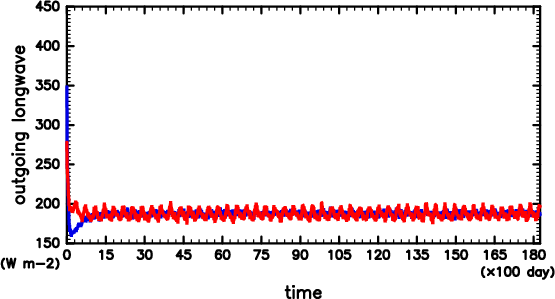
\includegraphics[width=\columnwidth]{S1366/S1366_OLRA-OSRA_horimean_time0.0-18250.0-crop.png}
		\caption{\(S=1366\hmu{W/m^2}\)}\label{S1366_OLRA}
	\end{subfigure}
	\begin{subfigure}{.4\textwidth}
		\centering
		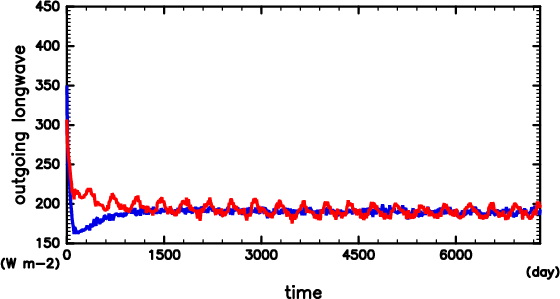
\includegraphics[width=\columnwidth]{S1500/S1500_OLRA-OSRA_horimean_time0.0-7300.0-crop.png}
		\caption{\(S=1500\hmu{W/m^2}\)}\label{S1500_OLRA}
	\end{subfigure}
	\begin{subfigure}{.4\textwidth}
		\centering
		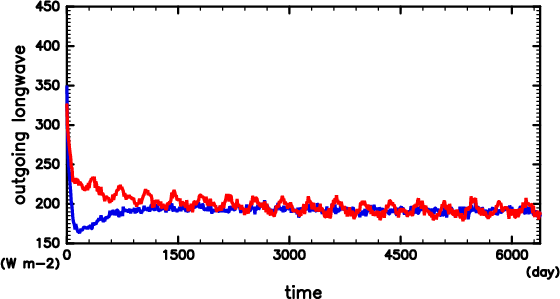
\includegraphics[width=\columnwidth]{S1600/S1600_OLRA-OSRA_horimean_time0.0-7300.0-crop.png}
		\caption{\(S=1600\hmu{W/m^2}\)}\label{S1600_OLRA}
	\end{subfigure}
	\begin{subfigure}{.4\textwidth}
		\centering
		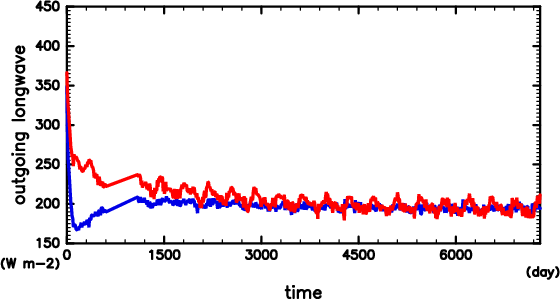
\includegraphics[width=\columnwidth]{S1800/S1800_OLRA-OSRA_horimean_time0.0-7300.0-crop.png}
		\caption{\(S=1800\hmu{W/m^2}\)}\label{S1800_OLRA}
	\end{subfigure}
	\begin{subfigure}{.4\textwidth}
		\centering
		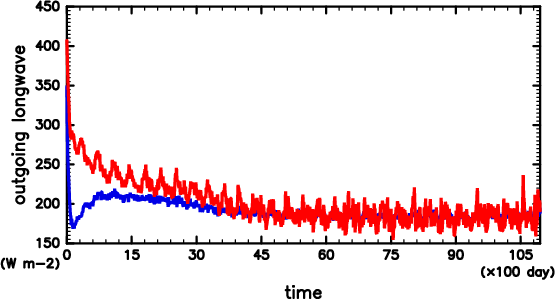
\includegraphics[width=\columnwidth]{S2000/S2000_OLRA-OSRA_horimean_time0.0-10950.0-crop.png}
		\caption{\(S=2000\hmu{W/m^2}\)}\label{S2000_OLRA}
	\end{subfigure}
	\caption{各実験での全球平均した OLR(赤線)と OSR(青線)の時系列変化}\label{OLR-OSR}
\end{figure}

\begin{figure}[t]
	\centering
	\begin{minipage}{.45\textwidth}
		\centering
		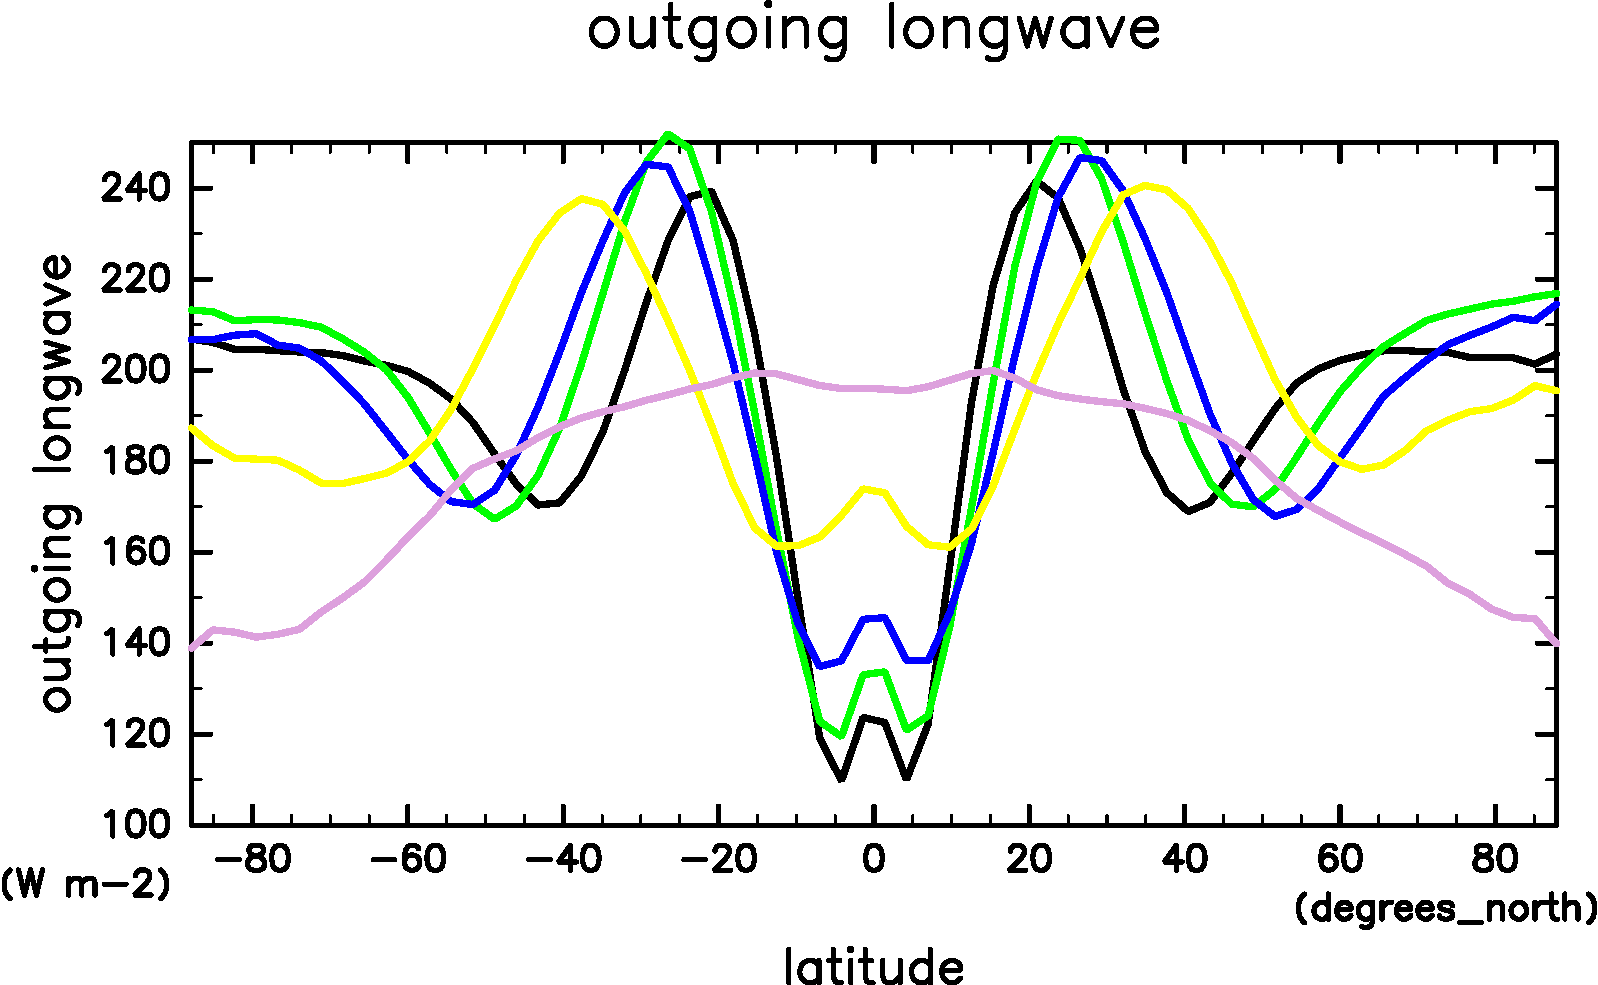
\includegraphics[width=\textwidth]{OLR-overplot-crop-rotate.pdf}
		\caption[各実験での OLR の東西平均]{
			各実験での OLR の東西平均。それぞれ、黒線: S1366;
			緑線: S1500; 青線: S1600; 黄線: S1800; 桃線: S2000 の結果である。
		}\label{OLR東西平均}
	\end{minipage}
	\hfill
	\begin{minipage}{.45\textwidth}
		\centering
		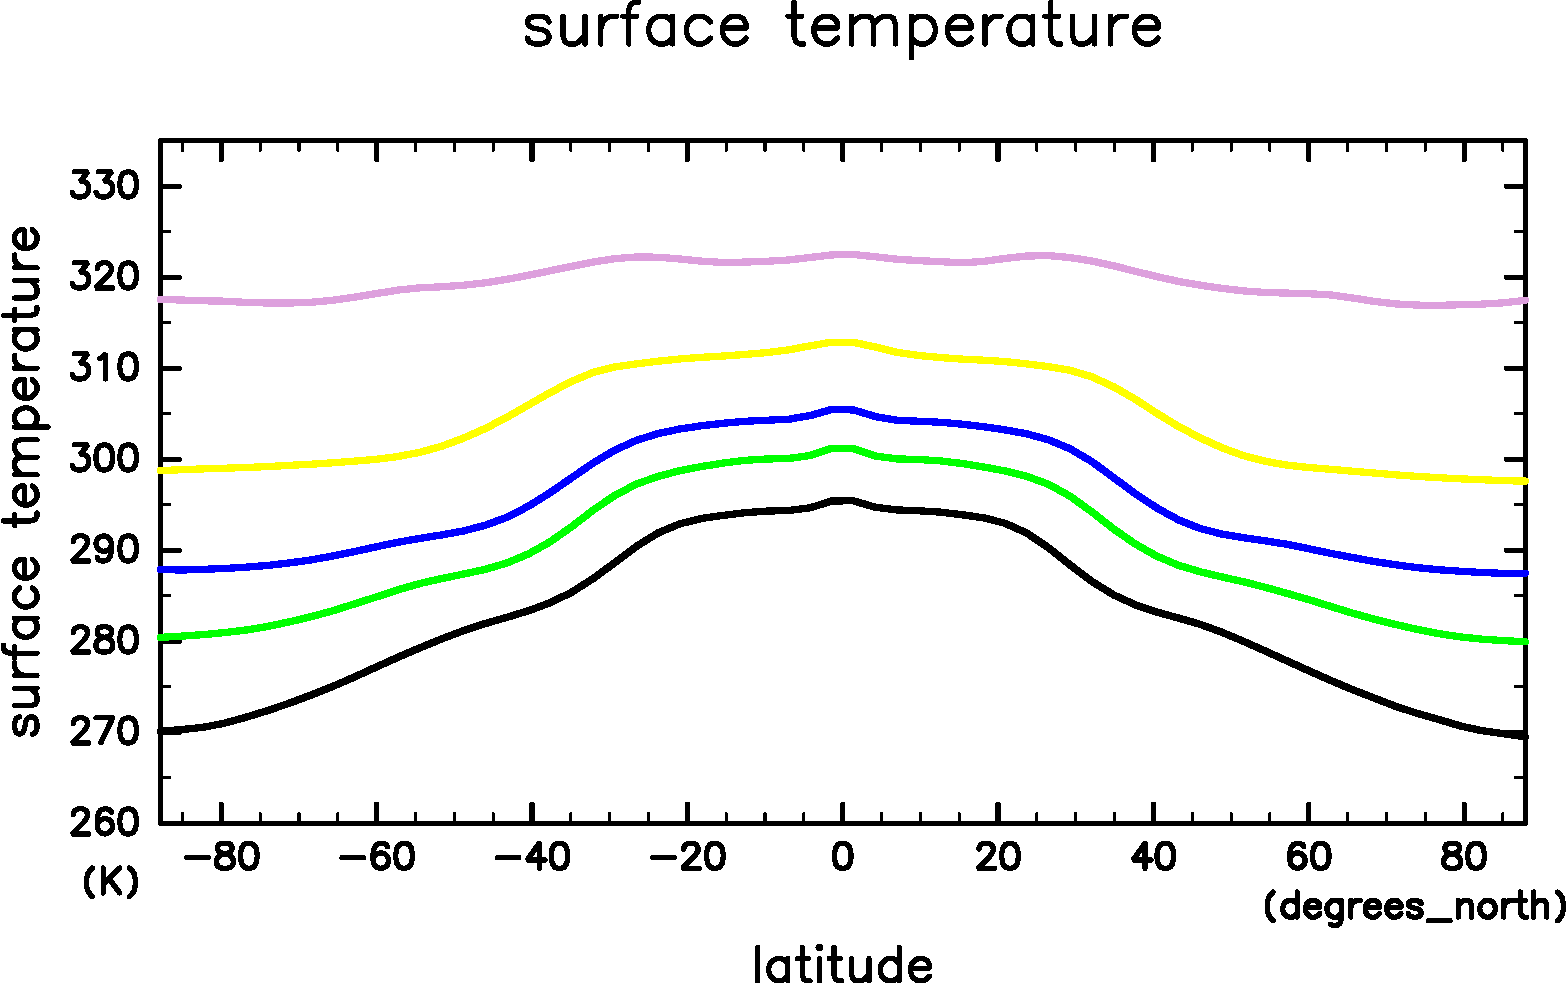
\includegraphics[width=\textwidth]{SurfTemp-overplot-crop-rotate.pdf}
		\caption[各実験での地表面温度の東西平均]{
			各実験での地表面温度の東西平均。それぞれ、黒線: S1366;
			緑線: S1500; 青線: S1600; 黄線: S1800; 桃線: S2000 の結果である。
		}\label{地表面温度}
	\end{minipage}
\end{figure}

次に、各実験で得られた大気構造がどのようになっているか詳細に見てゆこう。
各実験で得られた子午面構造を図 \ref{S1366} から \ref{S2000} に示す。
いずれの実験でも、東西風の子午面分布(図 \ref{S1366東西風} から \ref{S2000東西風})
を確認すると、ジェットが発生しているのがわかる。
しかし、S1800 と S2000 ではジェットが大気上端に
くっついており、モデルの高度が足りていない可能性がある。

\begin{figure}[t]
	\centering
	\begin{subfigure}{.4\textwidth}
		\centering
		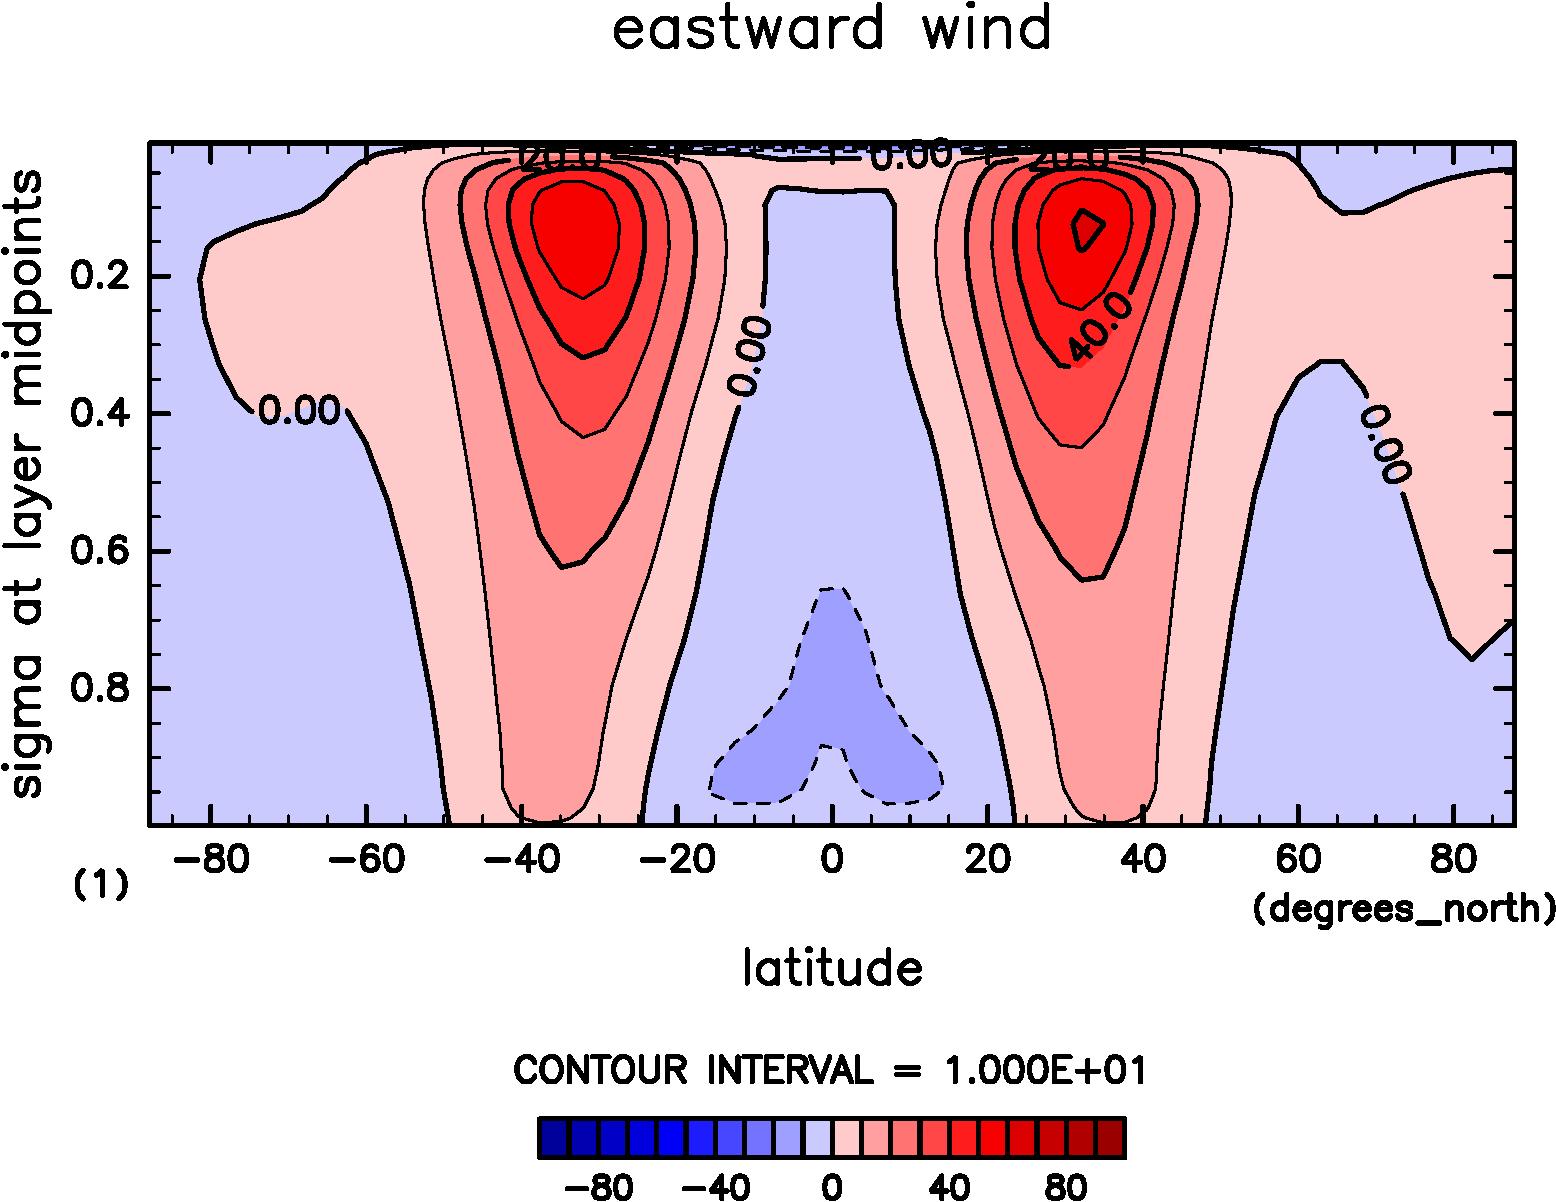
\includegraphics[width=\columnwidth]{S1366/U,time=14600:14965-crop-rotate.pdf}
		\caption{東西風}\label{S1366東西風}
	\end{subfigure}
	\begin{subfigure}{.4\textwidth}
		\centering
		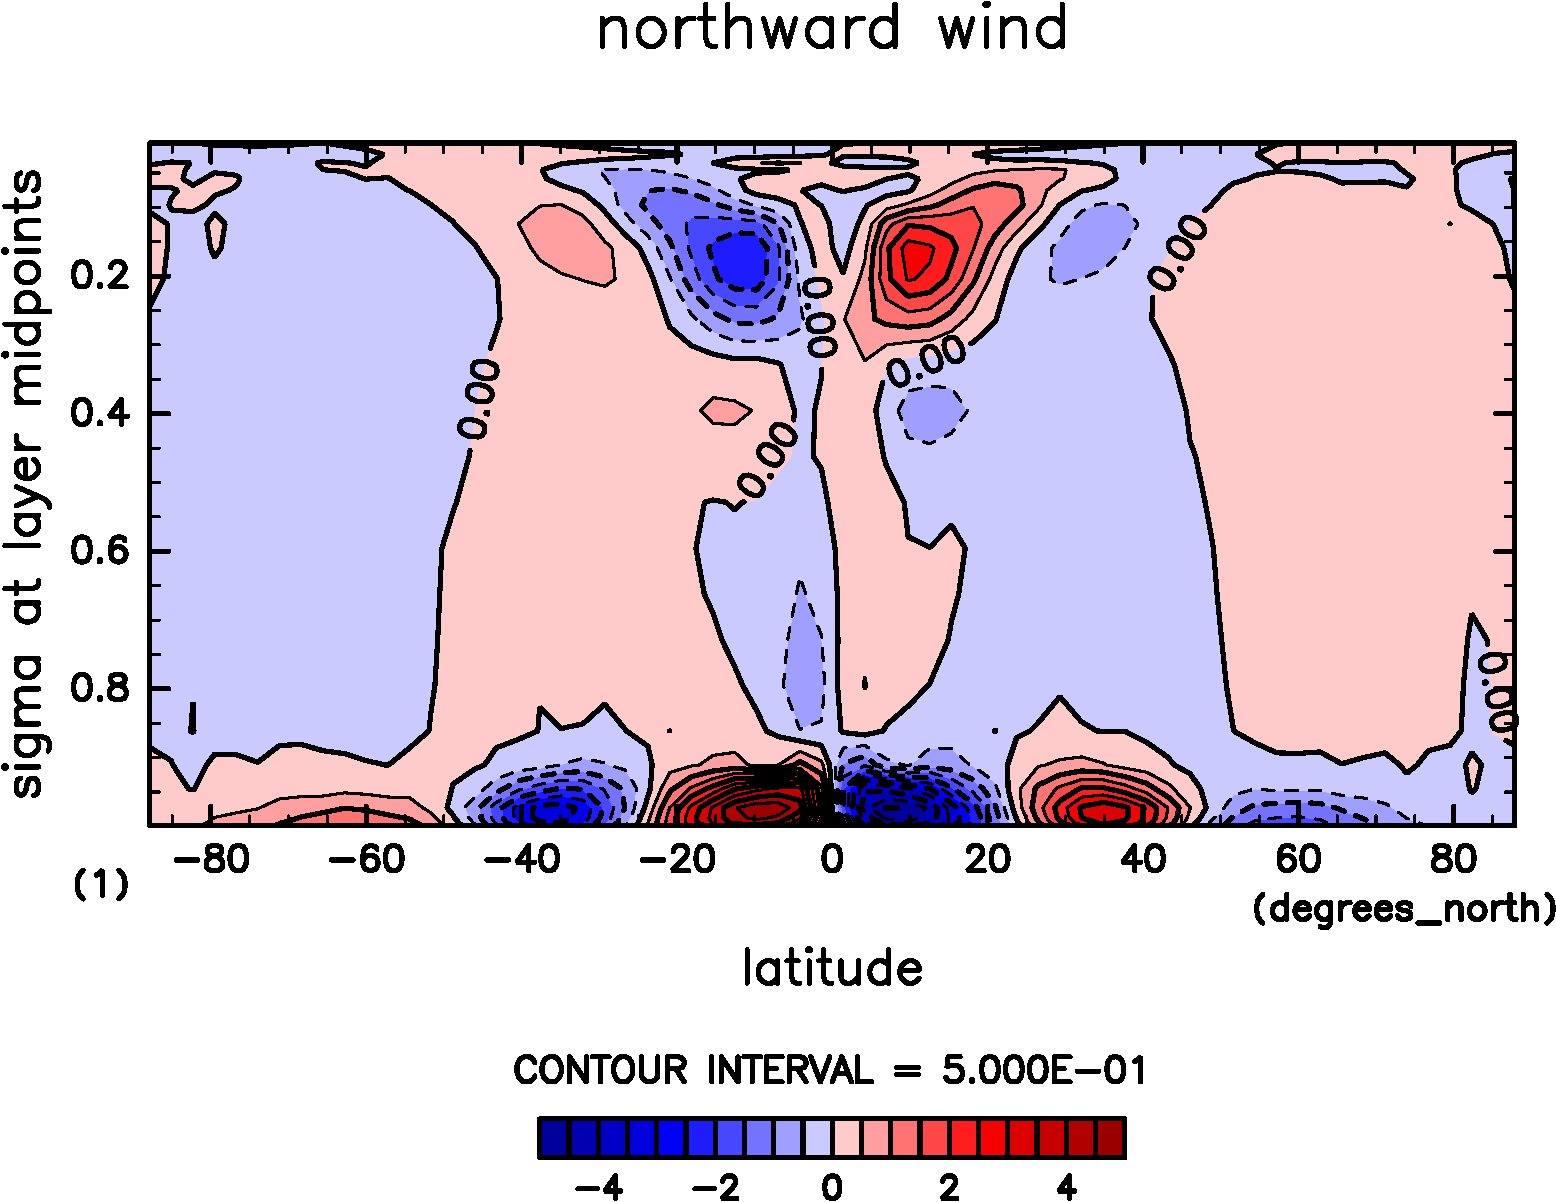
\includegraphics[width=\columnwidth]{S1366/V,time=14600:14965-crop-rotate.pdf}
		\caption{南北風}\label{S1366南北風}
	\end{subfigure}
	\begin{subfigure}{.4\textwidth}
		\centering
		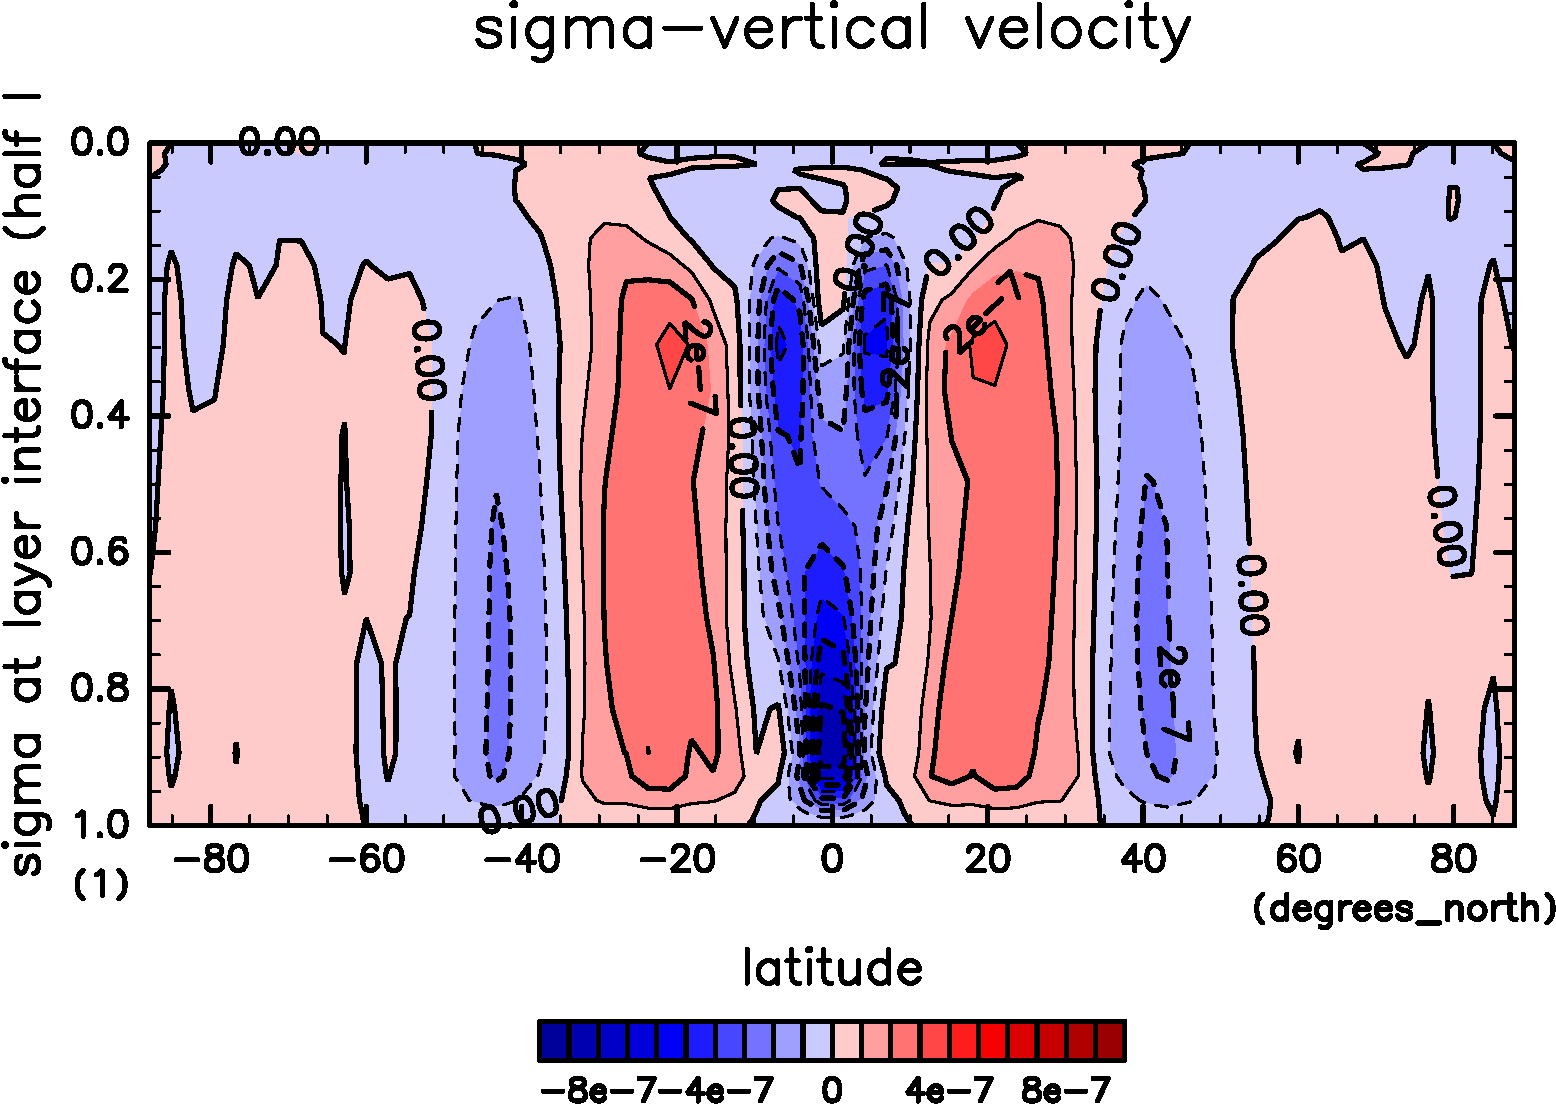
\includegraphics[width=\columnwidth]{S1366/SigDot,time=14600:14965-crop-rotate.pdf}
		\caption{鉛直風}\label{S1366鉛直風}
	\end{subfigure}
	\begin{subfigure}{.4\textwidth}
		\centering
		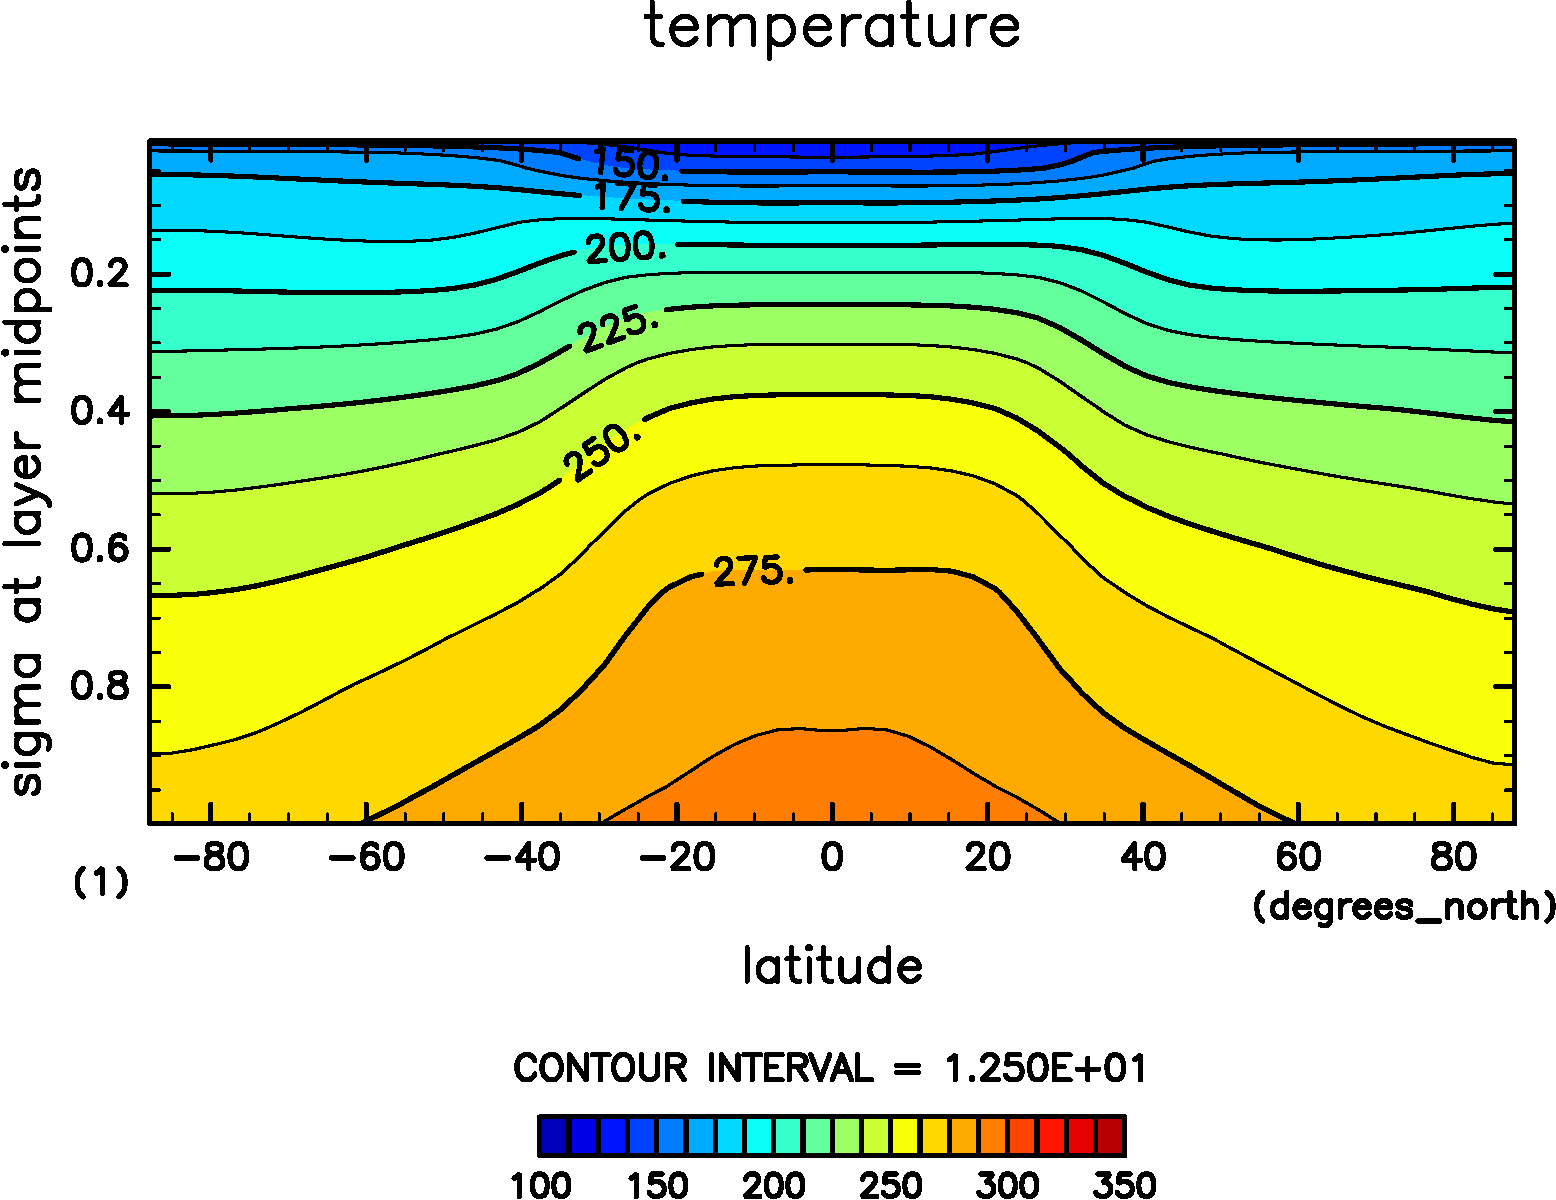
\includegraphics[width=\columnwidth]{S1366/Temp,time=14600:14965-crop-rotate.pdf}
		\caption{気温分布}\label{S1366気温分布}
	\end{subfigure}
	\begin{subfigure}{.4\textwidth}
		\centering
		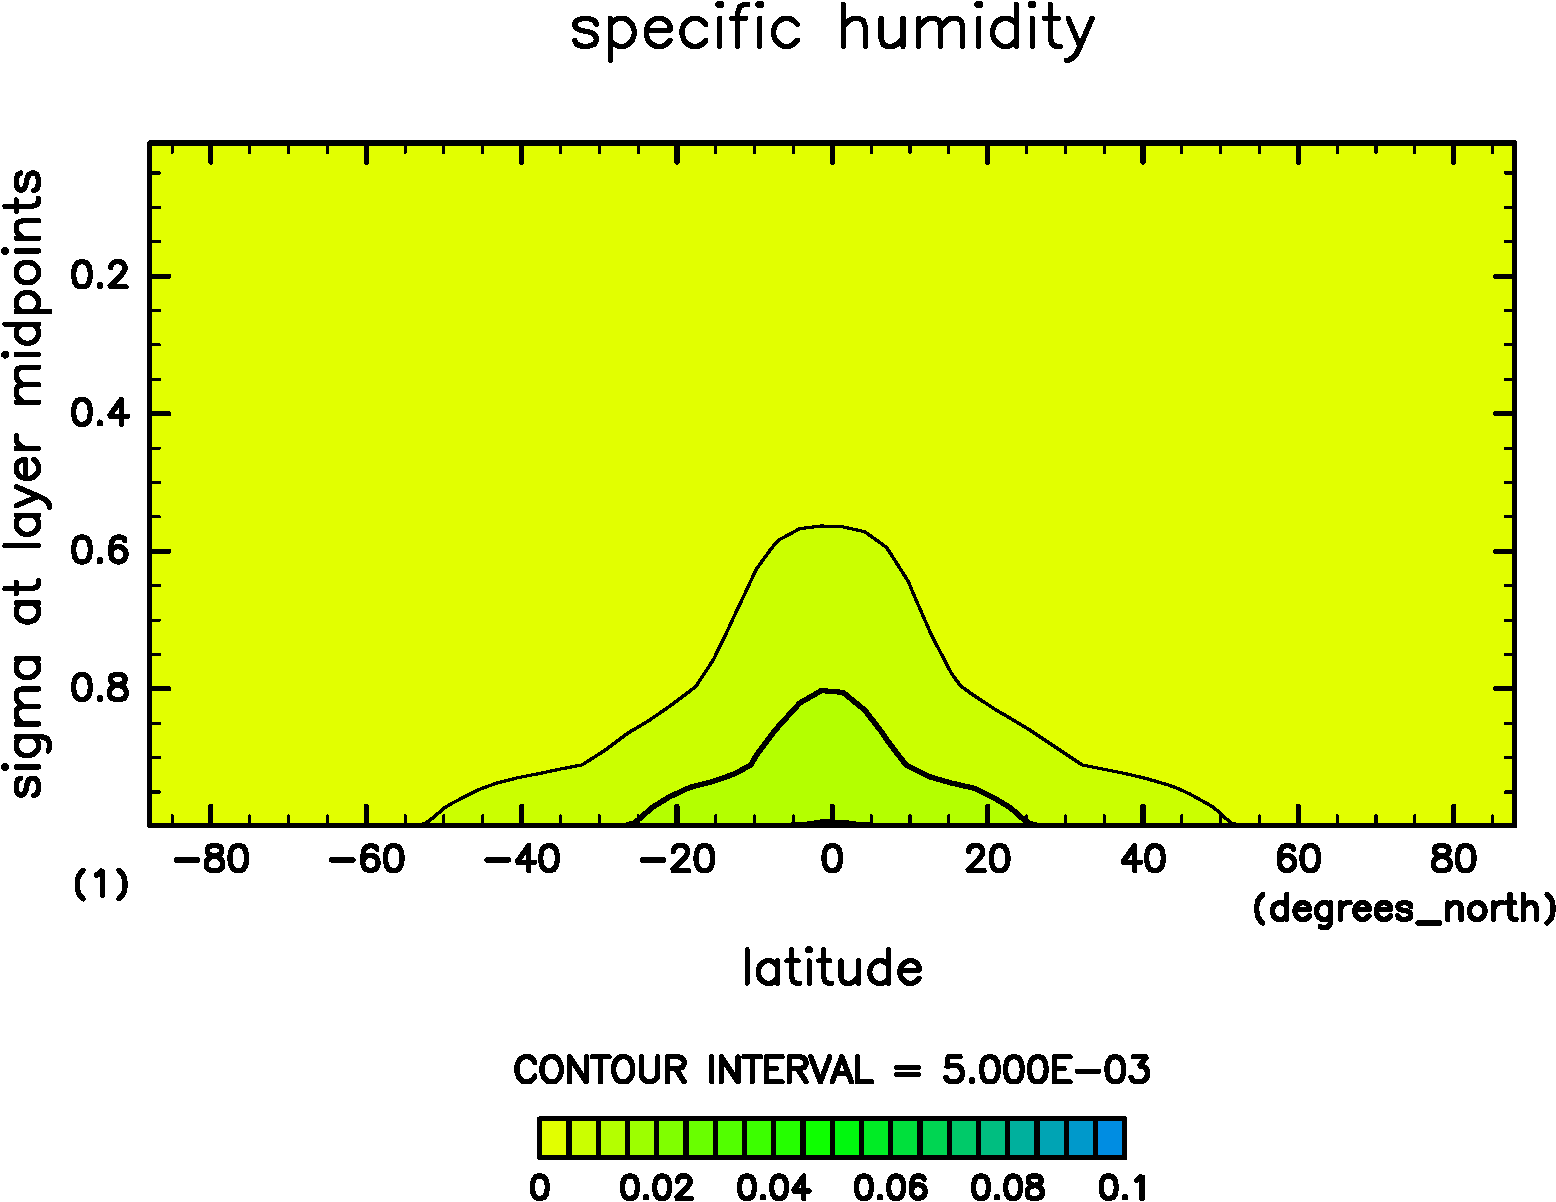
\includegraphics[width=\columnwidth]{S1366/QH2OVap,time=14600:14965-crop-rotate.pdf}
		\caption{比湿}\label{S1366比湿}
	\end{subfigure}
	\begin{subfigure}{.4\textwidth}
		\centering
		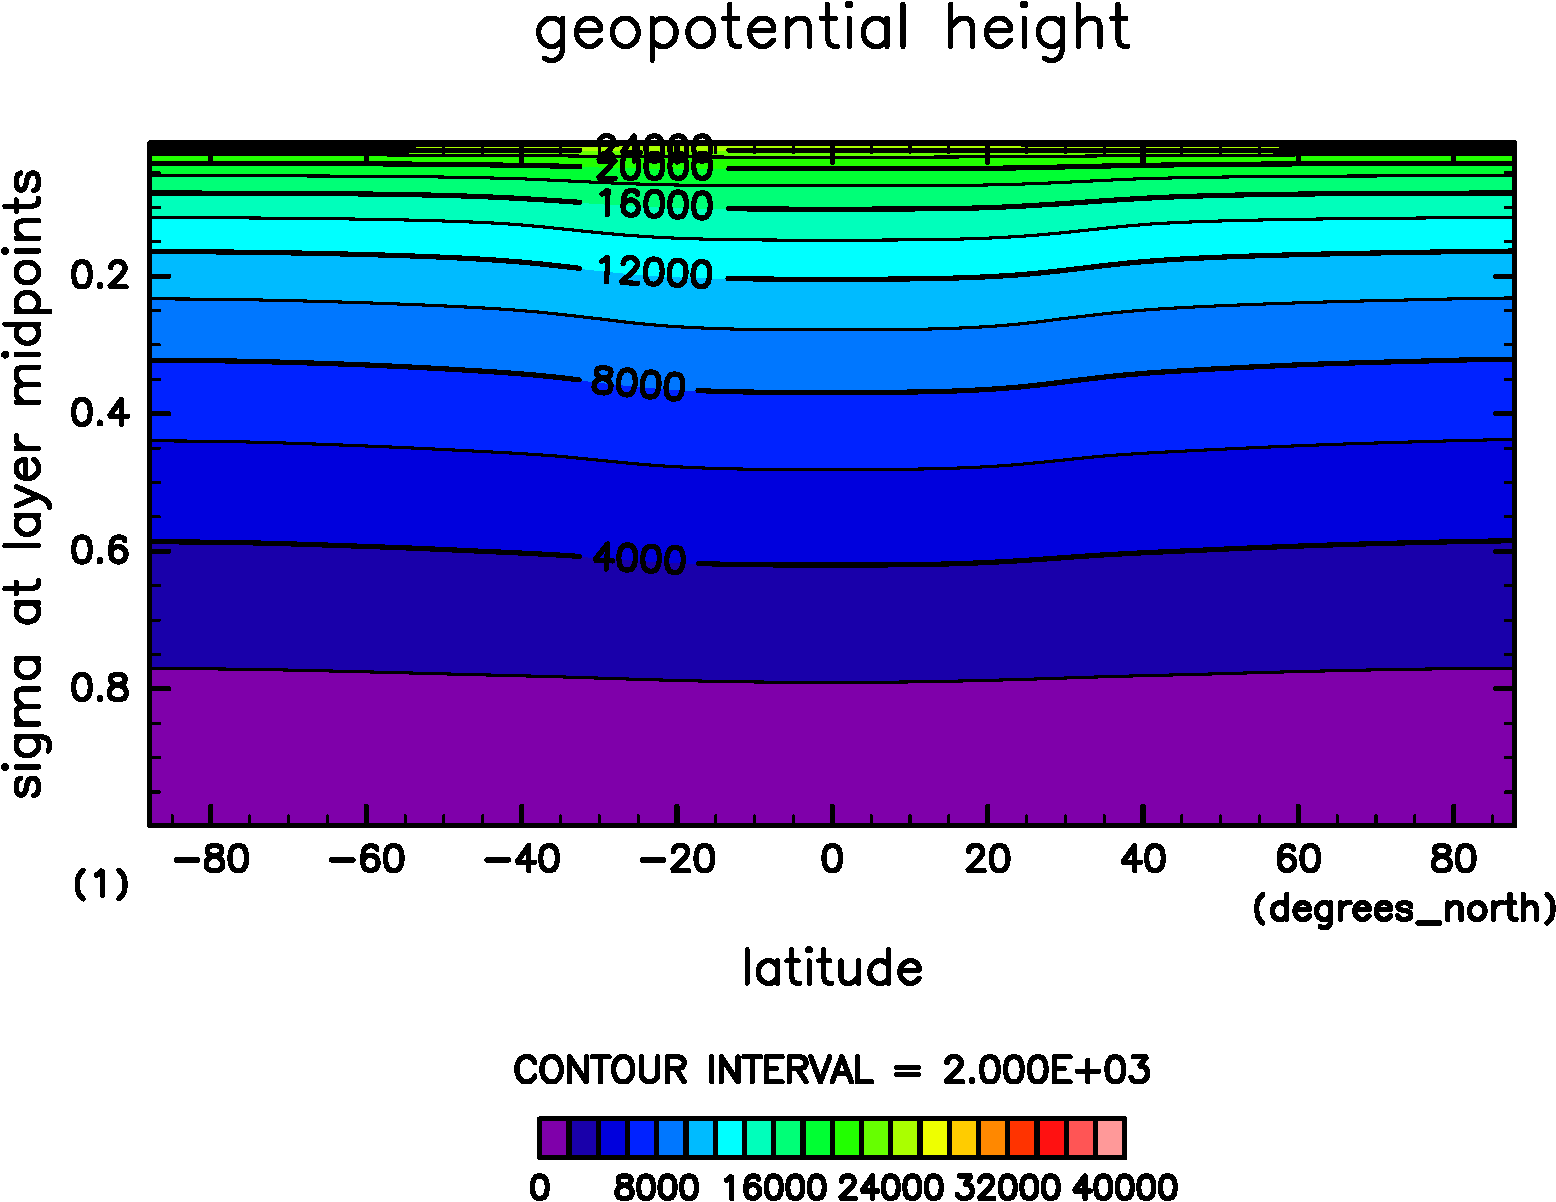
\includegraphics[width=\columnwidth]{S1366/Height,time=14600:14965-crop-rotate.pdf}
		\caption{ジオポテンシャル高度}\label{S1366ジオポテンシャル高度}
	\end{subfigure}
	\caption{
		\(S=1366\hmu{W/m^2}\) の結果。11 年目の年平均値。
	}\label{S1366}
\end{figure}

\begin{figure}[t]
	\centering
	\begin{subfigure}{.4\textwidth}
		\centering
		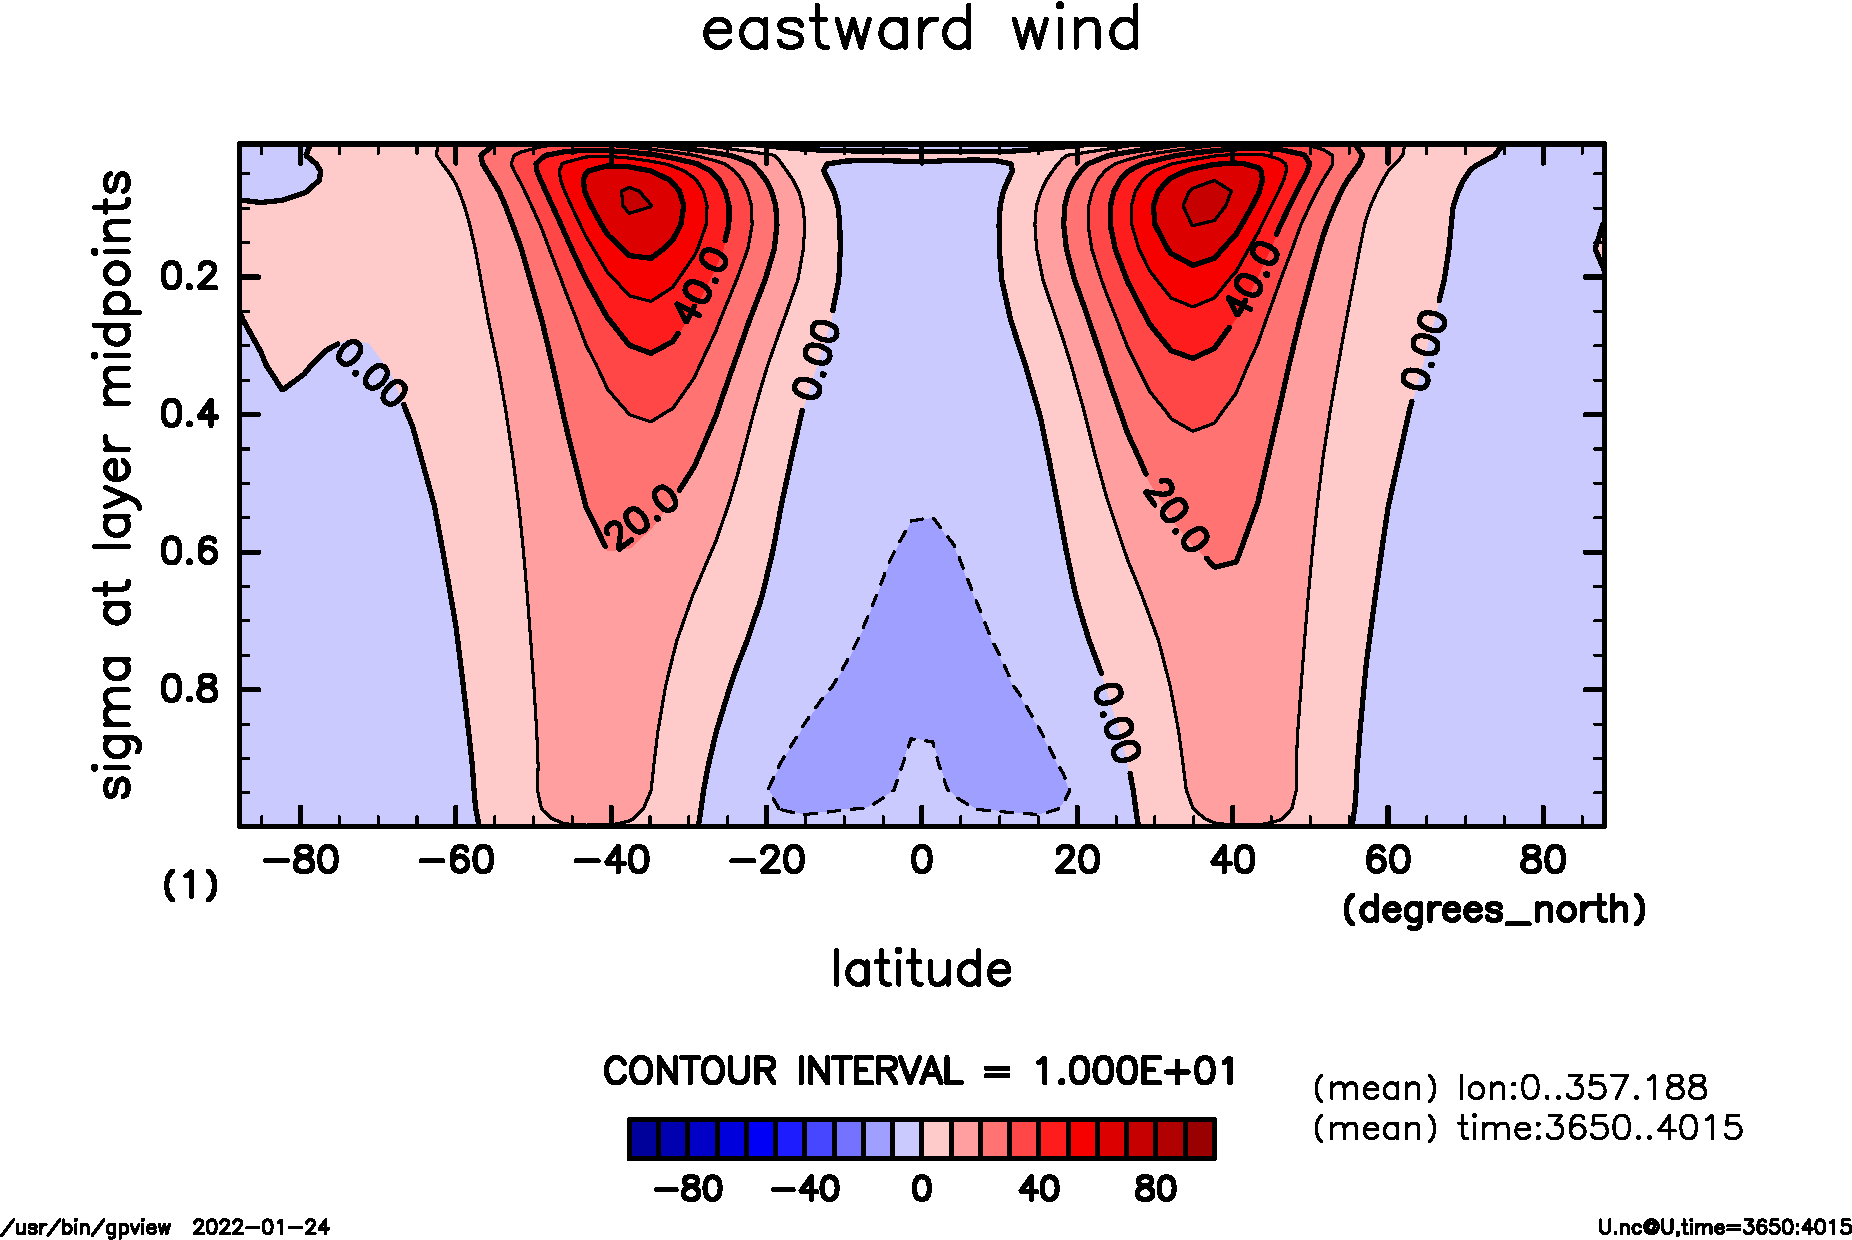
\includegraphics[width=\columnwidth]{S1500/U,time=3650:4015-crop-rotate.pdf}
		\caption{東西風}\label{S1500東西風}
	\end{subfigure}
	\begin{subfigure}{.4\textwidth}
		\centering
		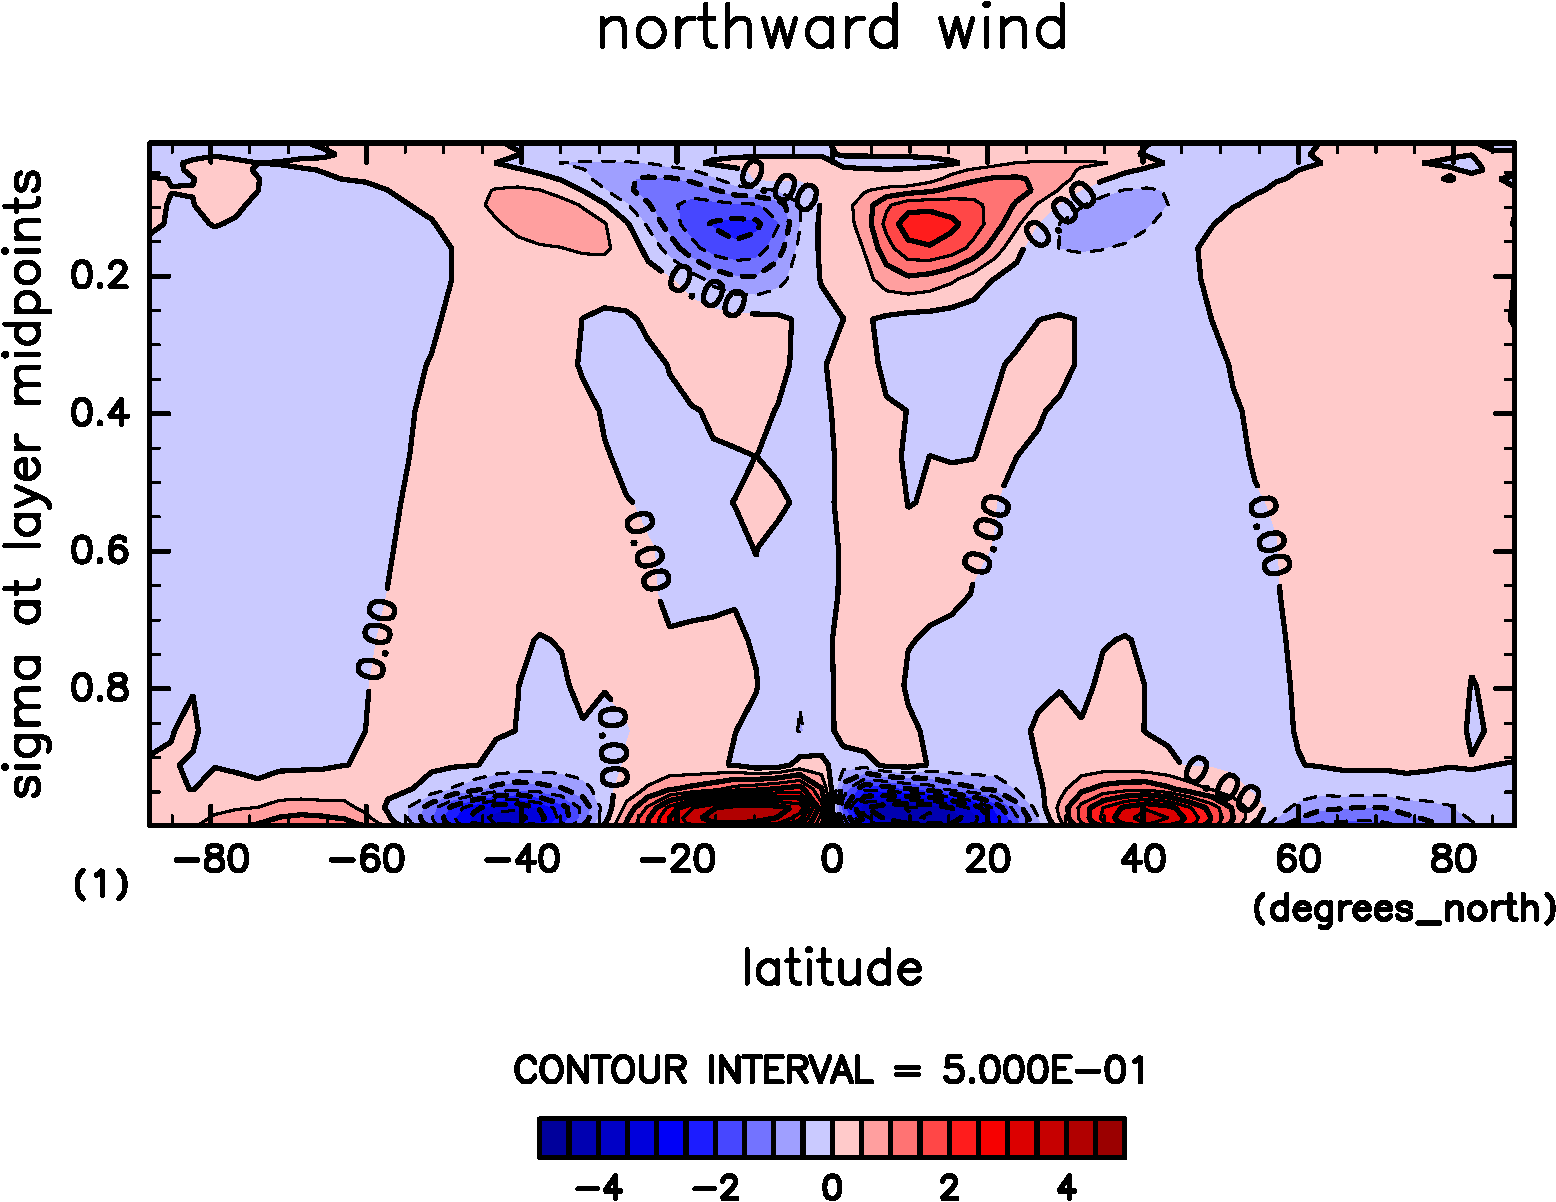
\includegraphics[width=\columnwidth]{S1500/V,time=3650:4015-crop-rotate.pdf}
		\caption{南北風}\label{S1500南北風}
	\end{subfigure}
	\begin{subfigure}{.4\textwidth}
		\centering
		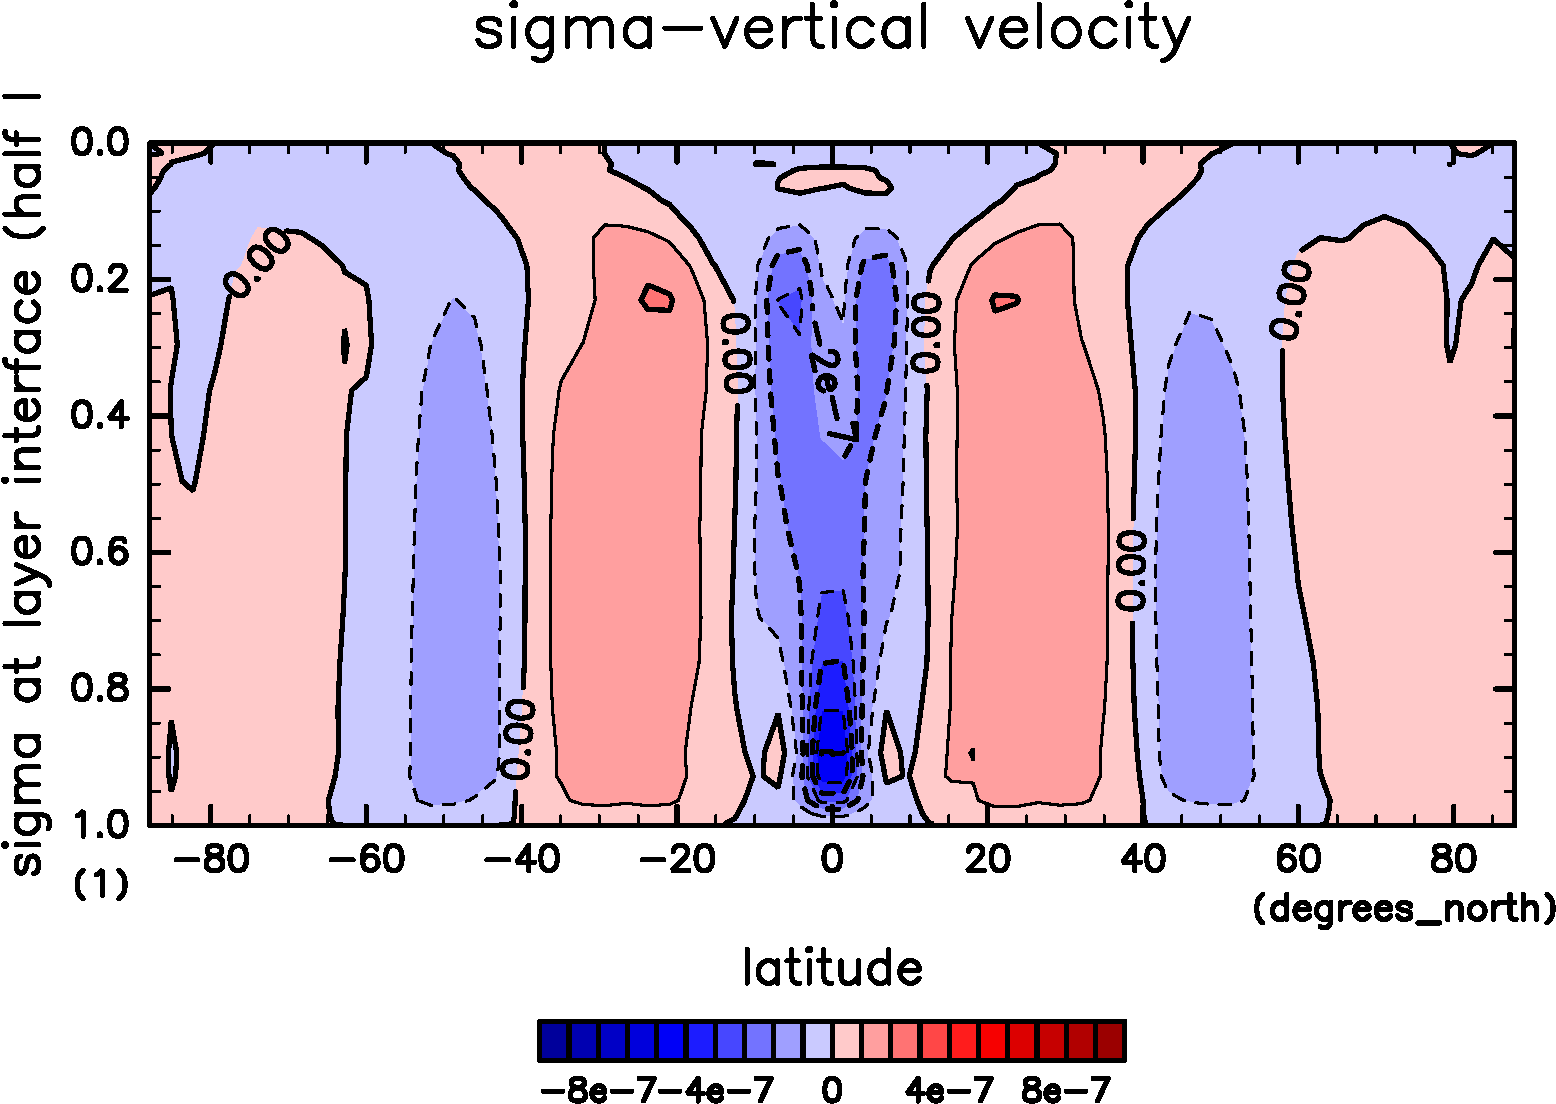
\includegraphics[width=\columnwidth]{S1500/SigDot,time=3650:4015-crop-rotate.pdf}
		\caption{鉛直風}\label{S1500鉛直風}
	\end{subfigure}
	\begin{subfigure}{.4\textwidth}
		\centering
		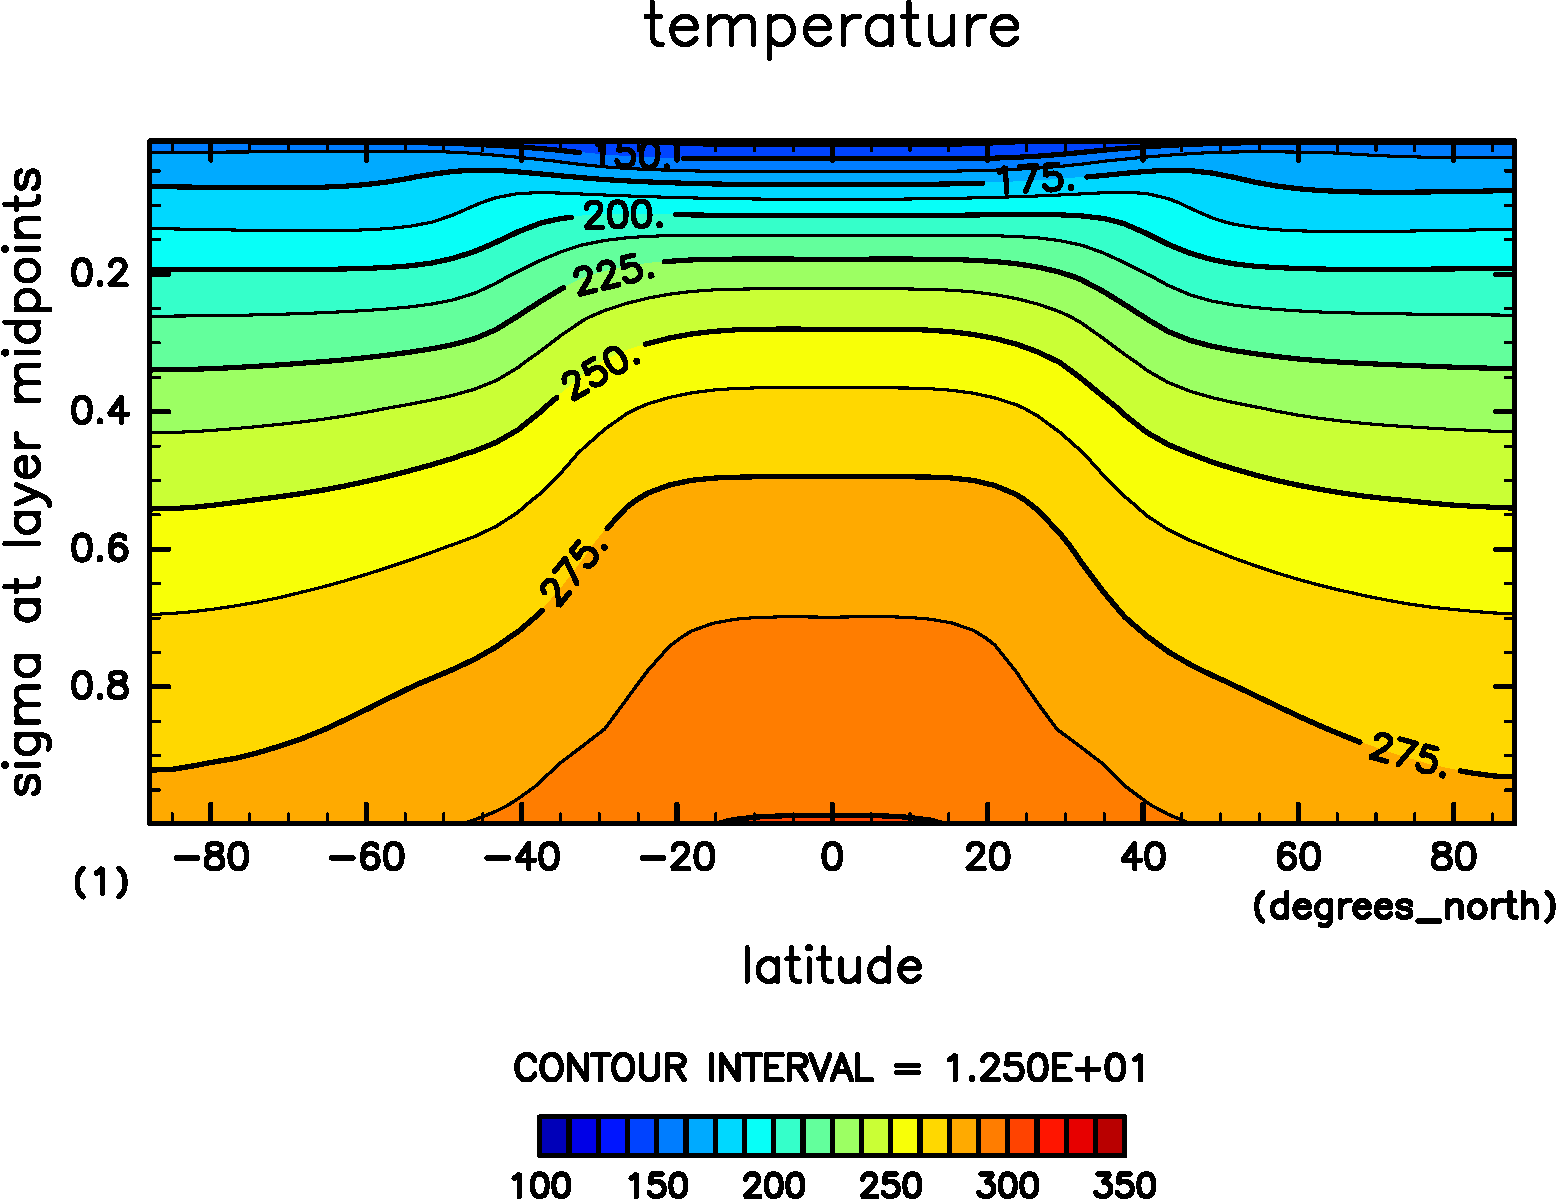
\includegraphics[width=\columnwidth]{S1500/Temp,time=3650:4015-crop-rotate.pdf}
		\caption{気温分布}\label{S1500気温分布}
	\end{subfigure}
	\begin{subfigure}{.4\textwidth}
		\centering
		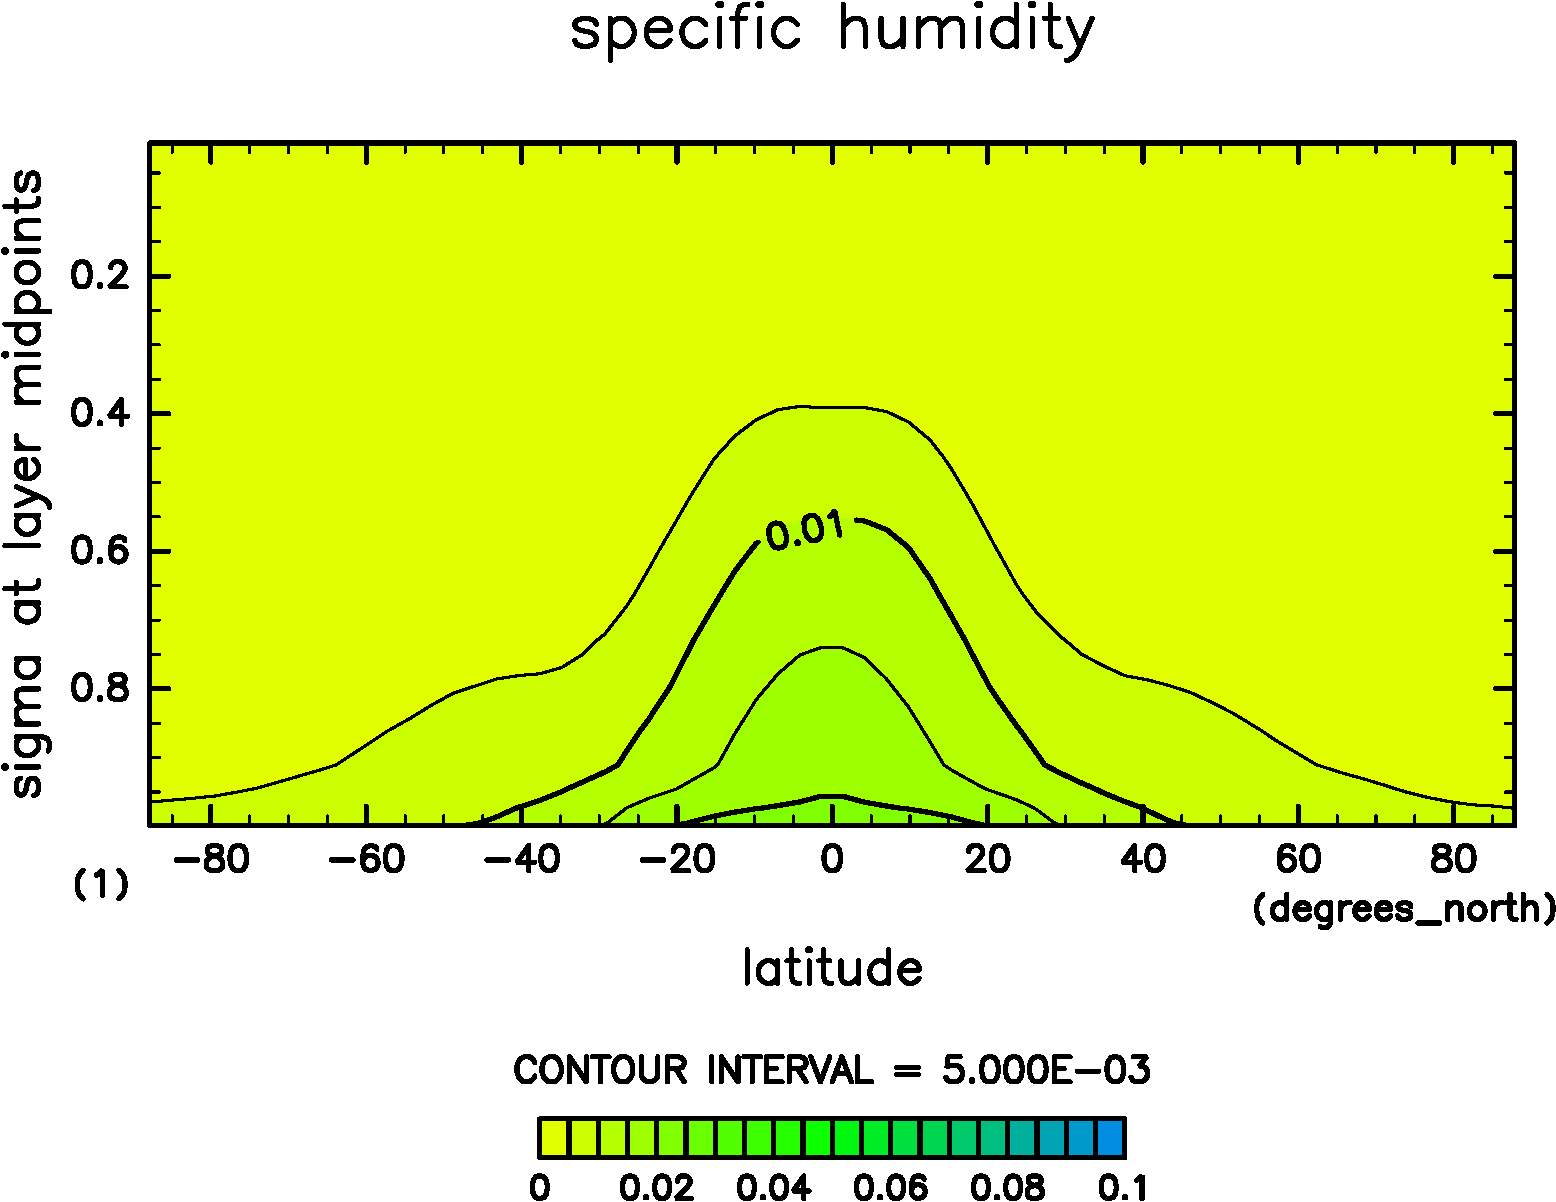
\includegraphics[width=\columnwidth]{S1500/QH2OVap,time=3650:4015-crop-rotate.pdf}
		\caption{比湿}\label{S1500比湿}
	\end{subfigure}
	\begin{subfigure}{.4\textwidth}
		\centering
		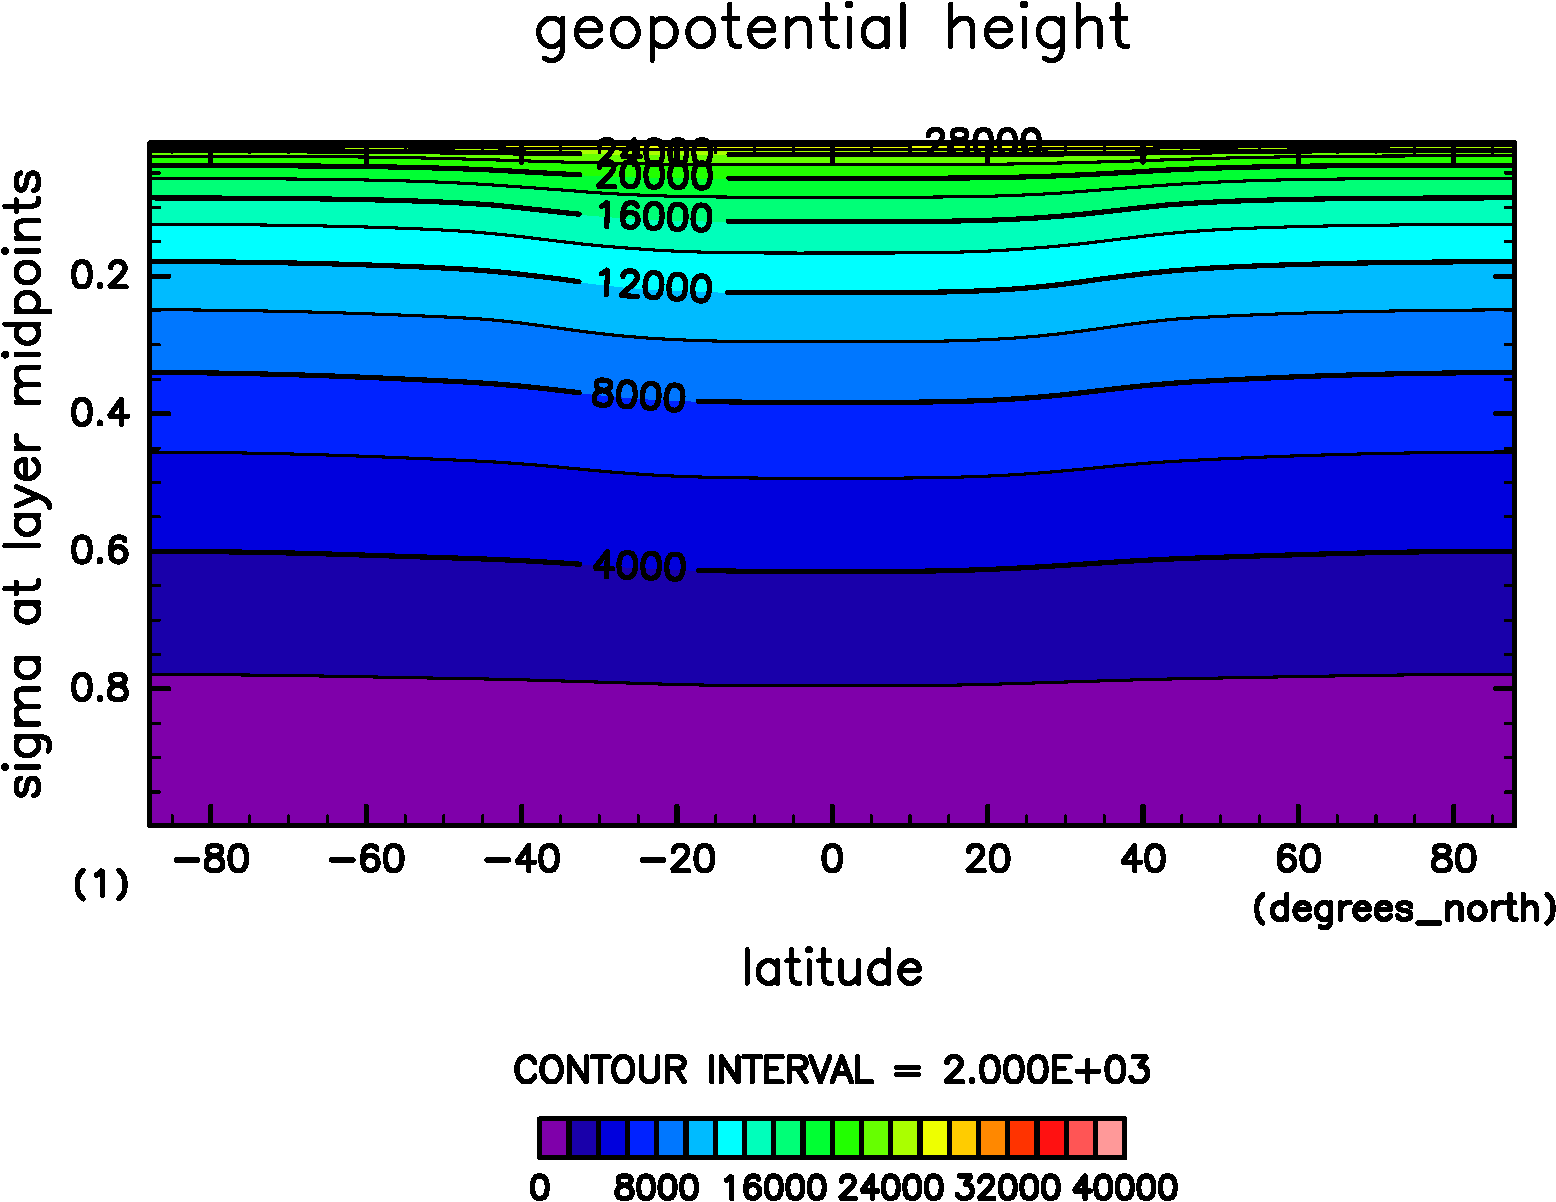
\includegraphics[width=\columnwidth]{S1500/Height,time=3650:4015-crop-rotate.pdf}
		\caption{ジオポテンシャル高度}\label{S1500ジオポテンシャル高度}
	\end{subfigure}
	\caption{
		\(S=1500\hmu{W/m^2}\) の結果。11 年目の年平均値。
	}\label{S1500}
\end{figure}

\begin{figure}[t]
	\centering
	\begin{subfigure}{.4\textwidth}
		\centering
		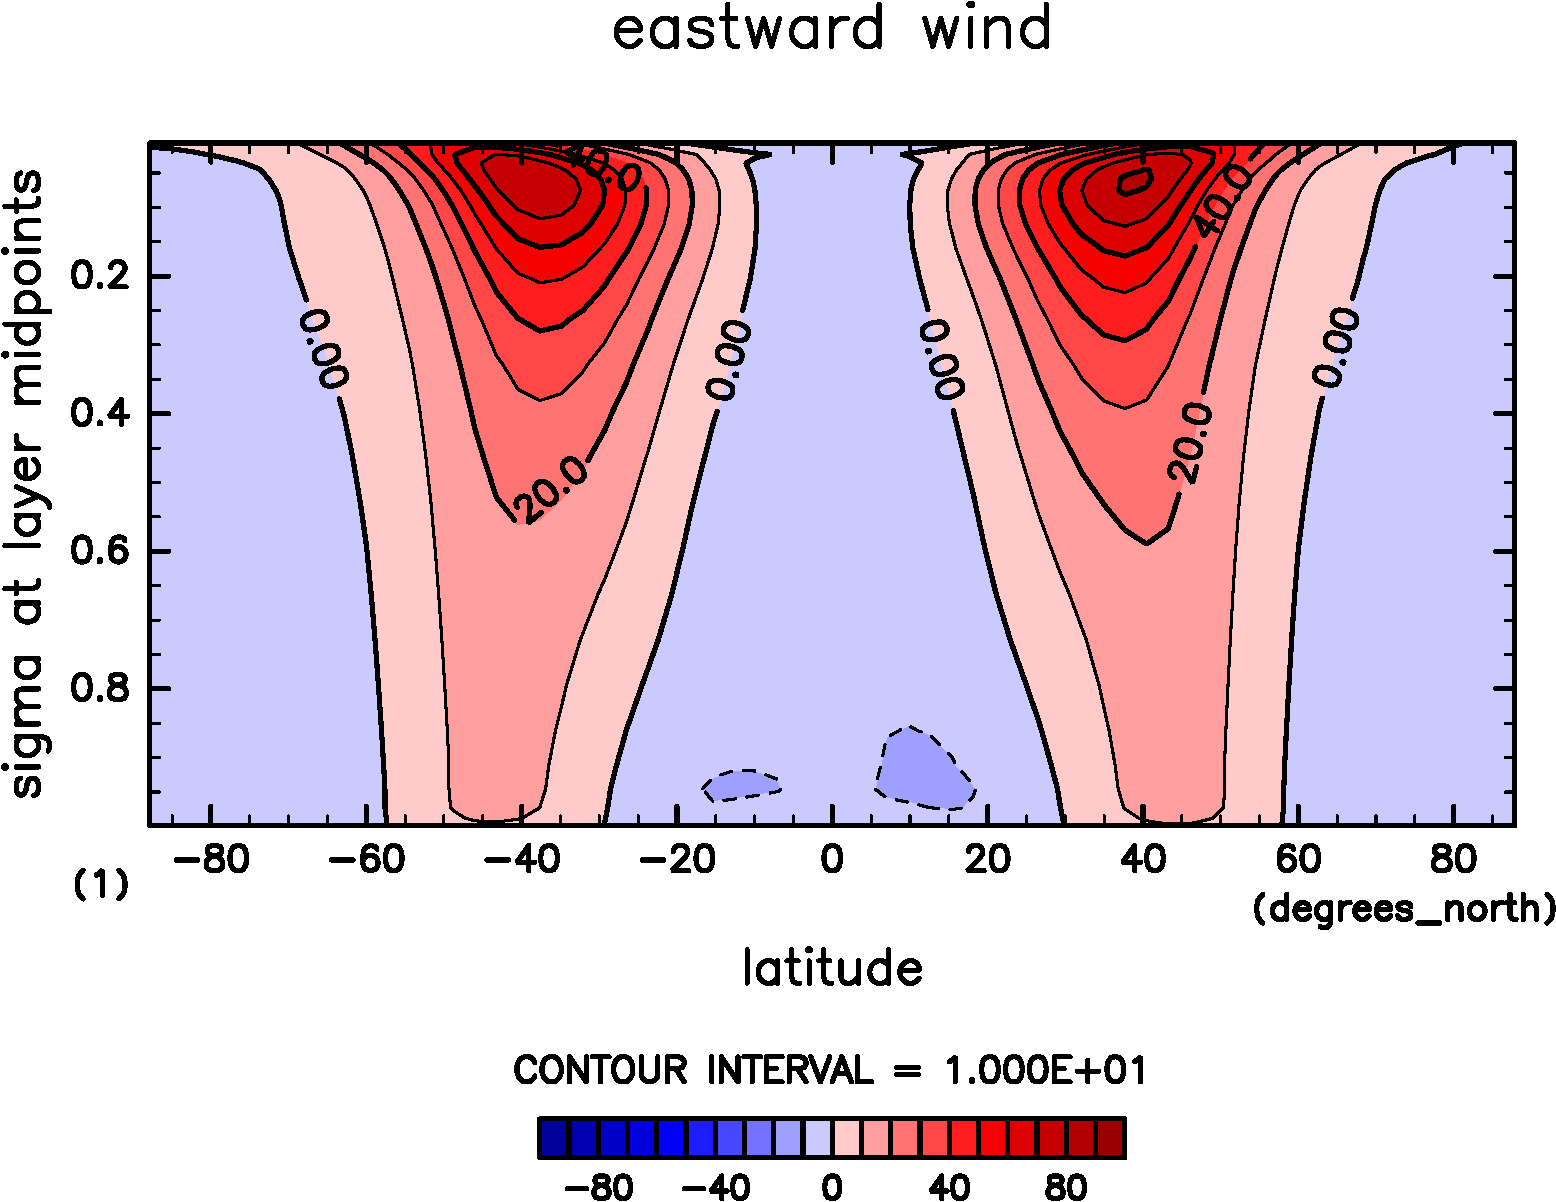
\includegraphics[width=\columnwidth]{S1600/U,time=3650:4015-crop-rotate.pdf}
		\caption{東西風}\label{S1600東西風}
	\end{subfigure}
	\begin{subfigure}{.4\textwidth}
		\centering
		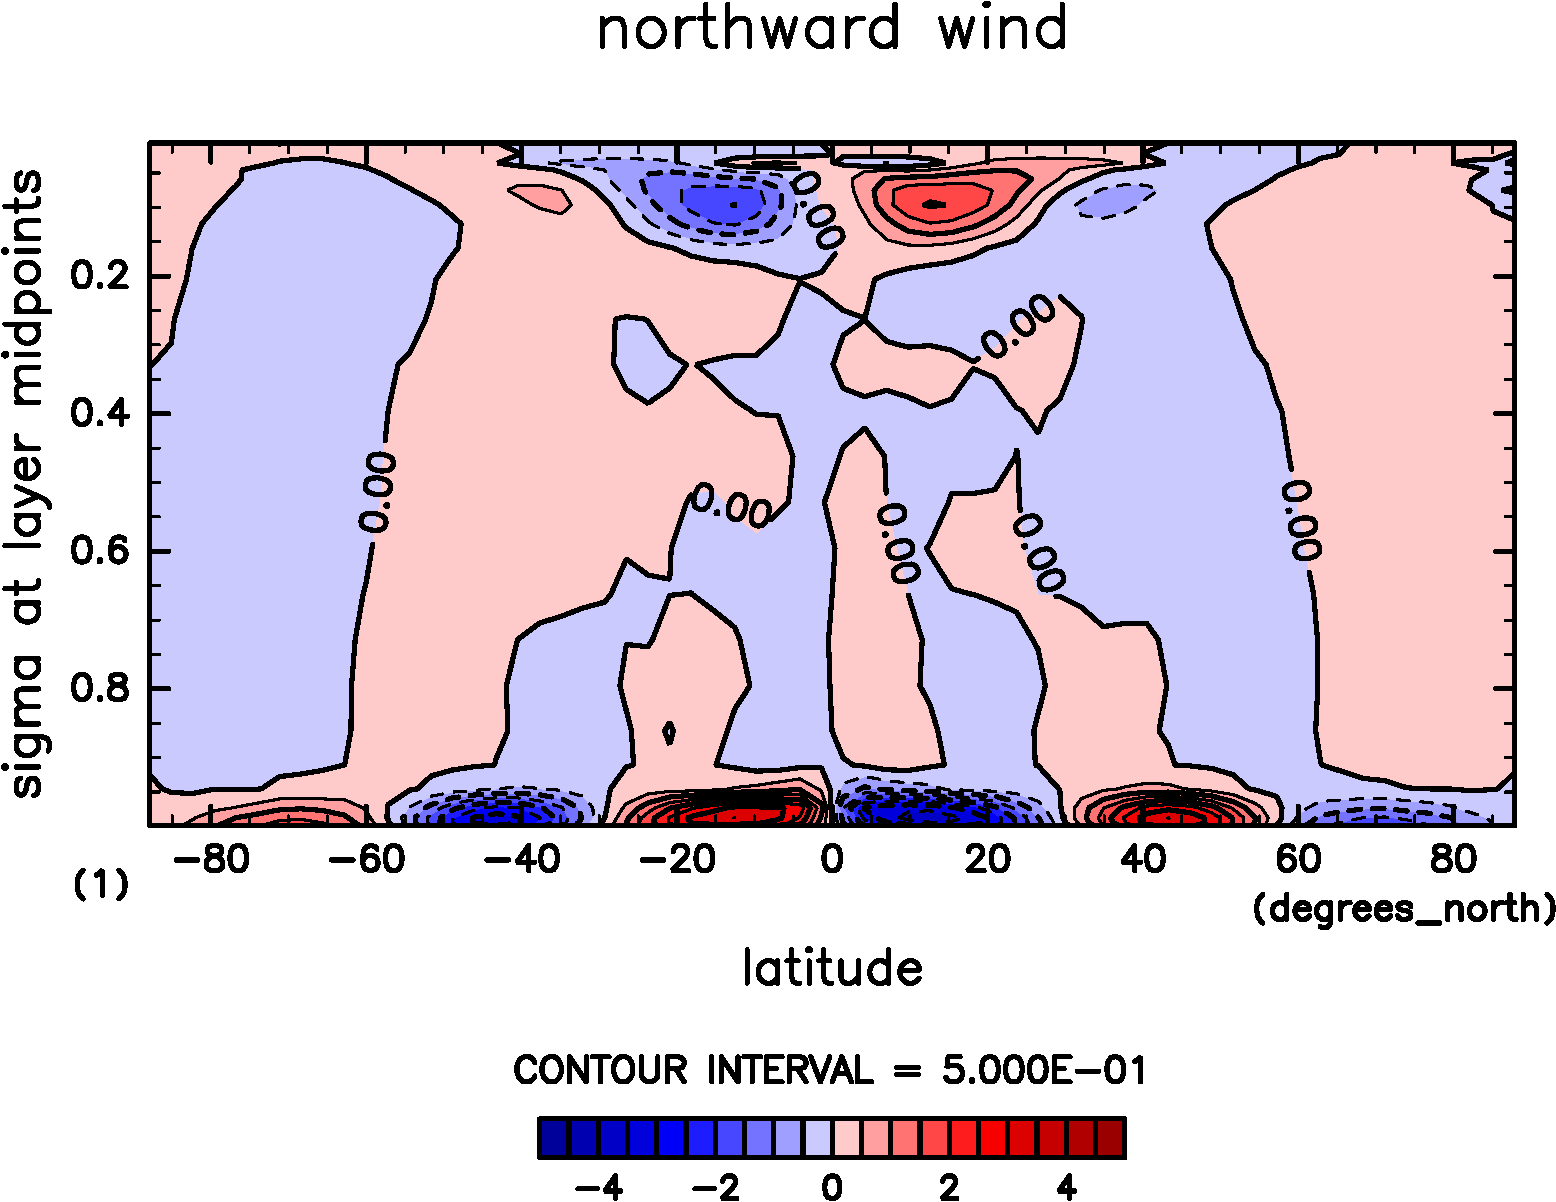
\includegraphics[width=\columnwidth]{S1600/V,time=3650:4015-crop-rotate.pdf}
		\caption{南北風}\label{S1600南北風}
	\end{subfigure}
	\begin{subfigure}{.4\textwidth}
		\centering
		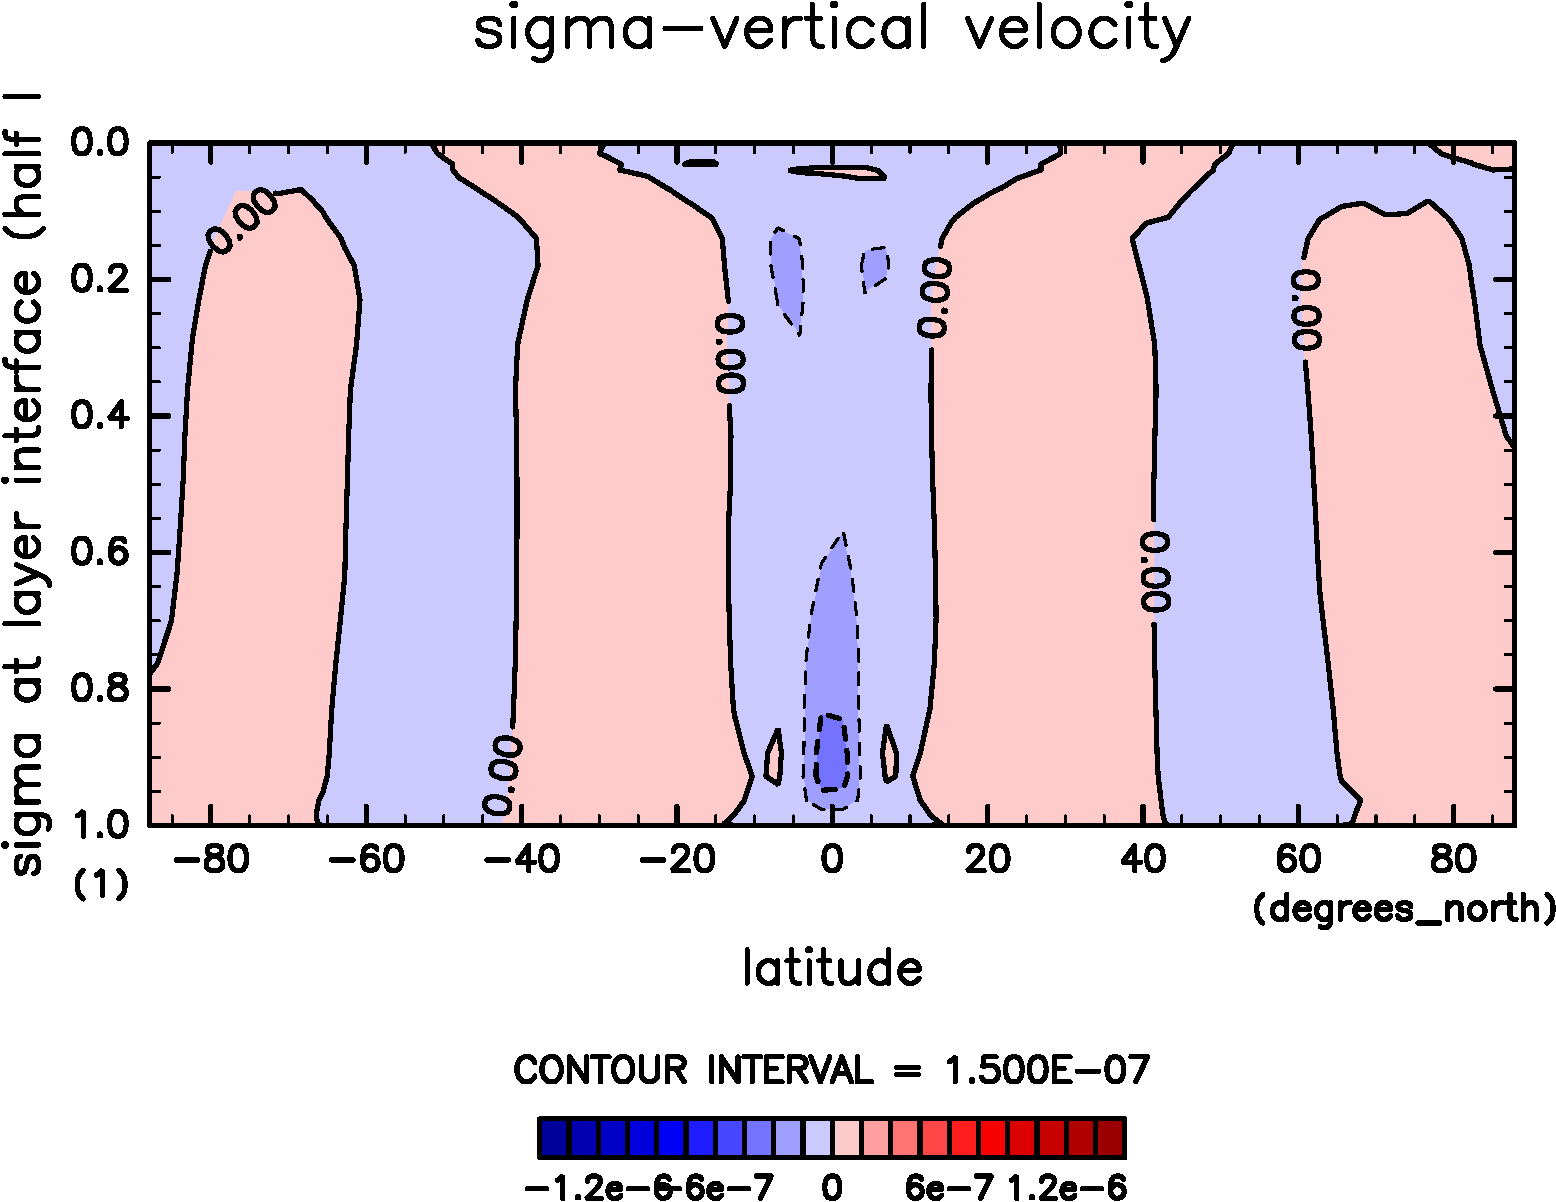
\includegraphics[width=\columnwidth]{S1600/SigDot,time=3650:4015-crop-rotate.pdf}
		\caption{鉛直風}\label{S1600鉛直風}
	\end{subfigure}
	\begin{subfigure}{.4\textwidth}
		\centering
		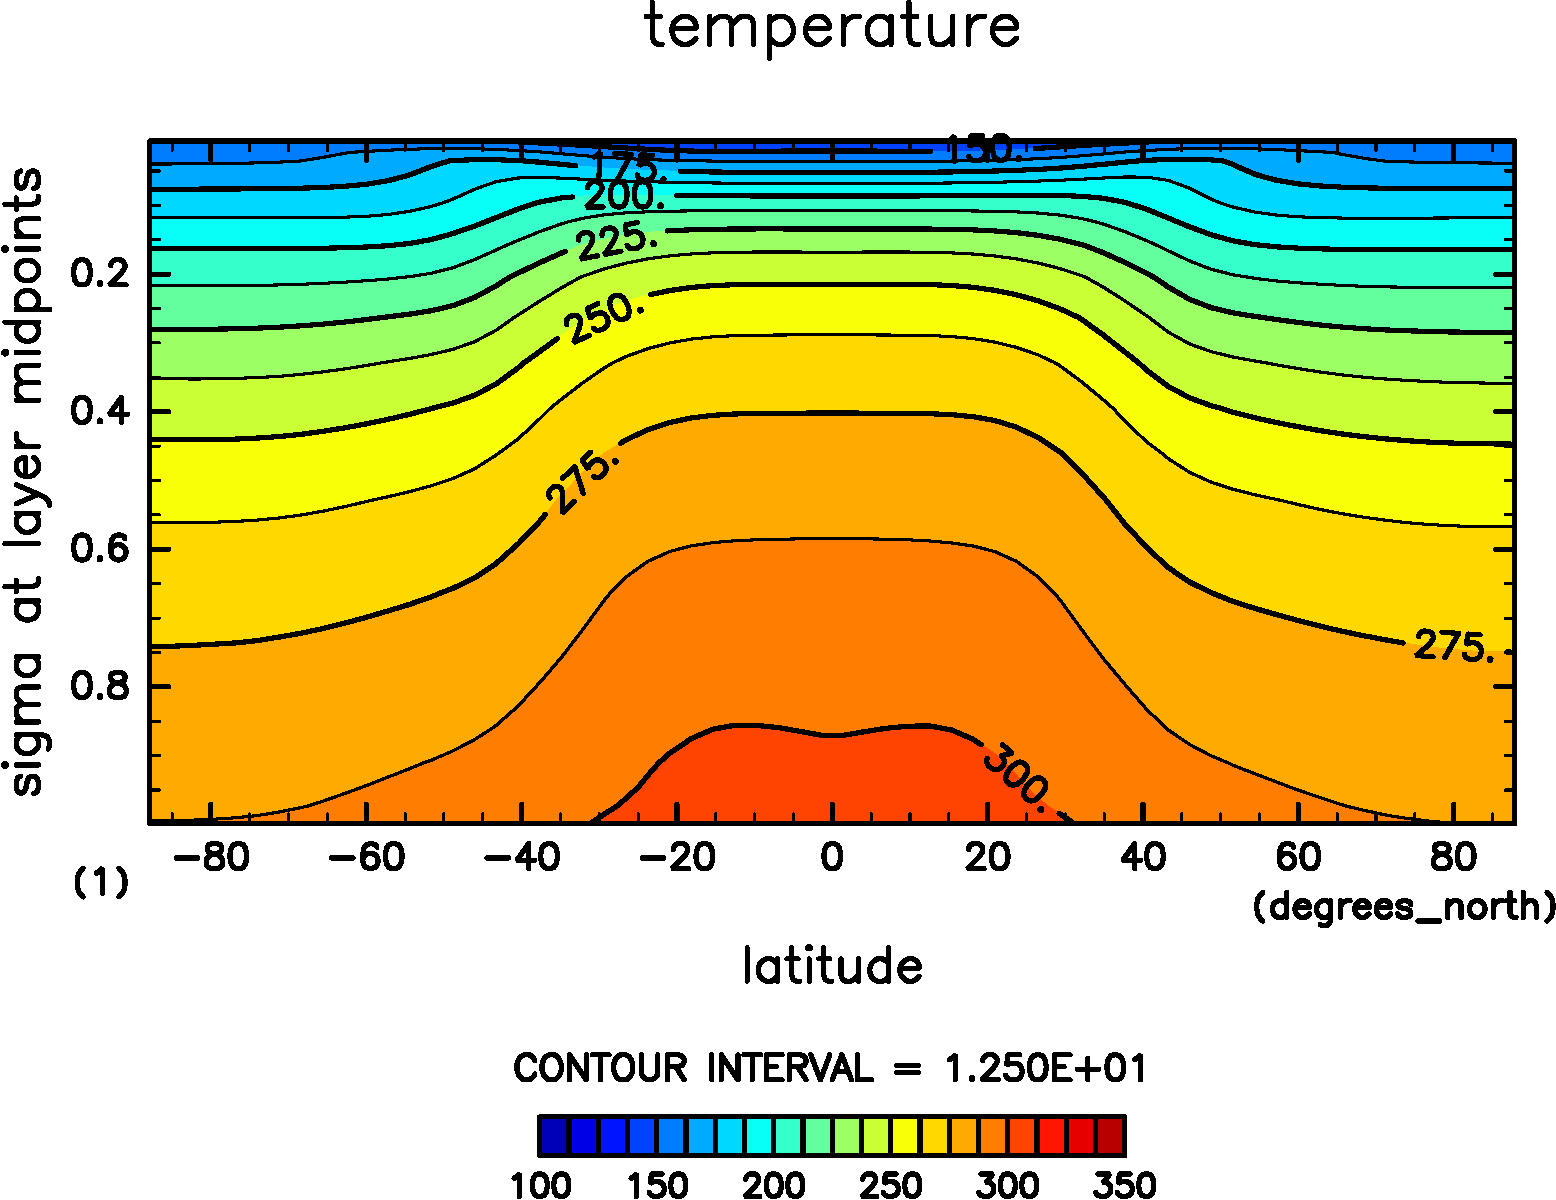
\includegraphics[width=\columnwidth]{S1600/Temp,time=3650:4015-crop-rotate.pdf}
		\caption{気温分布}\label{S1600気温分布}
	\end{subfigure}
	\begin{subfigure}{.4\textwidth}
		\centering
		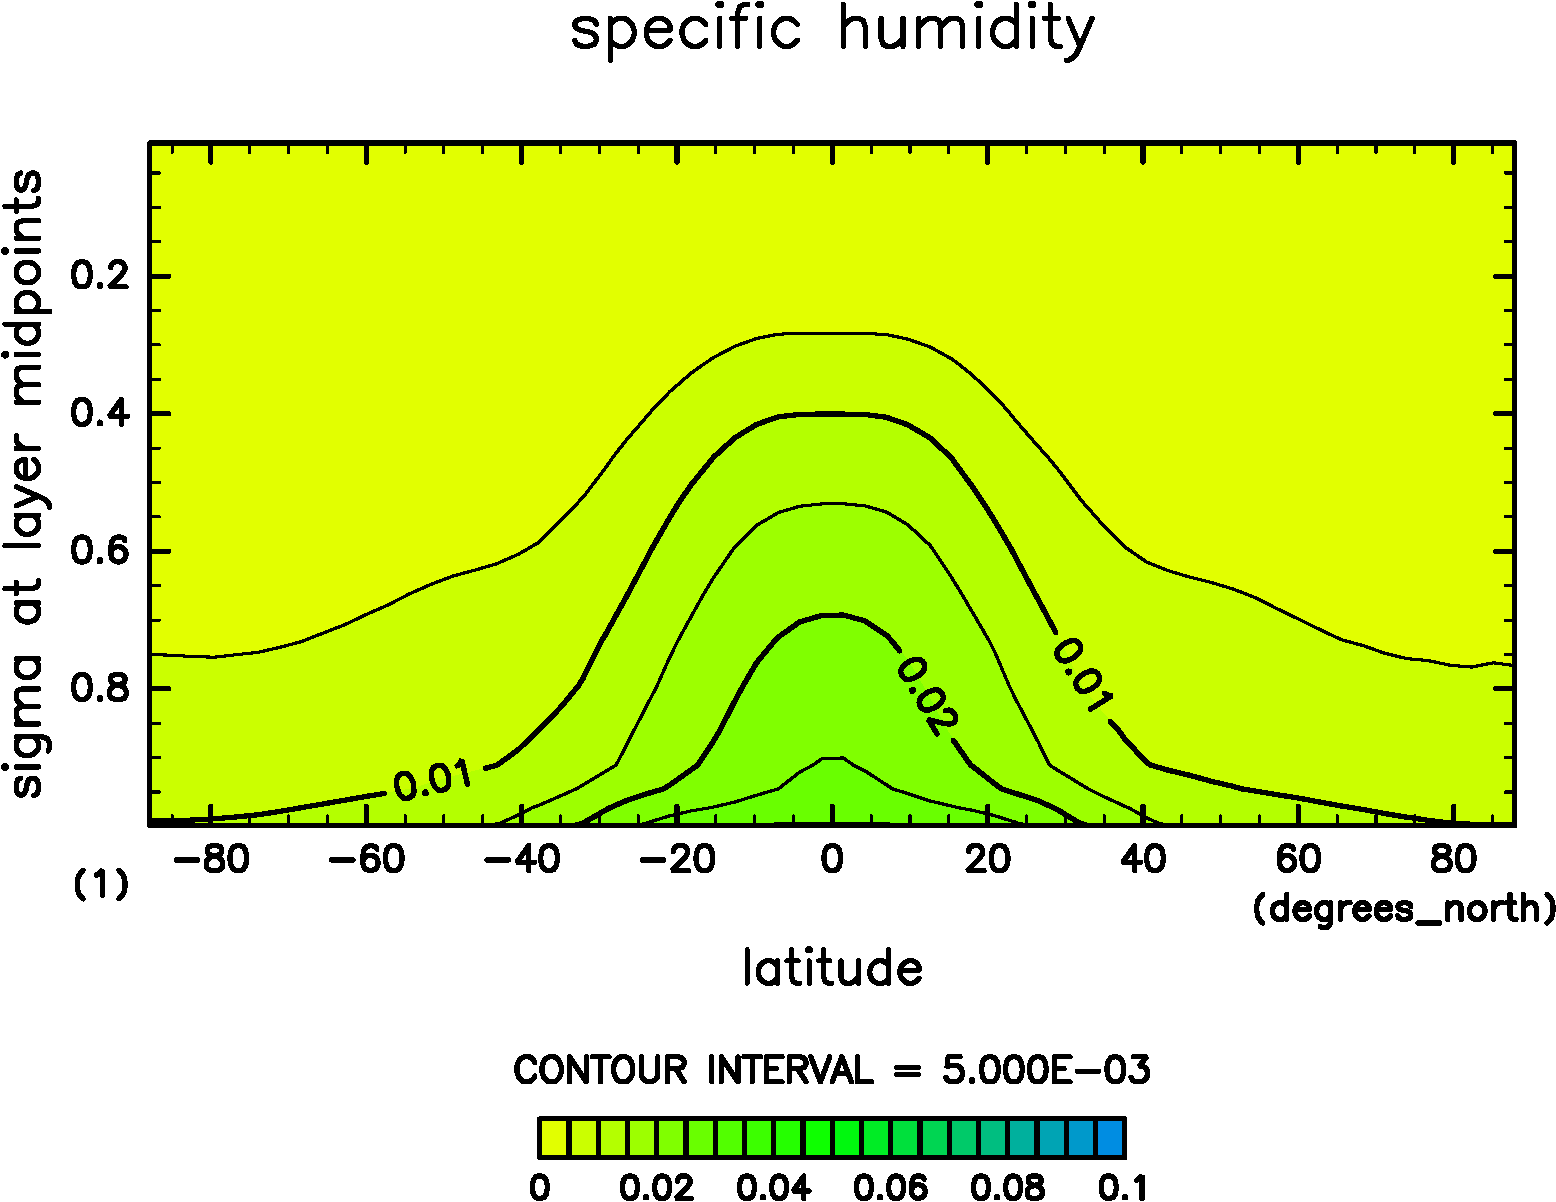
\includegraphics[width=\columnwidth]{S1600/QH2OVap,time=3650:4015-crop-rotate.pdf}
		\caption{比湿}\label{S1600比湿}
	\end{subfigure}
	\begin{subfigure}{.4\textwidth}
		\centering
		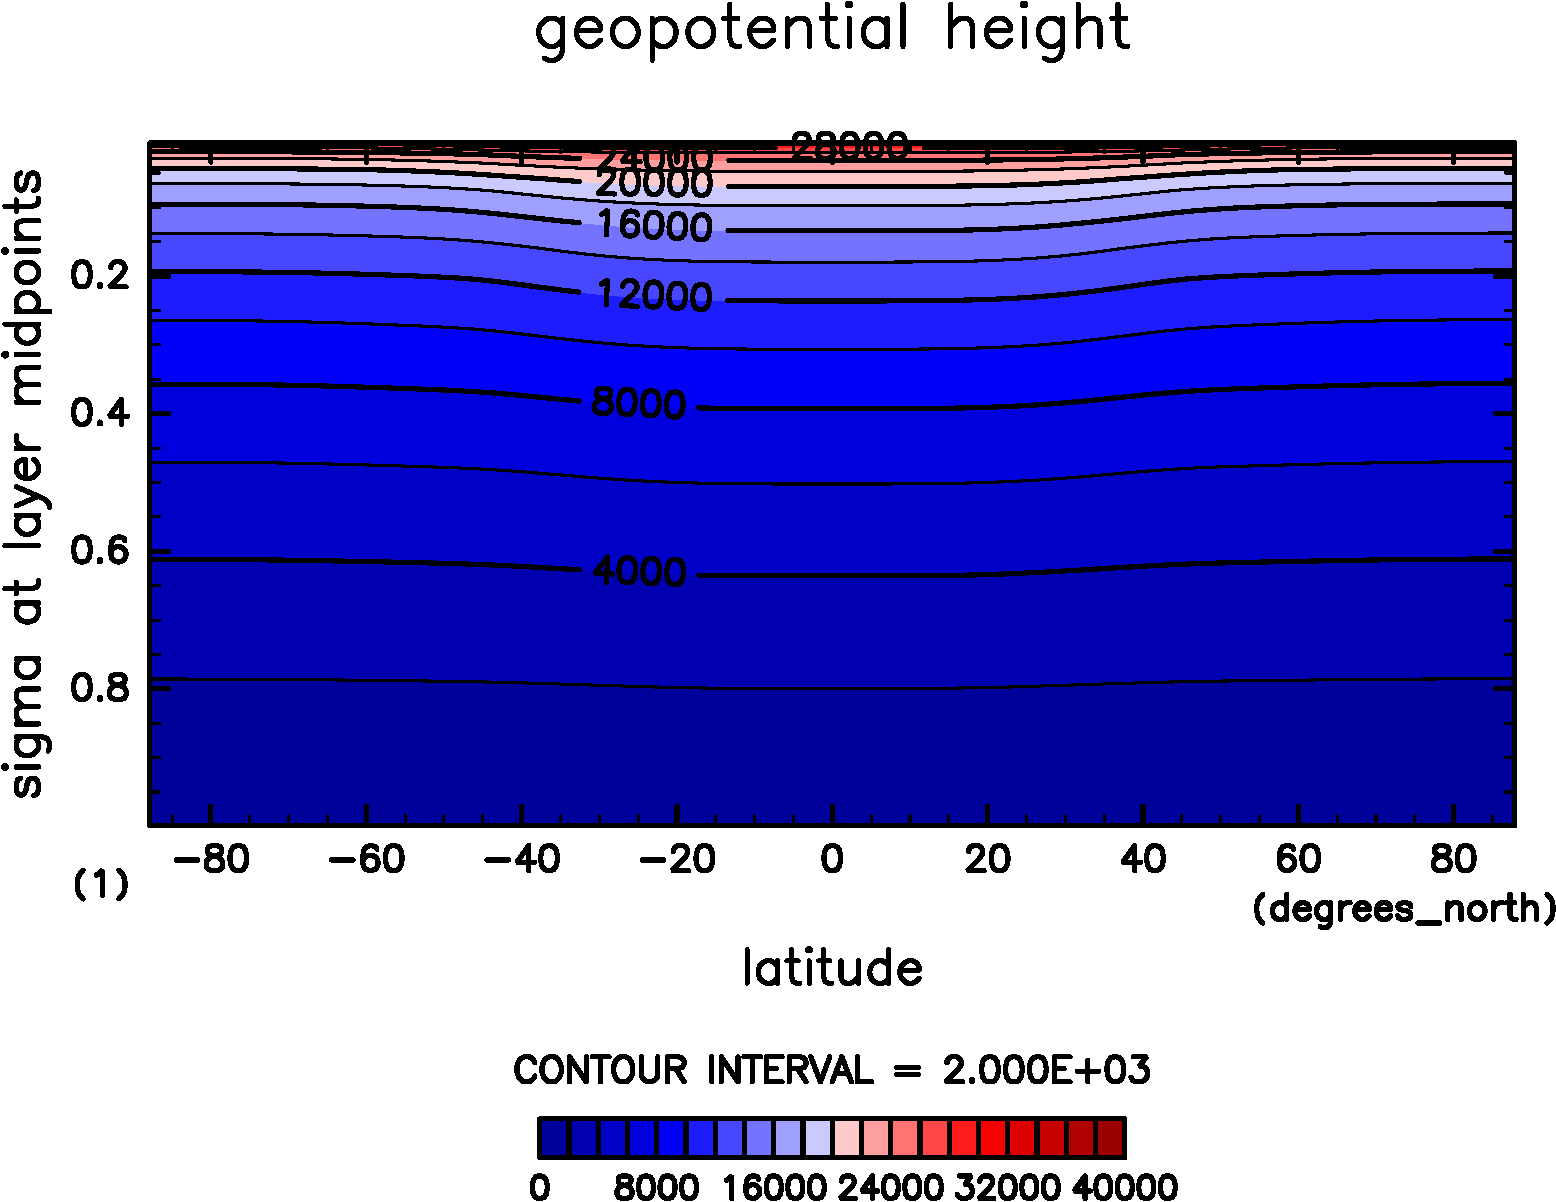
\includegraphics[width=\columnwidth]{S1600/Height,time=3650:4015-crop-rotate.pdf}
		\caption{ジオポテンシャル高度}\label{S1600ジオポテンシャル高度}
	\end{subfigure}
	\caption{
		\(S=1600\hmu{W/m^2}\) の結果。11 年目の年平均値。
	}\label{S1600}
\end{figure}

\begin{figure}[t]
	\centering
	\begin{subfigure}{.4\textwidth}
		\centering
		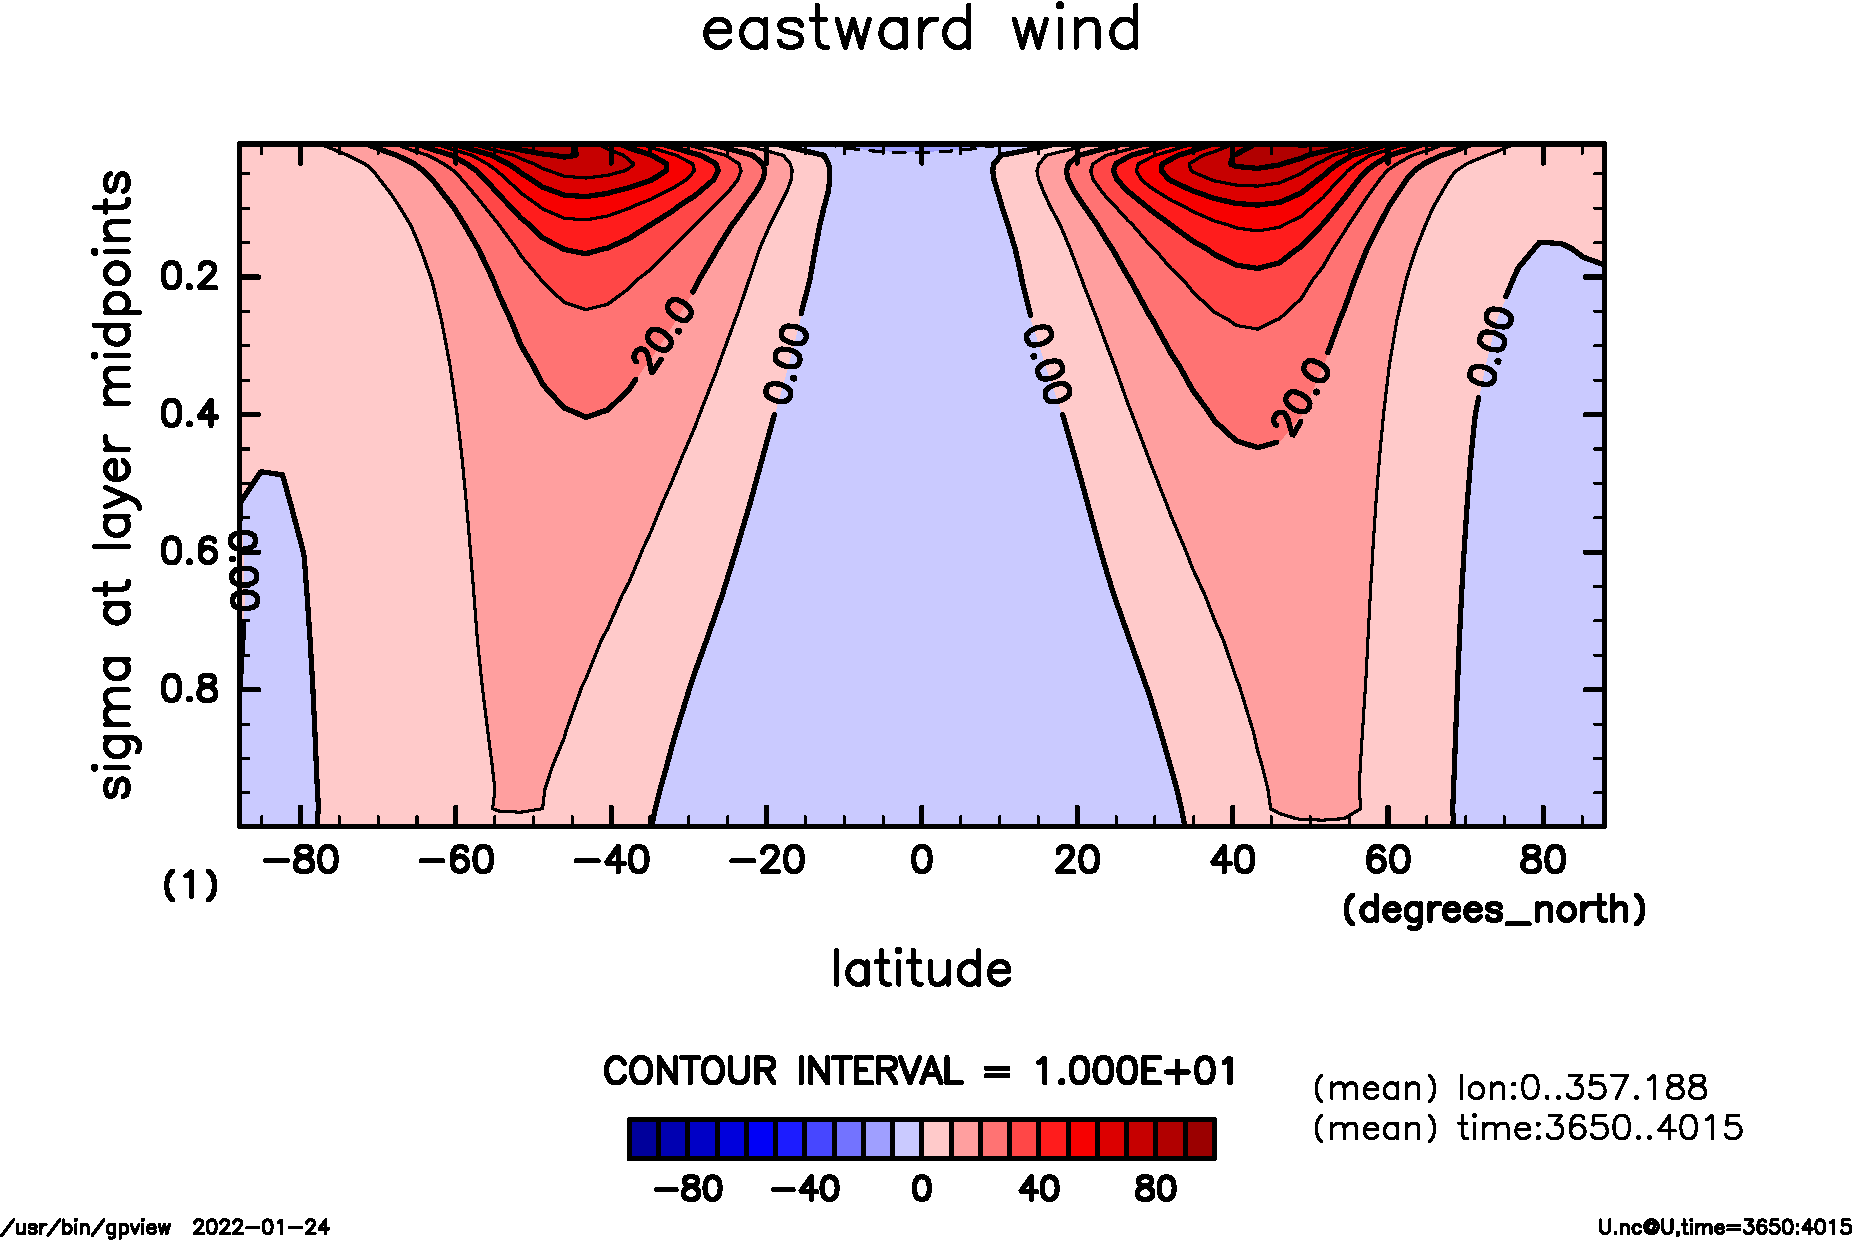
\includegraphics[width=\columnwidth]{S1800/U,time=3650:4015-crop-rotate.pdf}
		\caption{東西風}\label{S1800東西風}
	\end{subfigure}
	\begin{subfigure}{.4\textwidth}
		\centering
		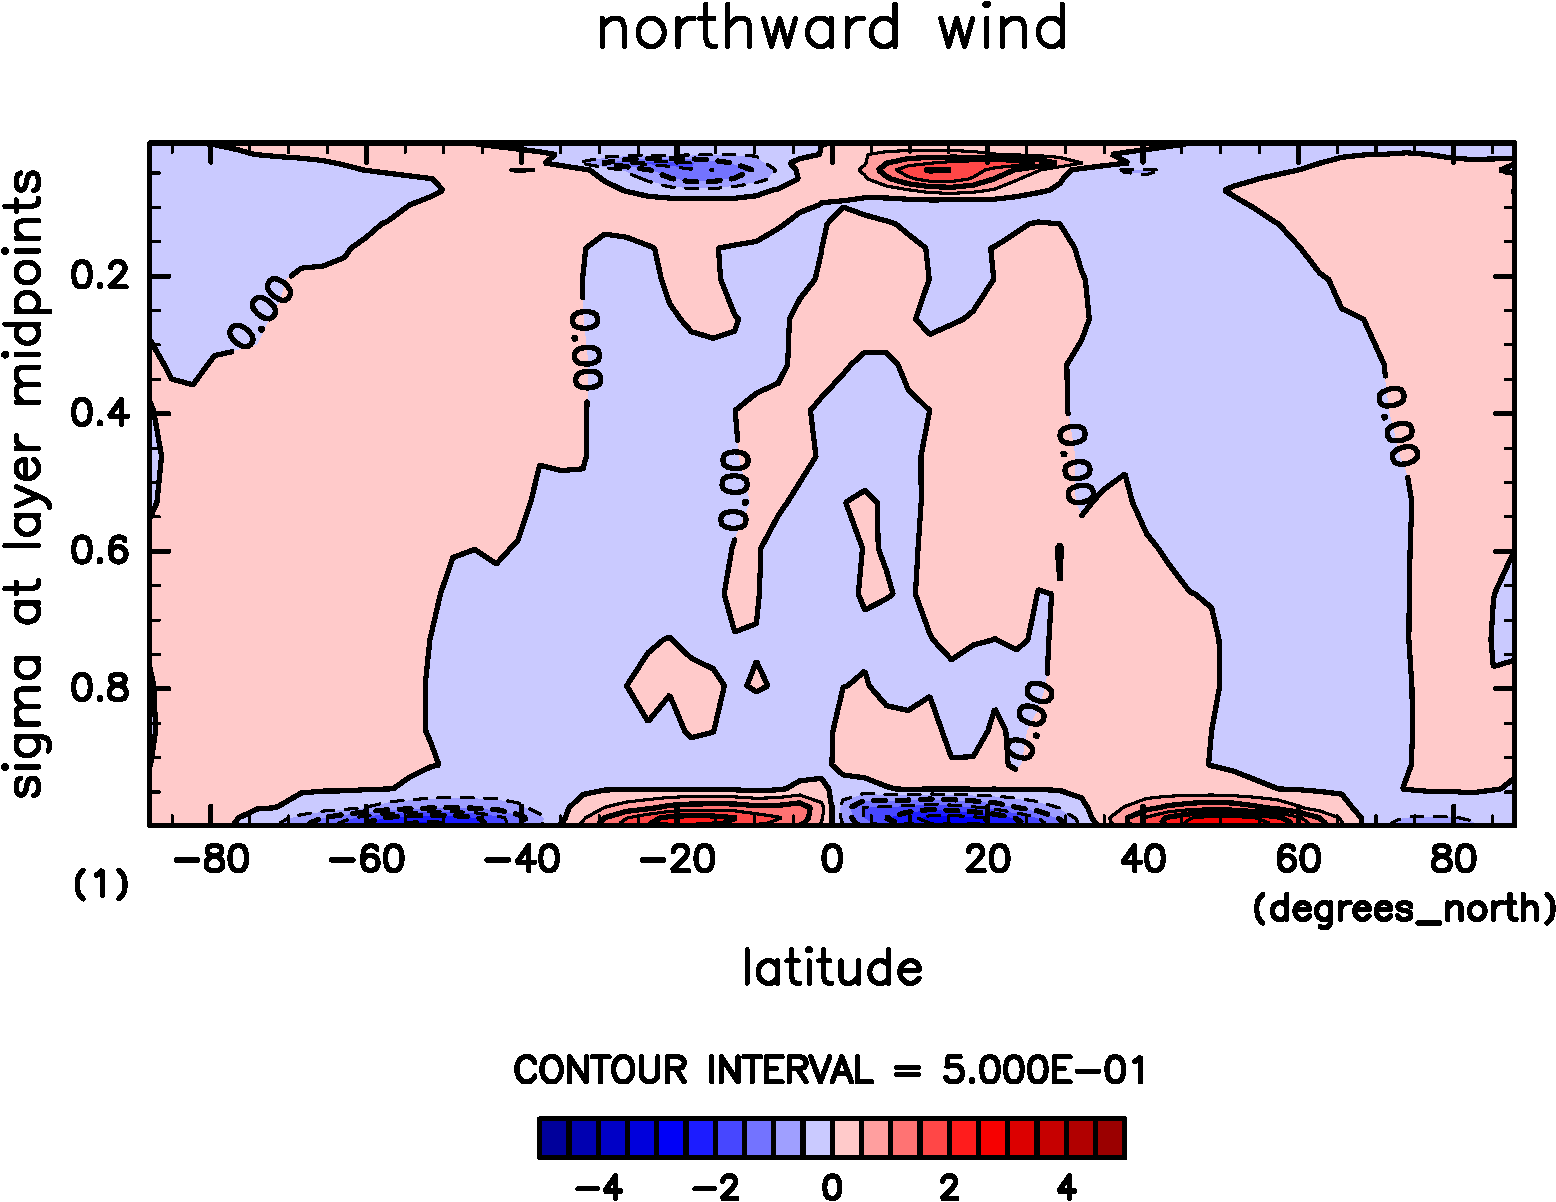
\includegraphics[width=\columnwidth]{S1800/V,time=3650:4015-crop-rotate.pdf}
		\caption{南北風}\label{S1800南北風}
	\end{subfigure}
	\begin{subfigure}{.4\textwidth}
		\centering
		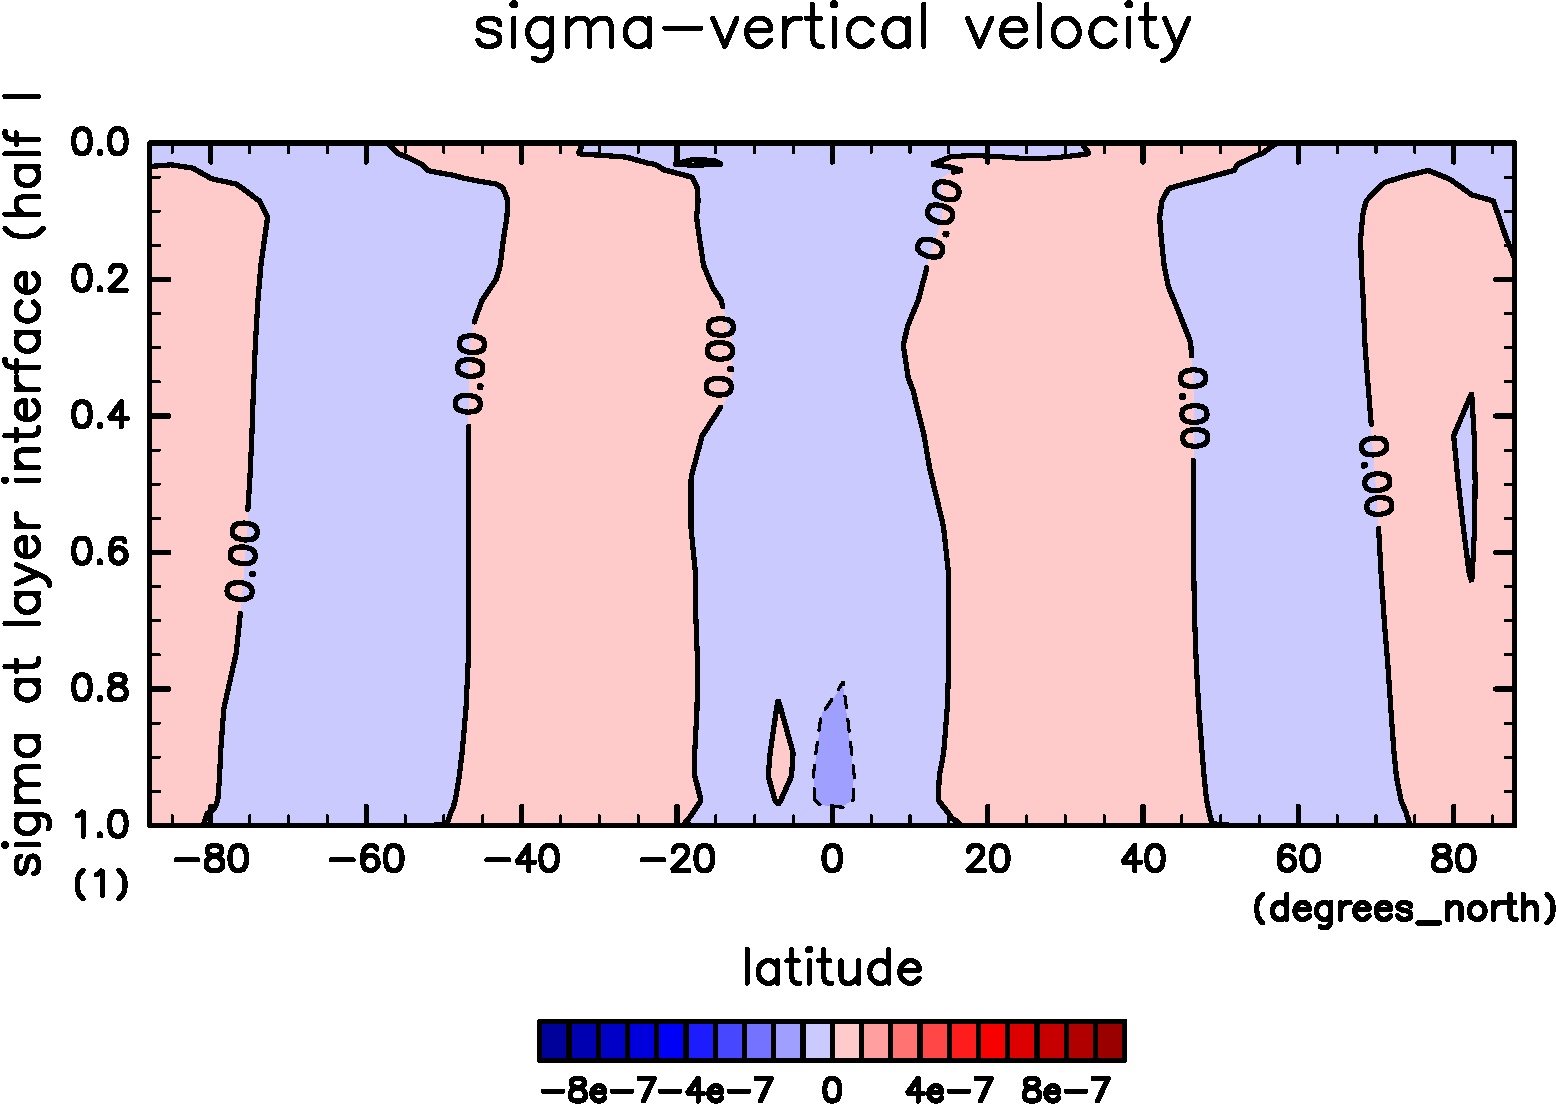
\includegraphics[width=\columnwidth]{S1800/SigDot,time=3650:4015-crop-rotate.pdf}
		\caption{鉛直風}\label{S1800鉛直風}
	\end{subfigure}
	\begin{subfigure}{.4\textwidth}
		\centering
		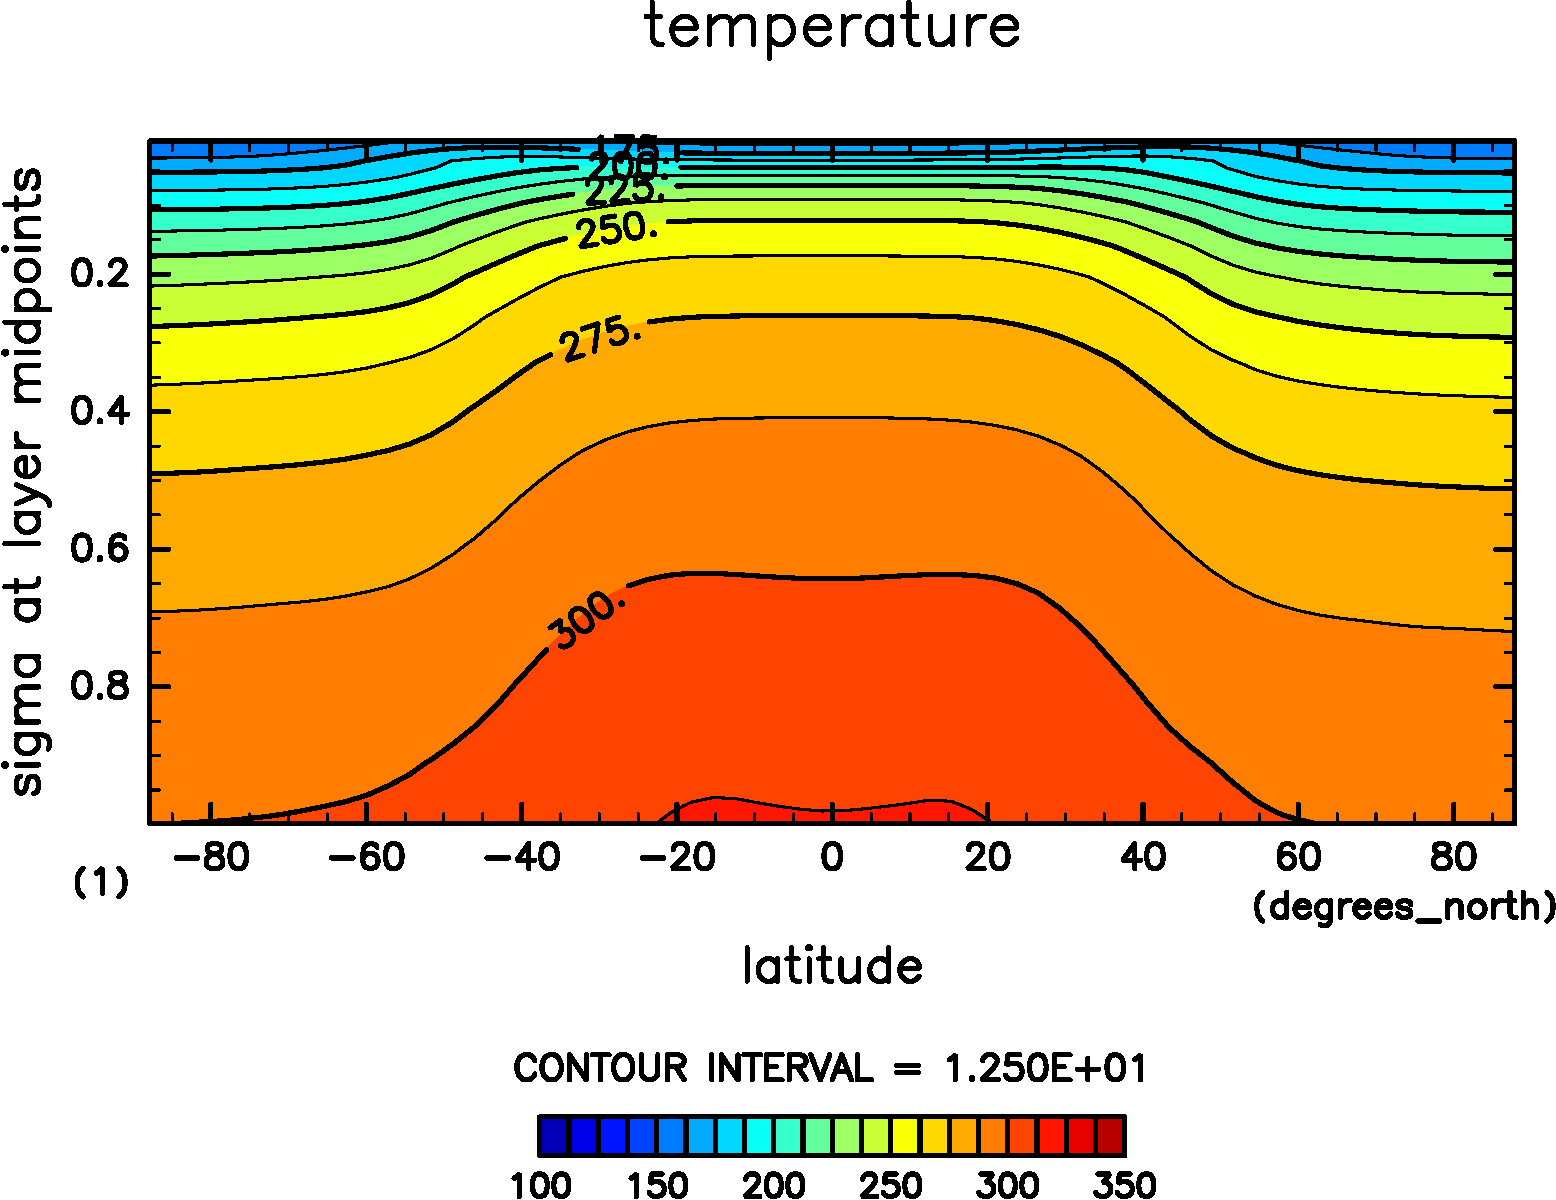
\includegraphics[width=\columnwidth]{S1800/Temp,time=3650:4015-crop-rotate.pdf}
		\caption{気温分布}\label{S1800気温分布}
	\end{subfigure}
	\begin{subfigure}{.4\textwidth}
		\centering
		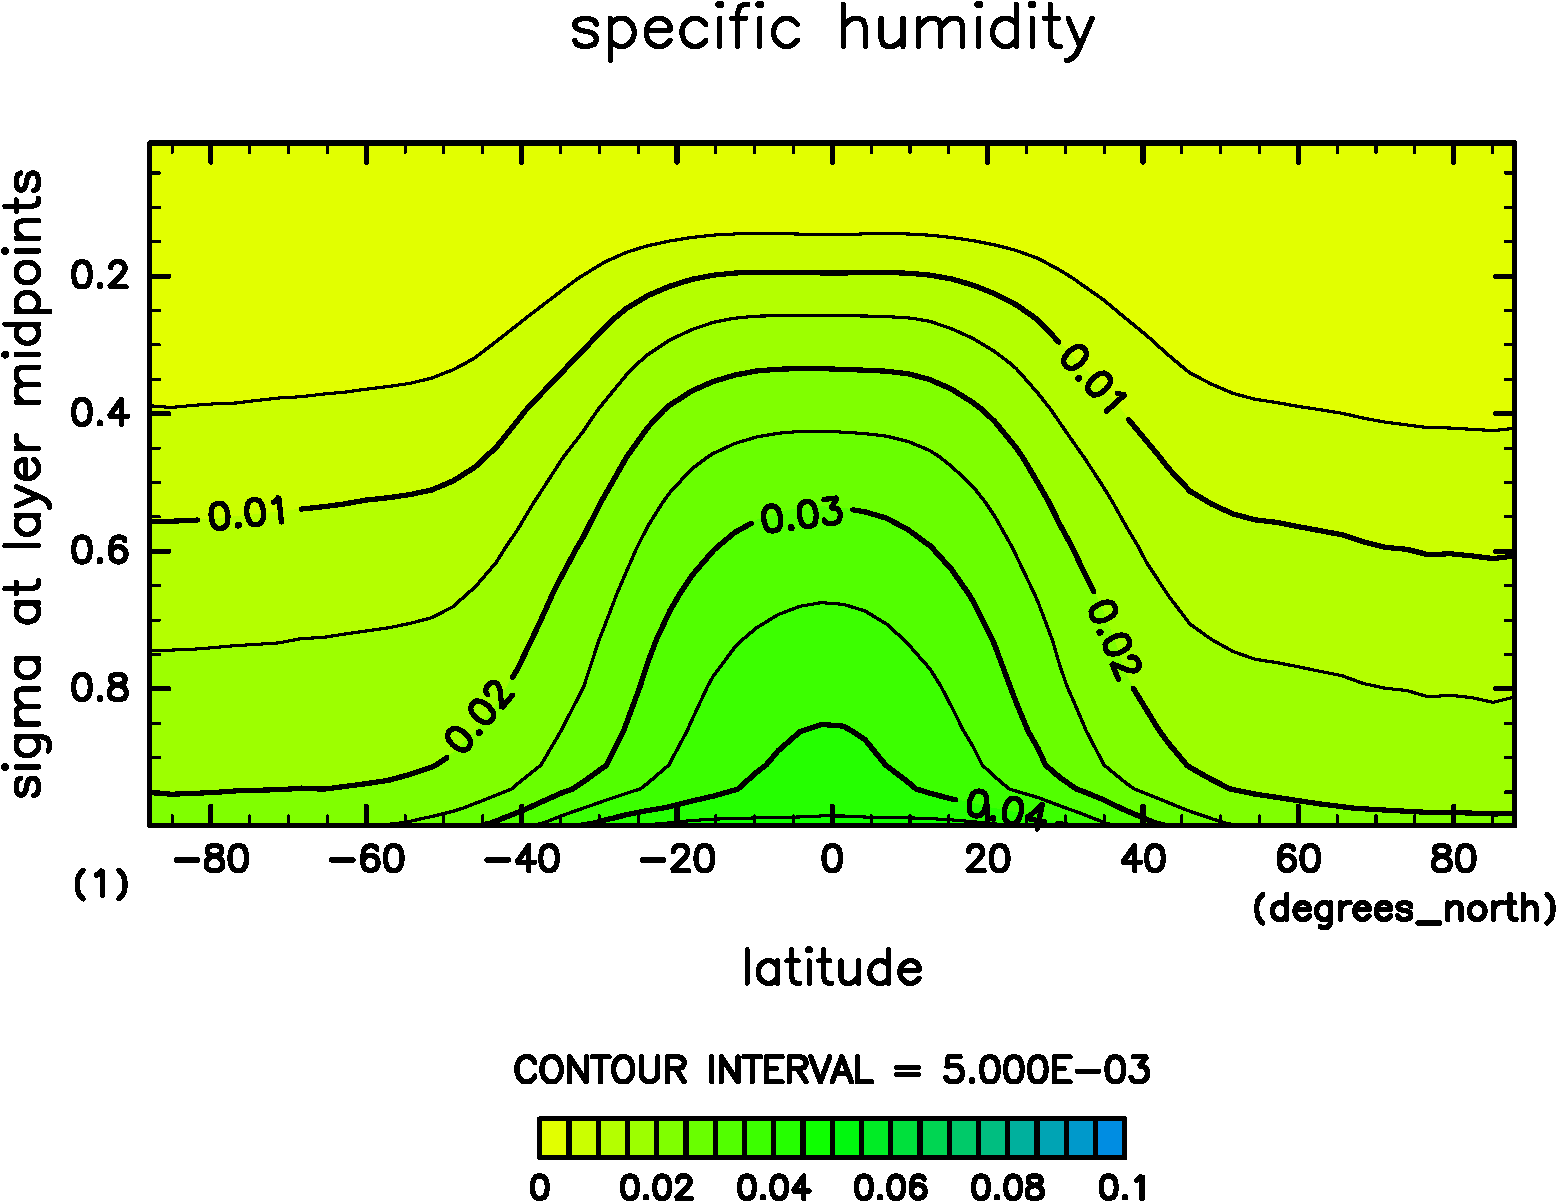
\includegraphics[width=\columnwidth]{S1800/QH2OVap,time=3650:4015-crop-rotate.pdf}
		\caption{比湿}\label{S1800比湿}
	\end{subfigure}
	\begin{subfigure}{.4\textwidth}
		\centering
		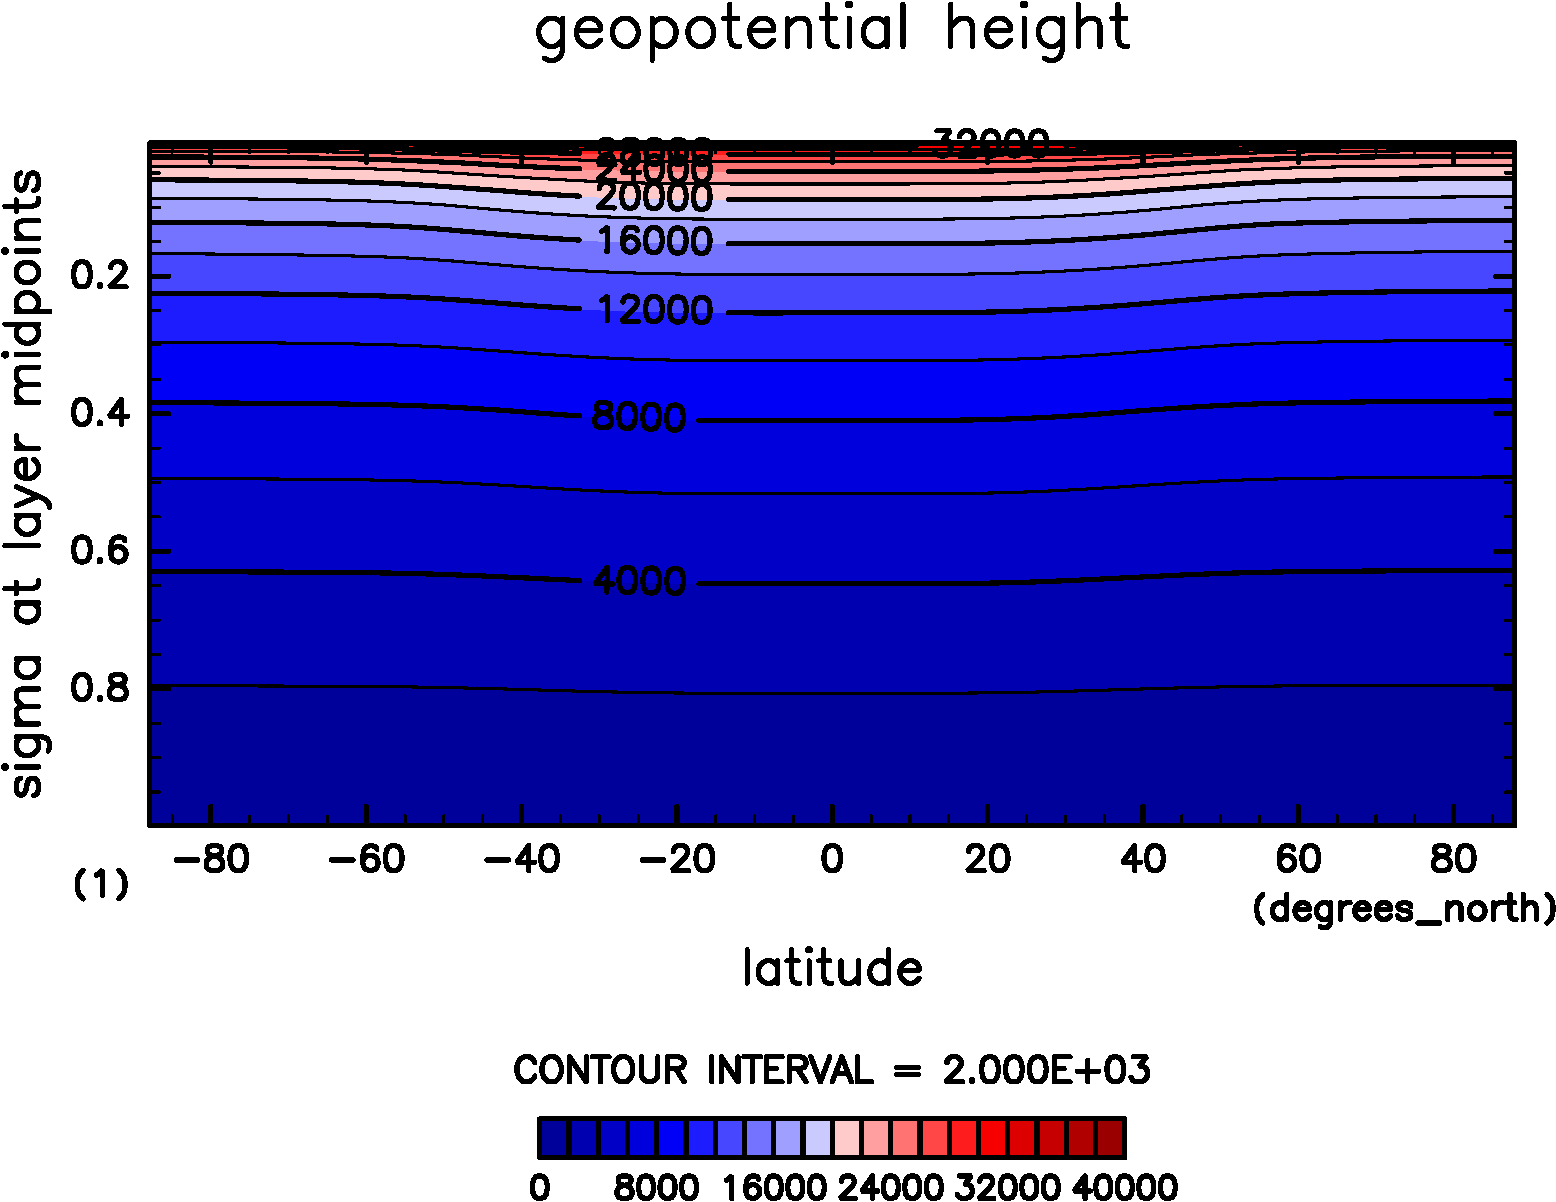
\includegraphics[width=\columnwidth]{S1800/Height,time=3650:4015-crop-rotate.pdf}
		\caption{ジオポテンシャル高度}\label{S1800ジオポテンシャル高度}
	\end{subfigure}
	\caption{
		\(S=1800\hmu{W/m^2}\) の結果。11 年目の年平均値。
	}\label{S1800}
\end{figure}

\begin{figure}[t]
	\centering
	\begin{subfigure}{.4\textwidth}
		\centering
		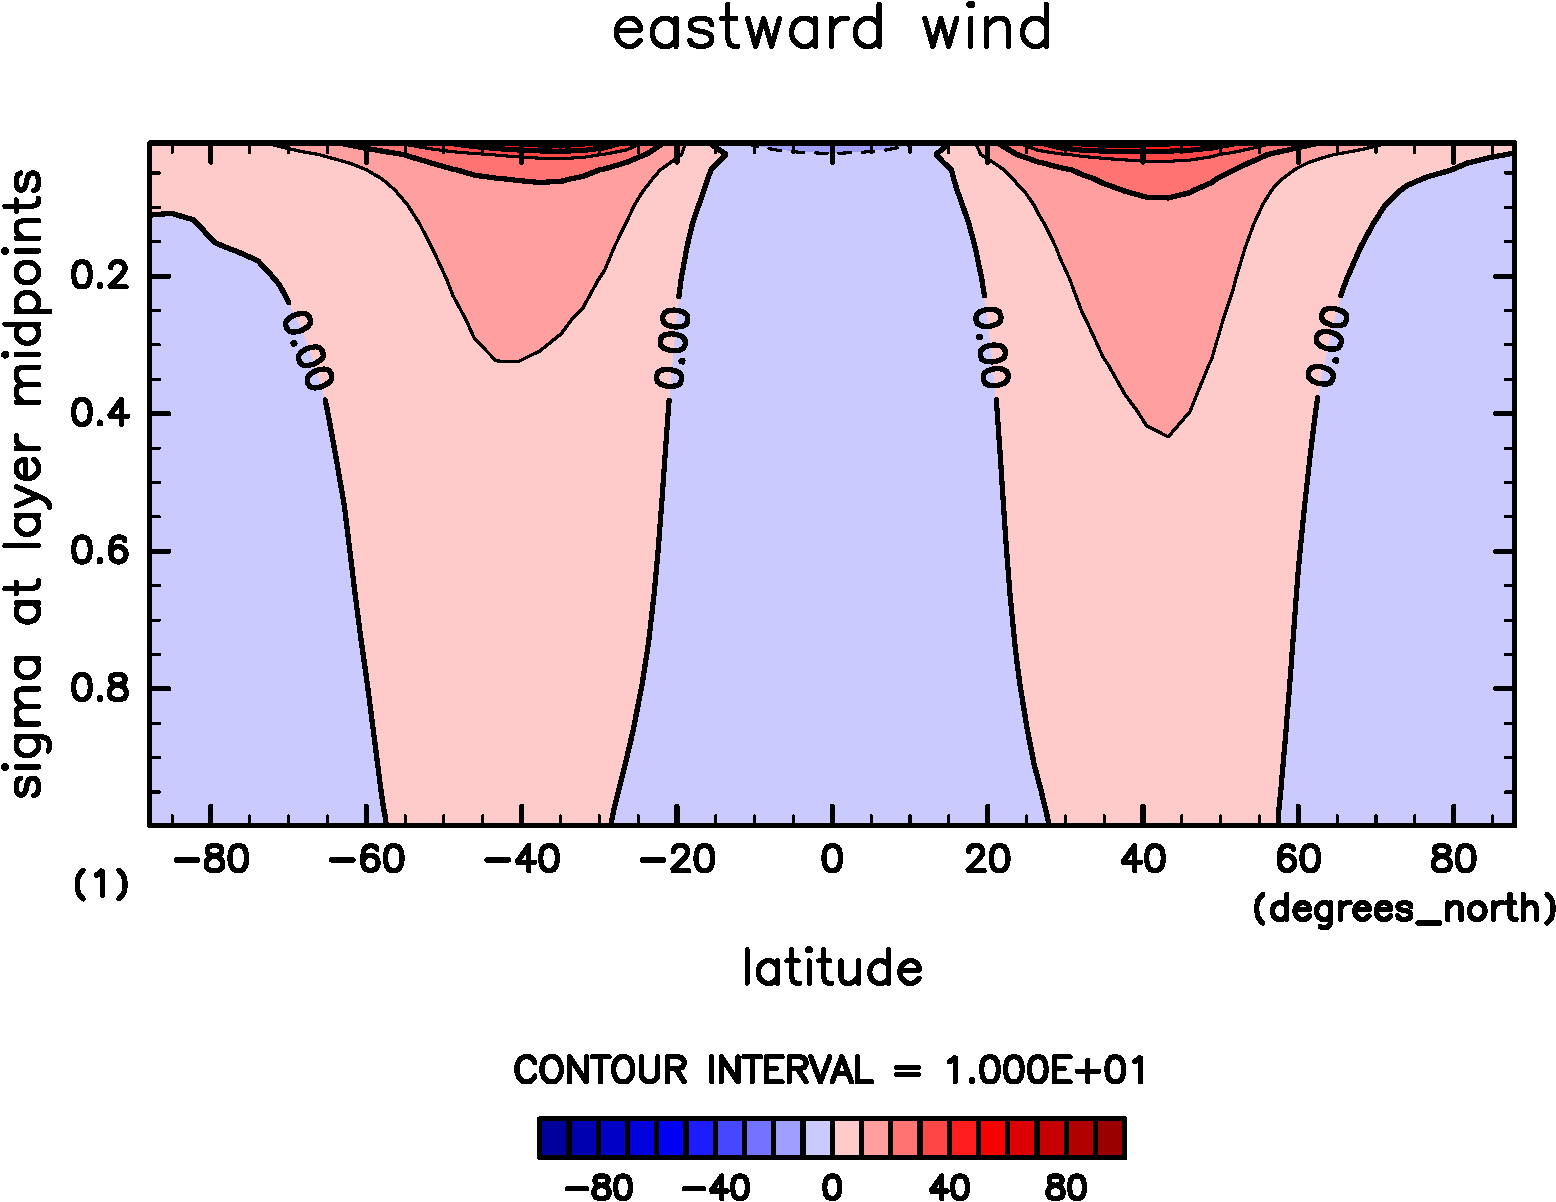
\includegraphics[width=\columnwidth]{S2000/U,time=7300:7665-crop-rotate.pdf}
		\caption{東西風}\label{S2000東西風}
	\end{subfigure}
	\begin{subfigure}{.4\textwidth}
		\centering
		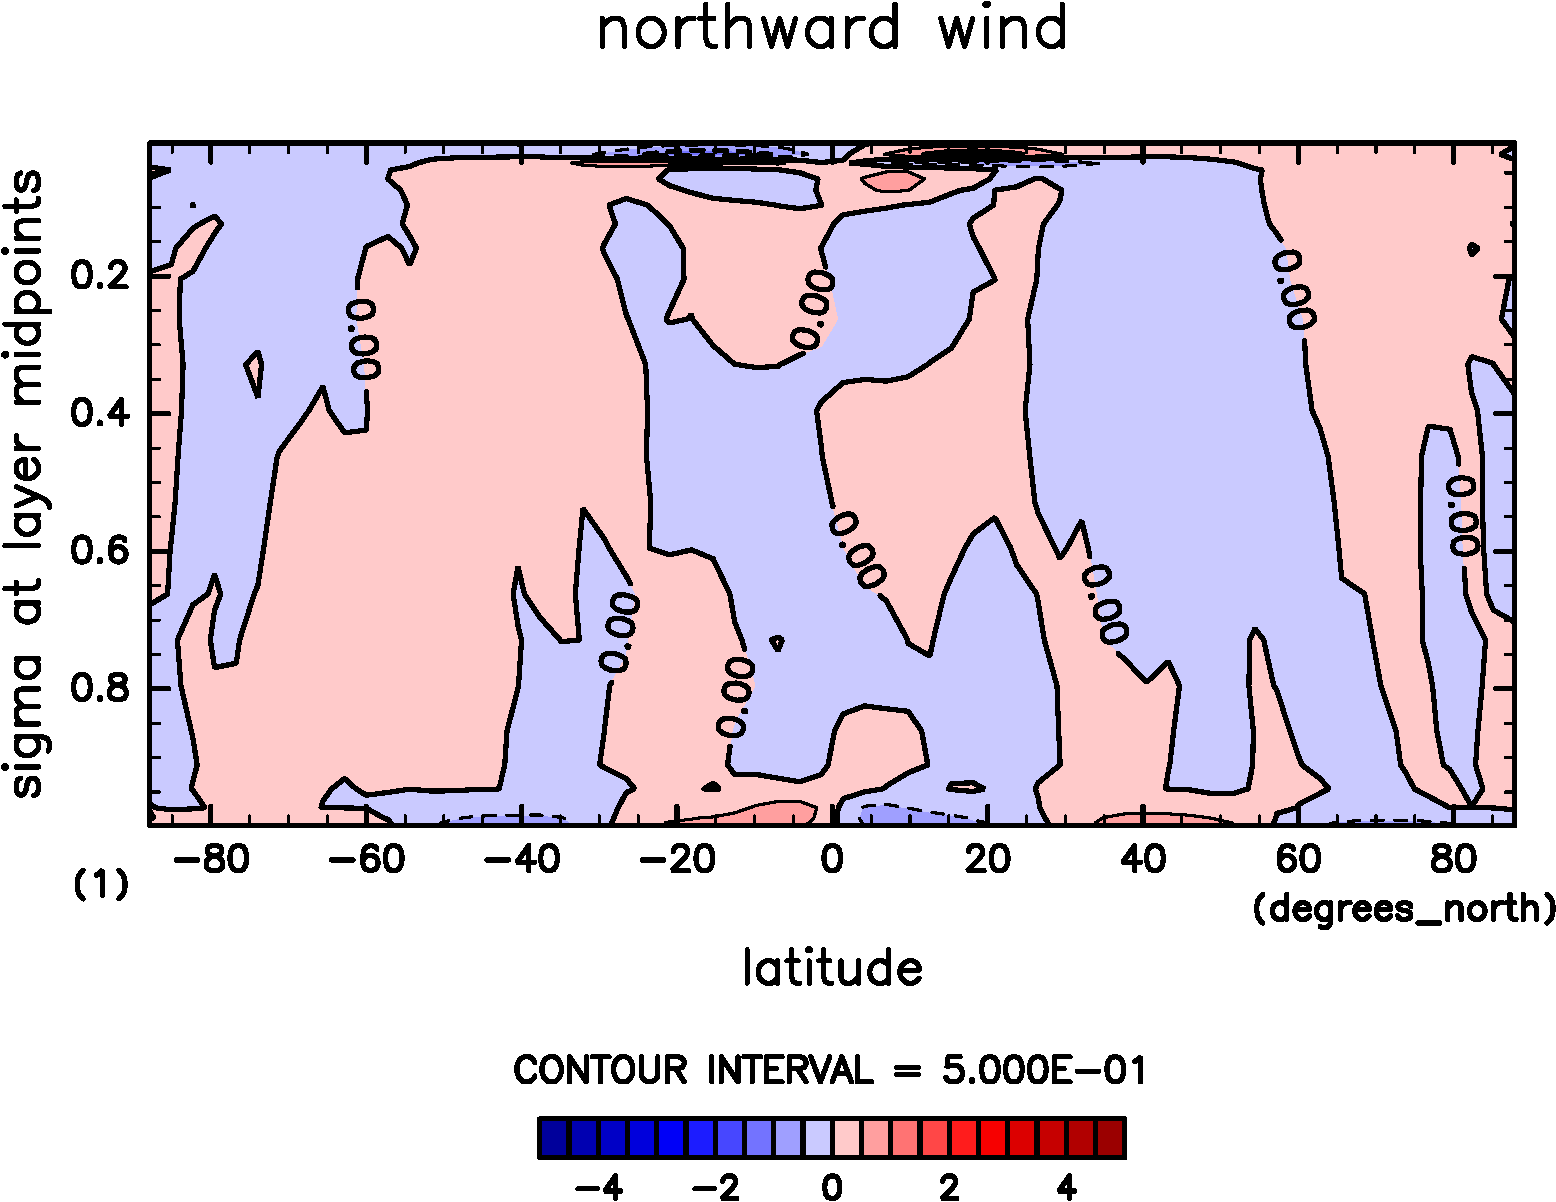
\includegraphics[width=\columnwidth]{S2000/V,time=7300:7665-crop-rotate.pdf}
		\caption{南北風}\label{S2000南北風}
	\end{subfigure}
	\begin{subfigure}{.4\textwidth}
		\centering
		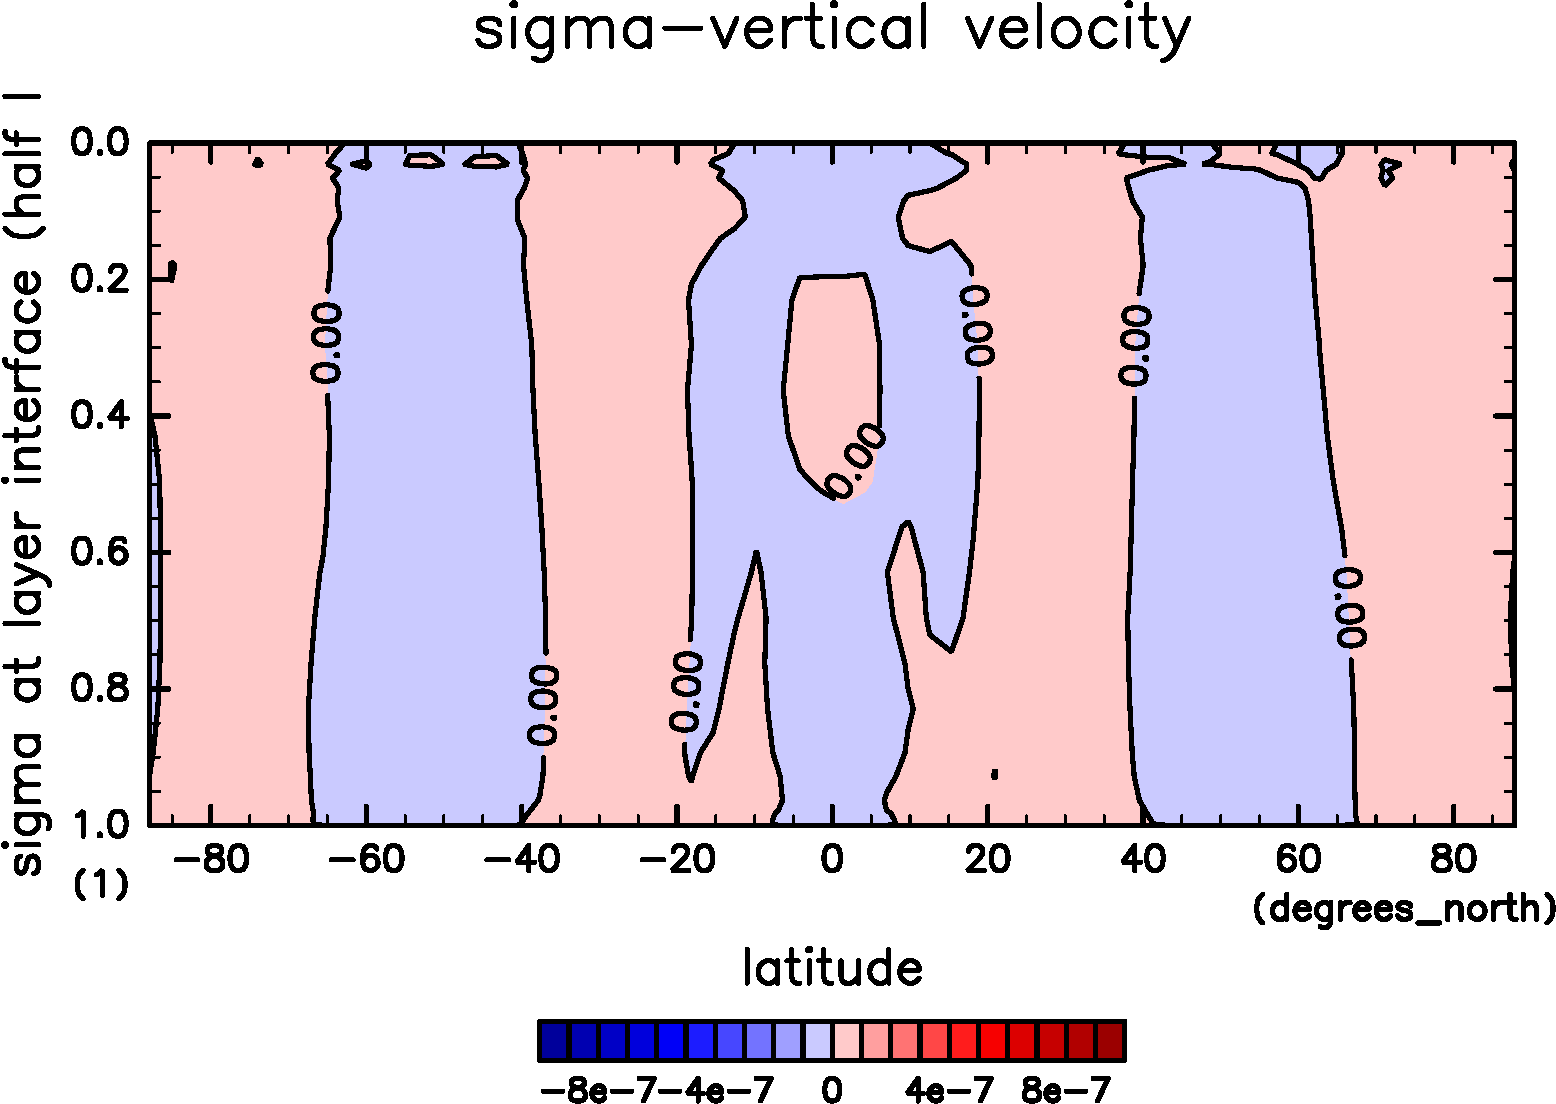
\includegraphics[width=\columnwidth]{S2000/SigDot,time=7300:7665-crop-rotate.pdf}
		\caption{鉛直風}\label{S2000鉛直風}
	\end{subfigure}
	\begin{subfigure}{.4\textwidth}
		\centering
		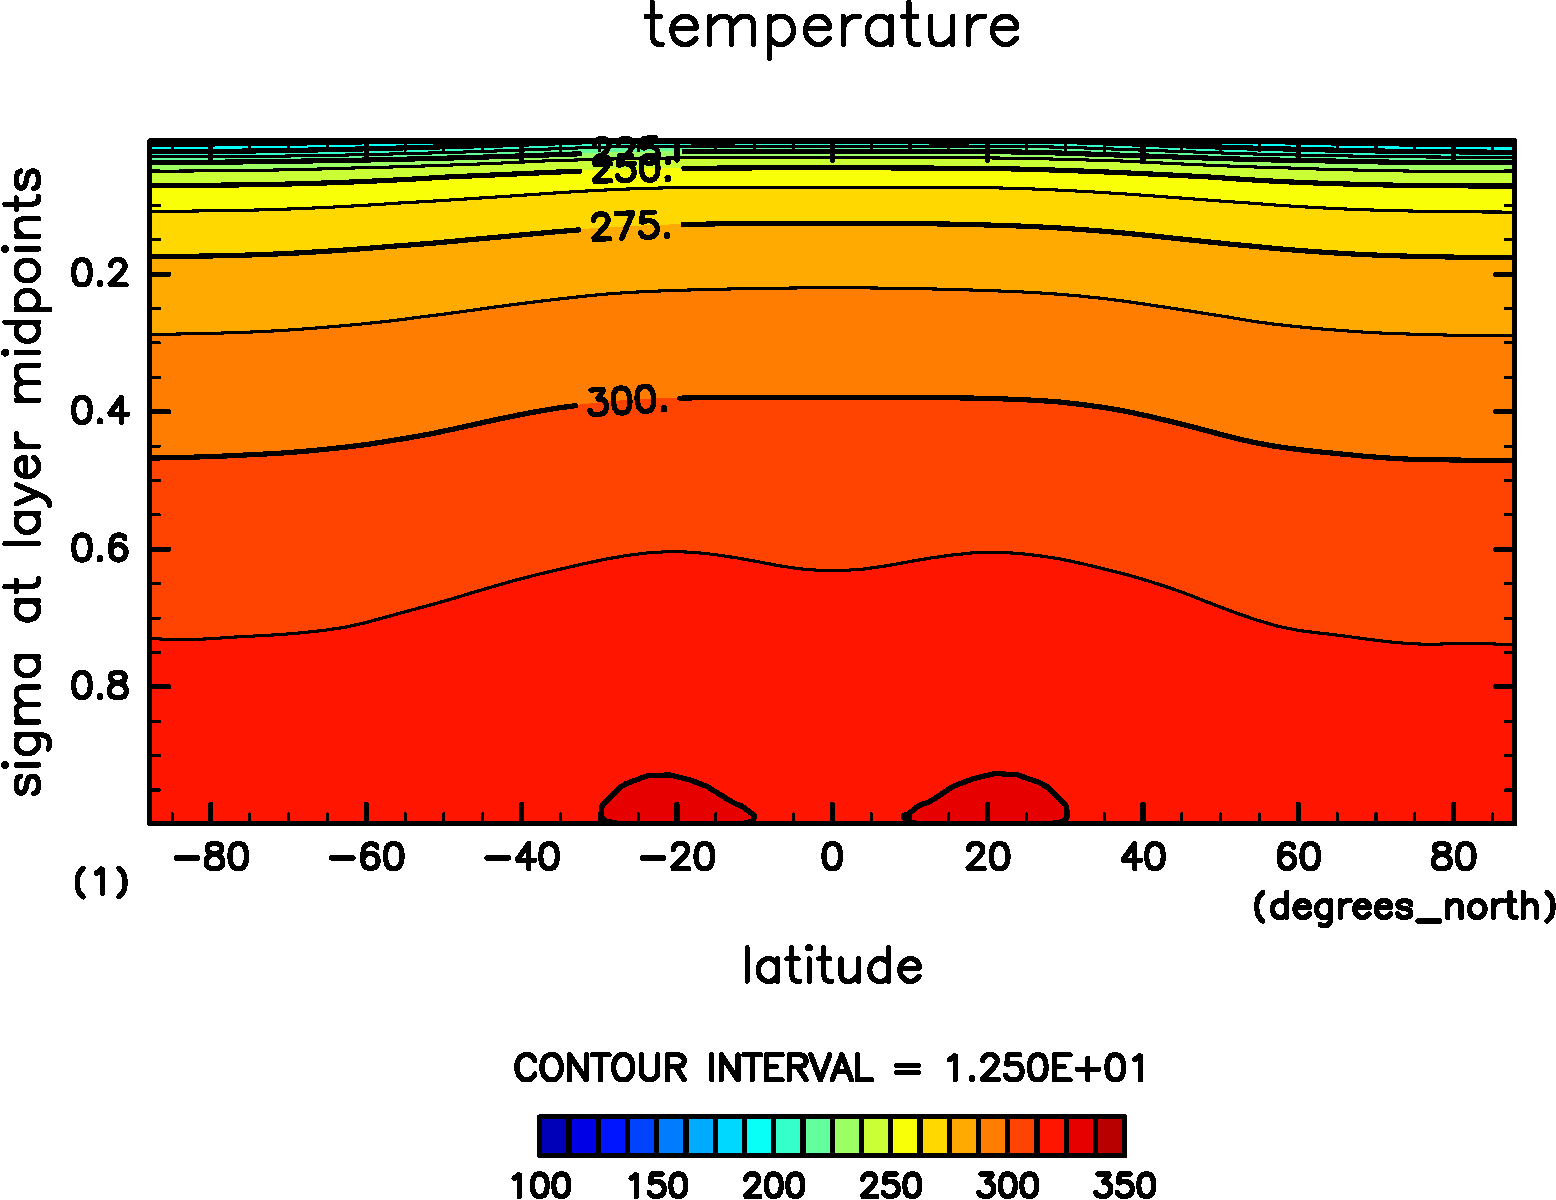
\includegraphics[width=\columnwidth]{S2000/Temp,time=7300:7665-crop-rotate.pdf}
		\caption{気温分布}\label{S2000気温分布}
	\end{subfigure}
	\begin{subfigure}{.4\textwidth}
		\centering
		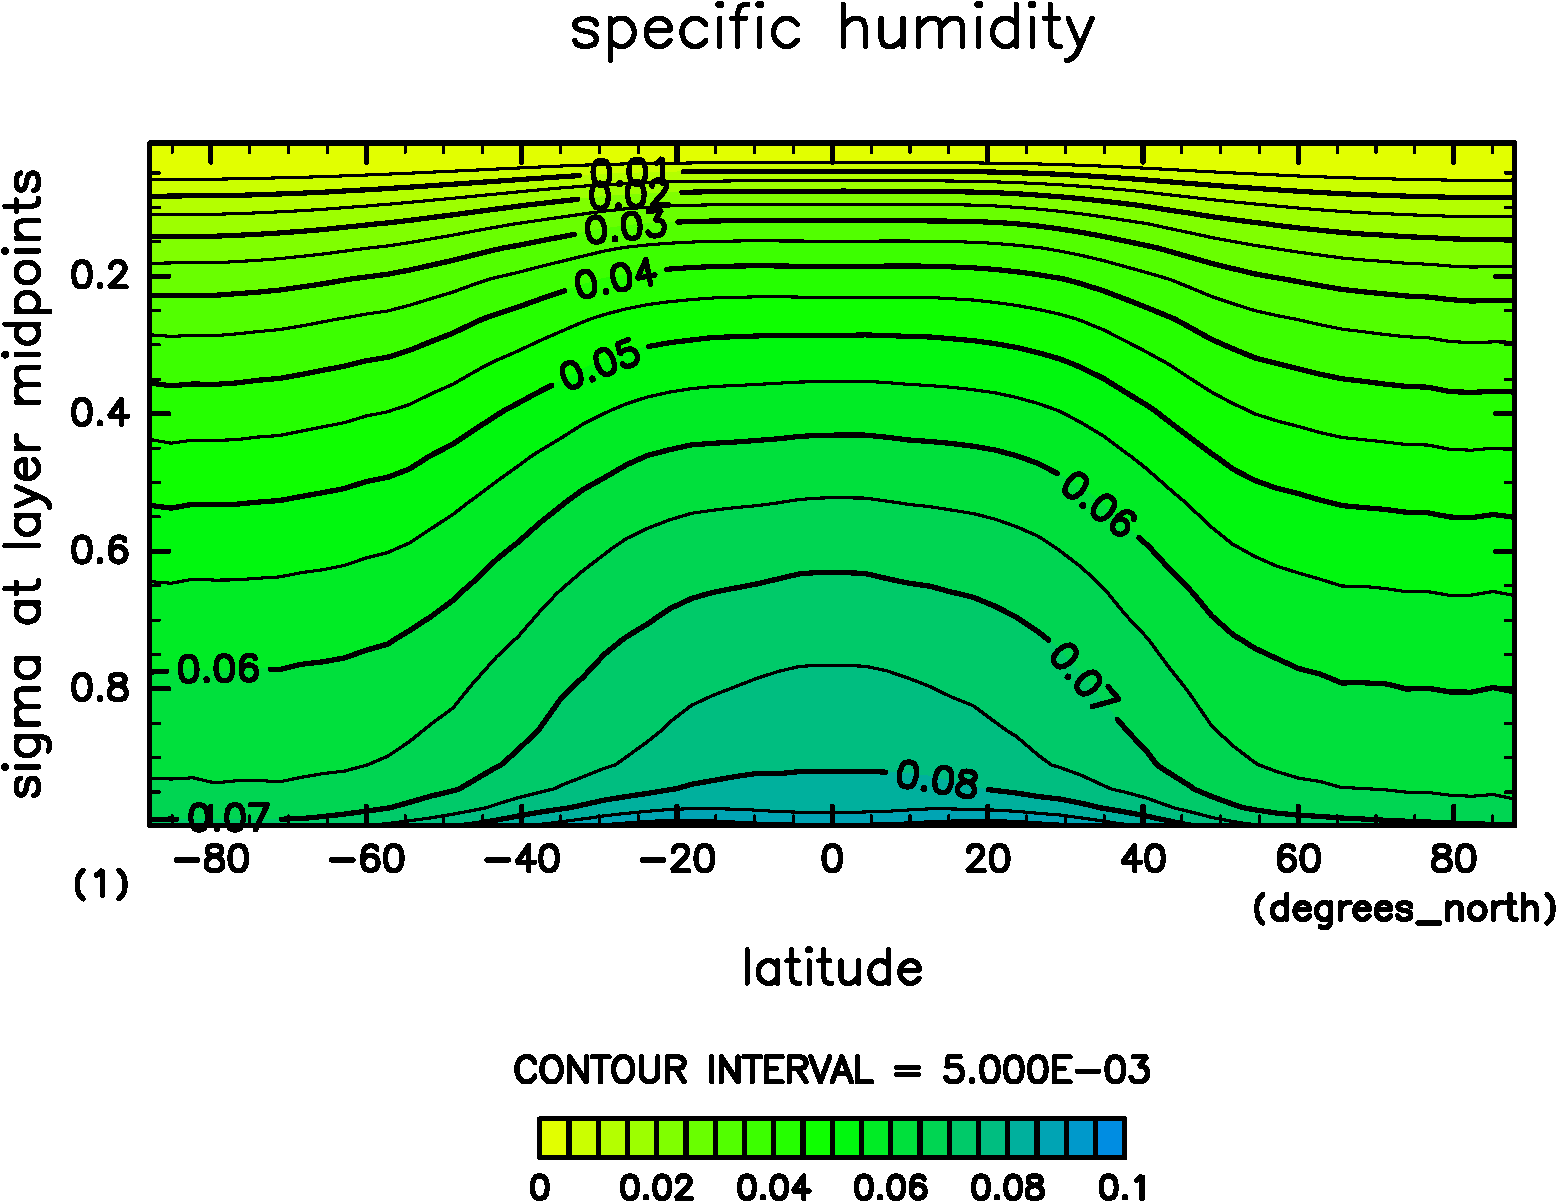
\includegraphics[width=\columnwidth]{S2000/QH2OVap,time=7300:7665-crop-rotate.pdf}
		\caption{比湿}\label{S2000比湿}
	\end{subfigure}
	\begin{subfigure}{.4\textwidth}
		\centering
		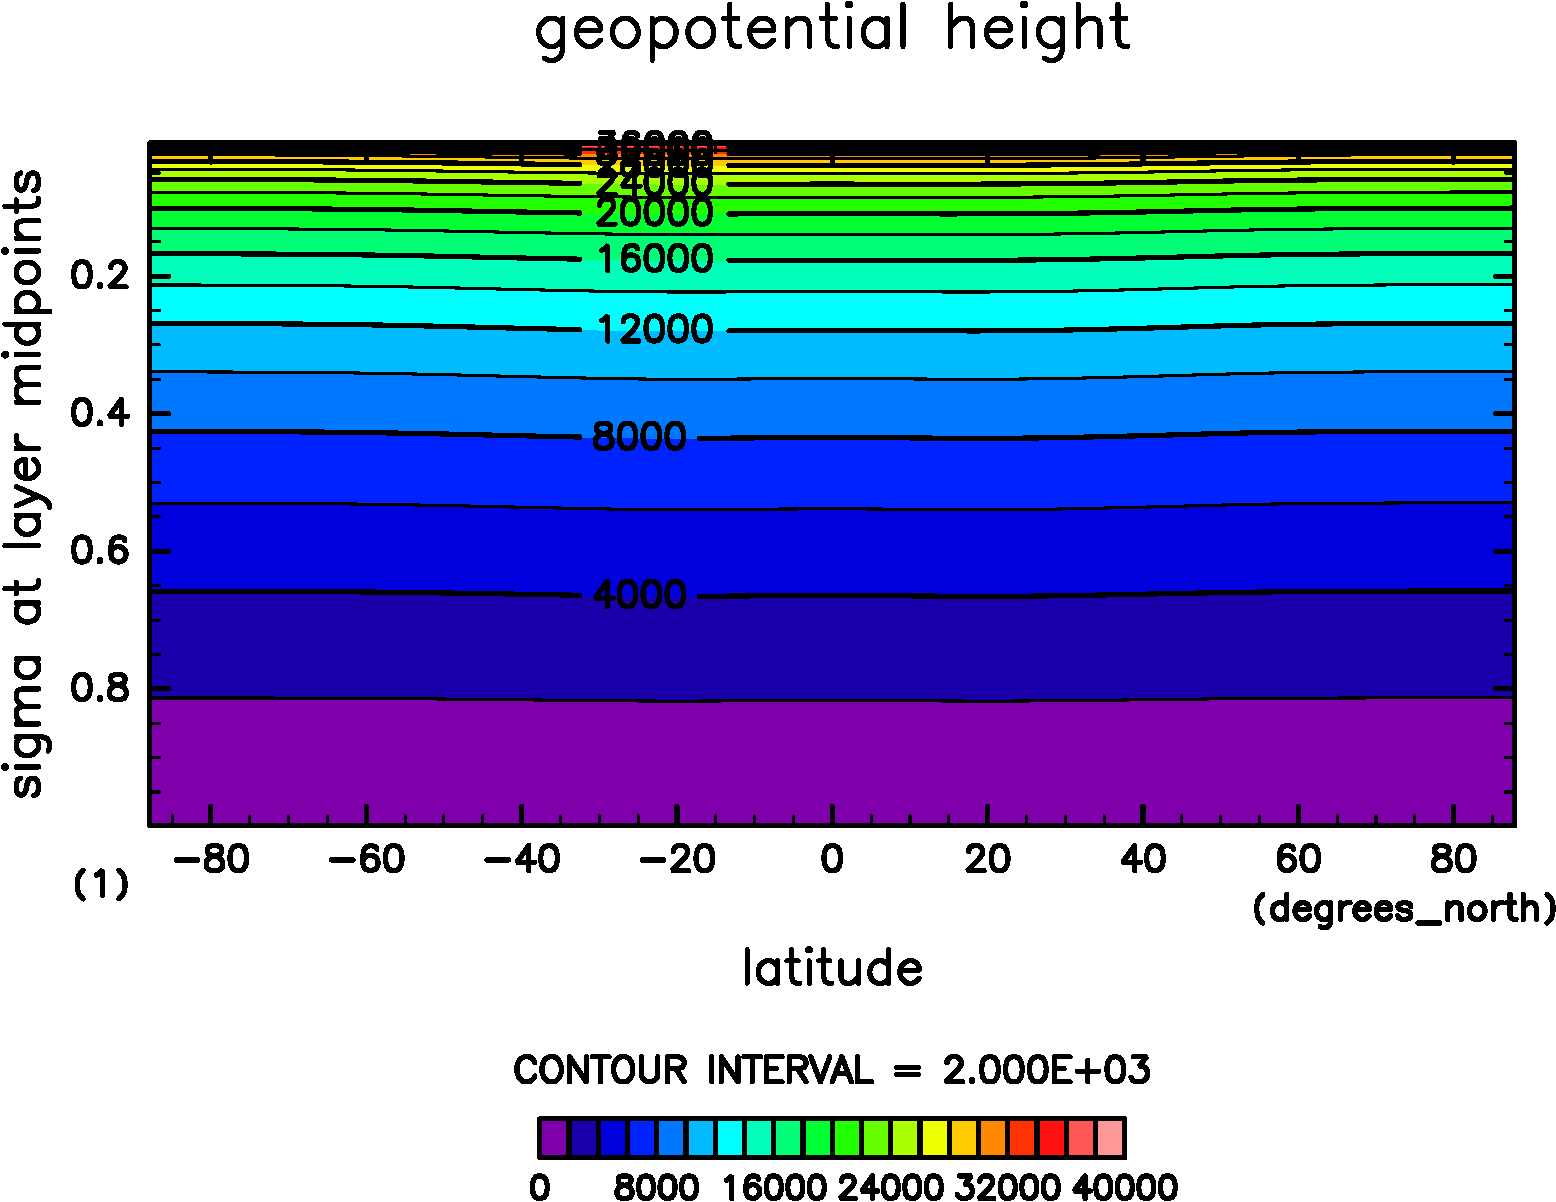
\includegraphics[width=\columnwidth]{S2000/Height,time=7300:7665-crop-rotate.pdf}
		\caption{ジオポテンシャル高度}\label{S2000ジオポテンシャル高度}
	\end{subfigure}
	\caption{
		\(S=2000\hmu{W/m^2}\) の結果。31 年目の年平均値。
	}\label{S2000}
\end{figure}

\section{南北熱輸送の太陽定数依存性}

南北熱輸送に関して考察する。南北熱輸送は、潜熱によるもの \(F_L\) と、
乾燥静的エネルギー \(F_D\) によるものとに分類できる。そして、\(F_L\) と
\(F_D\) の和が全熱輸送量 \(F_T\) になる。乾燥静的エネルギーはエンタルピー
とジオポテンシャルの和であるから、それぞれ式で表せば以下のようになる。

\begin{gather}
	F_L=\int_{p_s}^0 Lqv\,dp=\int_1^0 Lqvp_s\,d\sigma,\\
	F_D=\int_{p_s}^0 (c_{pn}T+gz)v\,dp=\int_1^0 (c_{pn}T+gz)vp_s\,d\sigma,\\
	F_T=F_L+F_D.
\end{gather}

図 \ref{EnFlx} に東西平均・時間平均をした各実験での南北熱輸送量を示した。
図を見ると、乾燥静的エネルギーの南北輸送は S1500 で最大になり、それより
太陽定数を大きくすると乾燥静的エネルギーの南北輸送は減少してゆくのがわかる。
一方で、潜熱輸送に関しては、S1800 までは太陽定数が大きくなるに従って、
潜熱の南北輸送量は増大していくことが見て取れる。しかし、S2000 では
潜熱の輸送量が小さくなっている。
そして、全熱輸送量は、S1800 までは太陽定数が大きくなるにつれて増大して
いるが、S2000 では小さくなっている。

ところで、\(\bar\bullet\) で時間平均、\([\bullet]\) で東西平均、平均からのずれを
\(\bullet'=\bullet-\bar\bullet, \bullet^*=\bullet-[\bullet]\)、
と表すことにすると、2 つの量 \(x,v\) の積を時間平均・東西平均した値は、
\begin{equation}
	\begin{split}
		[\overline{xv}]&=[\overline{(\bar x-x')(\bar v-v')}]\\
		&=[\overline{\bar x\bar v}+\overline{x'\bar v}+\overline{\bar xv'}+\overline{x'v'}]\\
		&=[\bar x\bar v]+[\bar{x'}\bar v]+[\bar x\bar{v'}]+[\overline{x'v'}]\\
		&=[\bar x\bar v]+[\overline{x'v'}]\\
		&=[\overline{([x]+x^*)}\overline{([v]+v^*)}]+[\overline{x'v'}]\\
		&=[([\bar x]+\bar{x^*})([\bar v]+\bar{v^*})]+[\overline{x'v'}]\\
		&=[[\bar x][\bar v]]+[\bar{x^*}[\bar v]]+[[\bar x]\bar{v^*}]+[\bar{x^*}\bar{v^*}]+[\overline{x'v'}]\\
		&=[\bar x][\bar v]+[\bar{x^*}\bar{v^*}]+[\overline{x'v'}]
	\end{split}\label{keith5}
\end{equation}
のように変形をすることができる。
\eqref{keith5} において、\(x=Lq\) とすると、潜熱の南北熱輸送を表す式になり、
\(x=c_{pn}T+gh\) とすれば、乾燥静的エネルギーの南北輸送を表す式になるので、
南北熱輸送は \([\bar x][\bar v]\) で表される項、\([\bar{x^*}\bar{v^*}]\) で
表される項、\([\overline{x'v'}]\) で表される項の 3 つの和になっていることがわかる。
\([\bar x][\bar v]\) は平均子午面循環による輸送に対応する。
\([\bar{x^*}\bar{v^*}]\) で表される項は、停滞性擾乱による輸送、例えば
山岳派による輸送を表している。\([\overline{x'v'}]\) で表される項は、移動性擾乱
による輸送、例えば低気圧による輸送を表している。図 \ref{潜熱} と図
\ref{乾燥静的エネルギー} に、それぞれの熱輸送の内訳を示した。

\begin{figure}[t]
	\centering
	\begin{subfigure}{.4\textwidth}
		\centering
		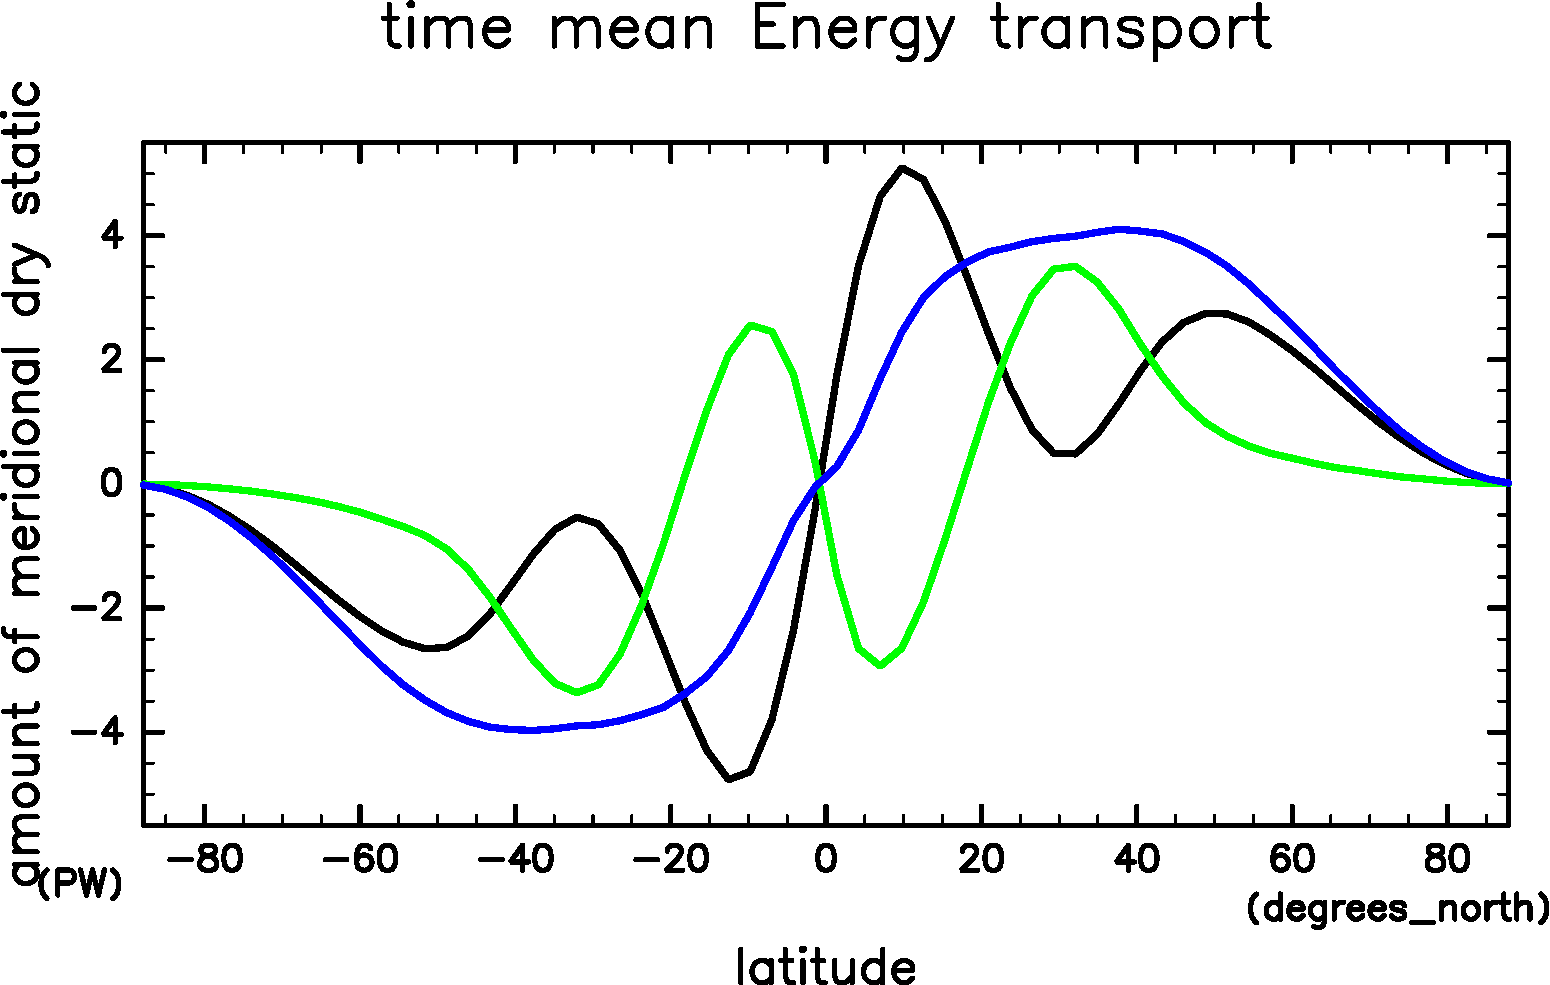
\includegraphics[width=\columnwidth]{S1366/EngyFlx,time=14600:14965-crop-rotate.pdf}
		\caption{\(S=1366\hmu{W/m^2}\)}
	\end{subfigure}
	\begin{subfigure}{.4\textwidth}
		\centering
		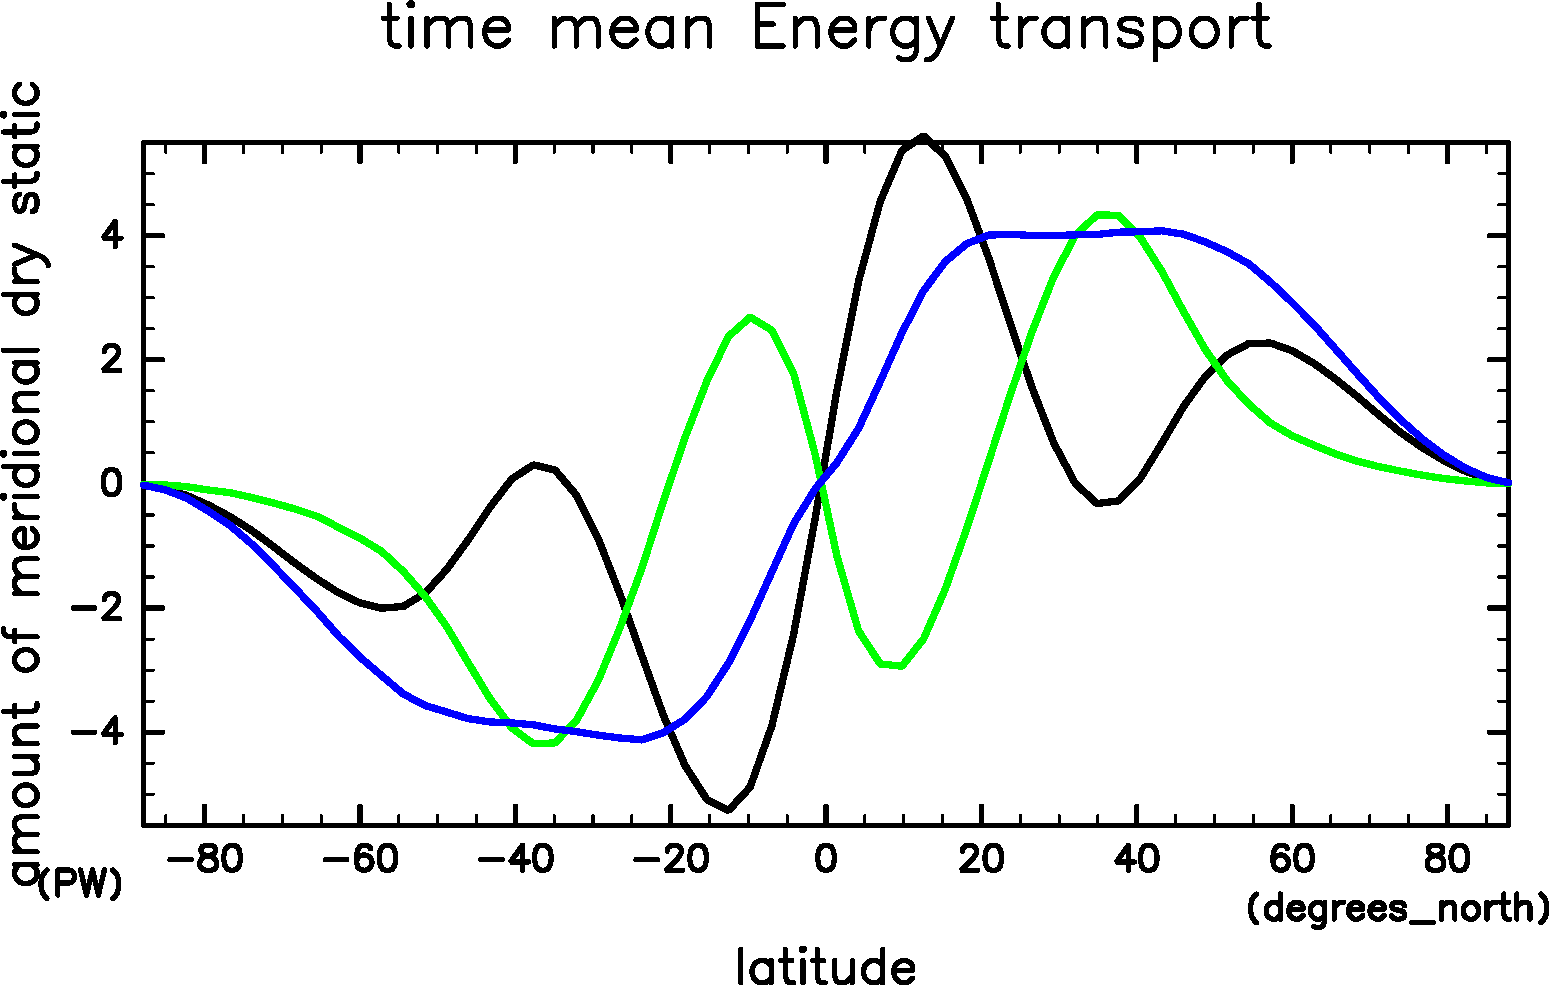
\includegraphics[width=\columnwidth]{S1500/EngyFlx,time=3650:4015-crop-rotate.pdf}
		\caption{\(S=1500\hmu{W/m^2}\)}
	\end{subfigure}
	\begin{subfigure}{.4\textwidth}
		\centering
		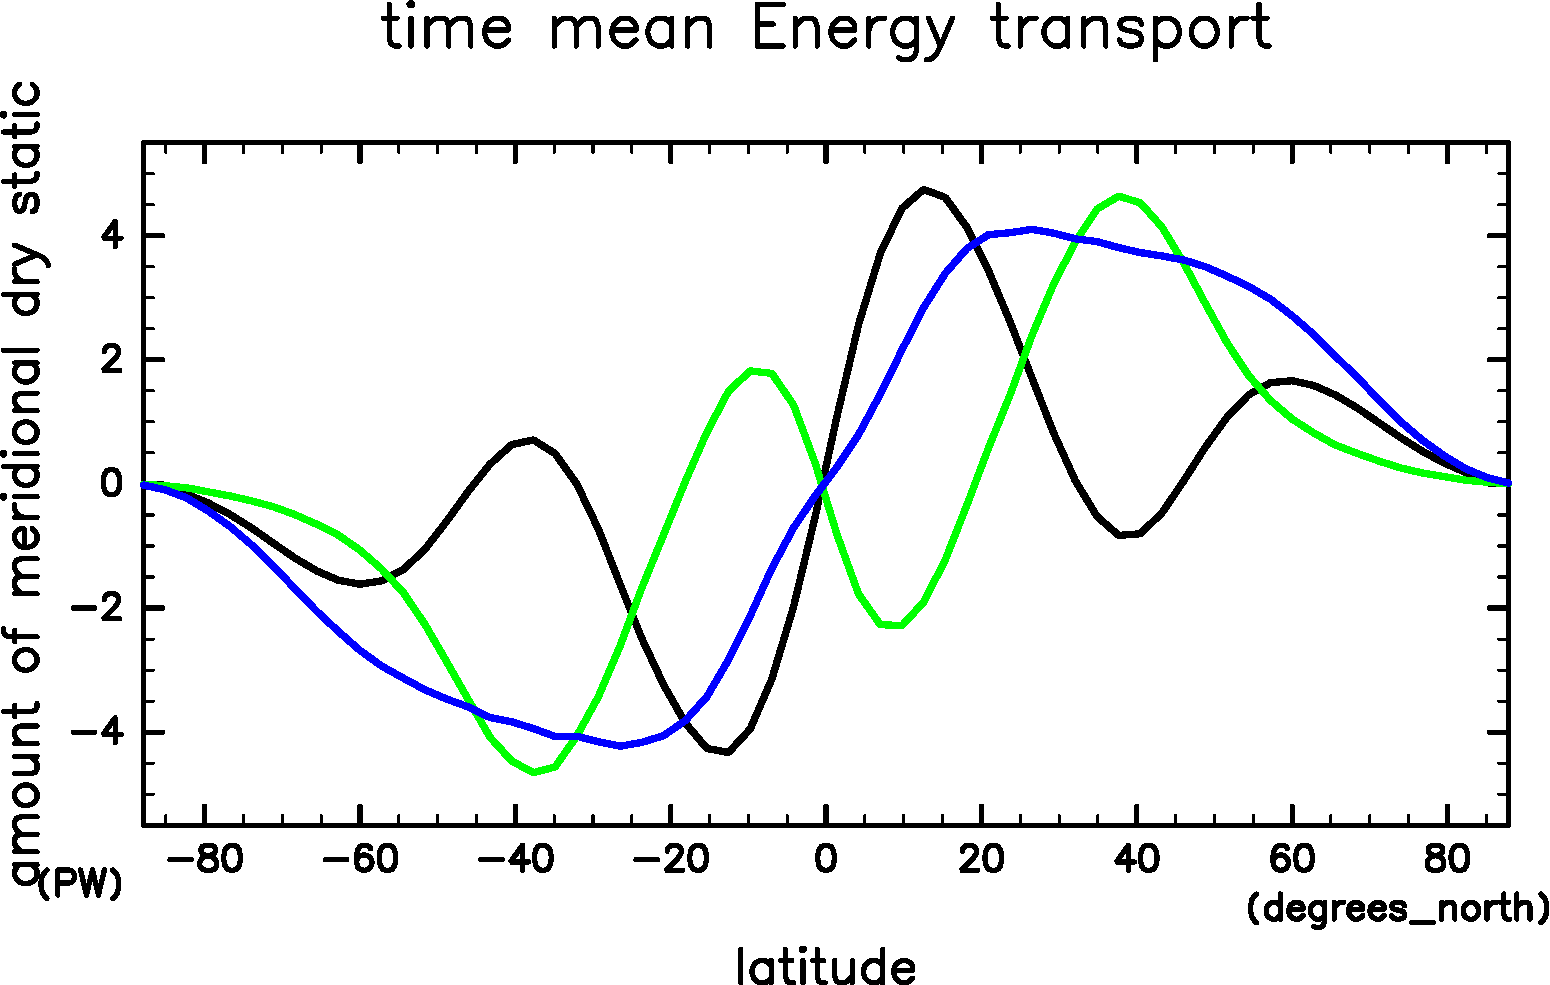
\includegraphics[width=\columnwidth]{S1600/EngyFlx,time=3650:4015-crop-rotate.pdf}
		\caption{\(S=1600\hmu{W/m^2}\)}
	\end{subfigure}
	\begin{subfigure}{.4\textwidth}
		\centering
		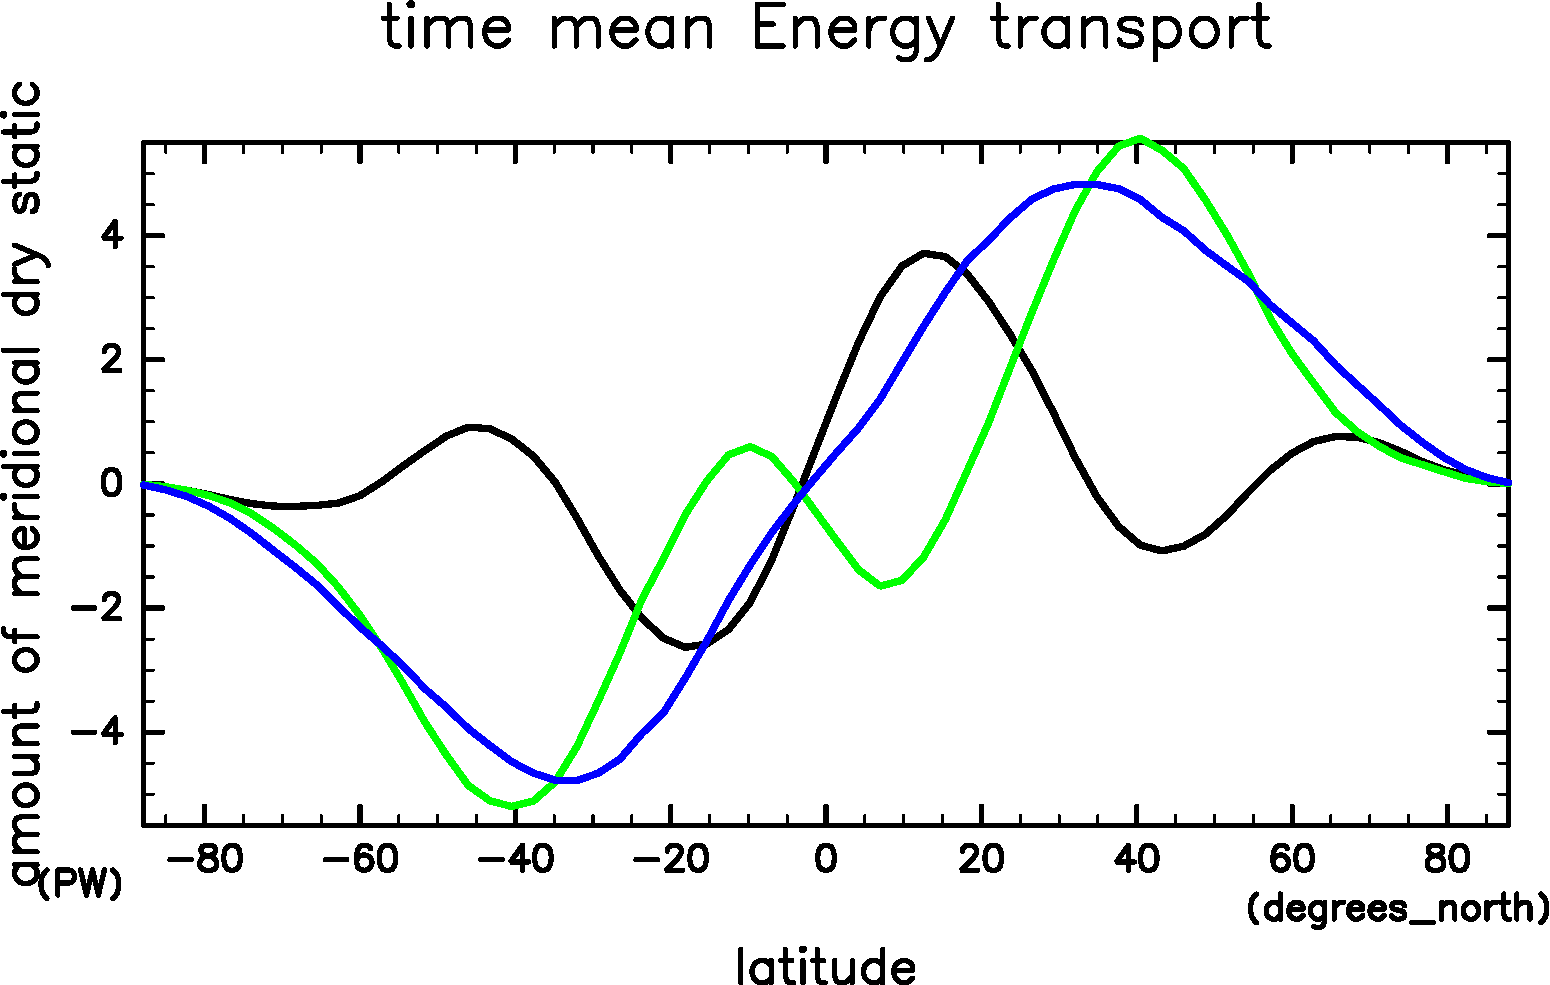
\includegraphics[width=\columnwidth]{S1800/EngyFlx,time=3650:4015-crop-rotate.pdf}
		\caption{\(S=1800\hmu{W/m^2}\)}
	\end{subfigure}
	\begin{subfigure}{.4\textwidth}
		\centering
		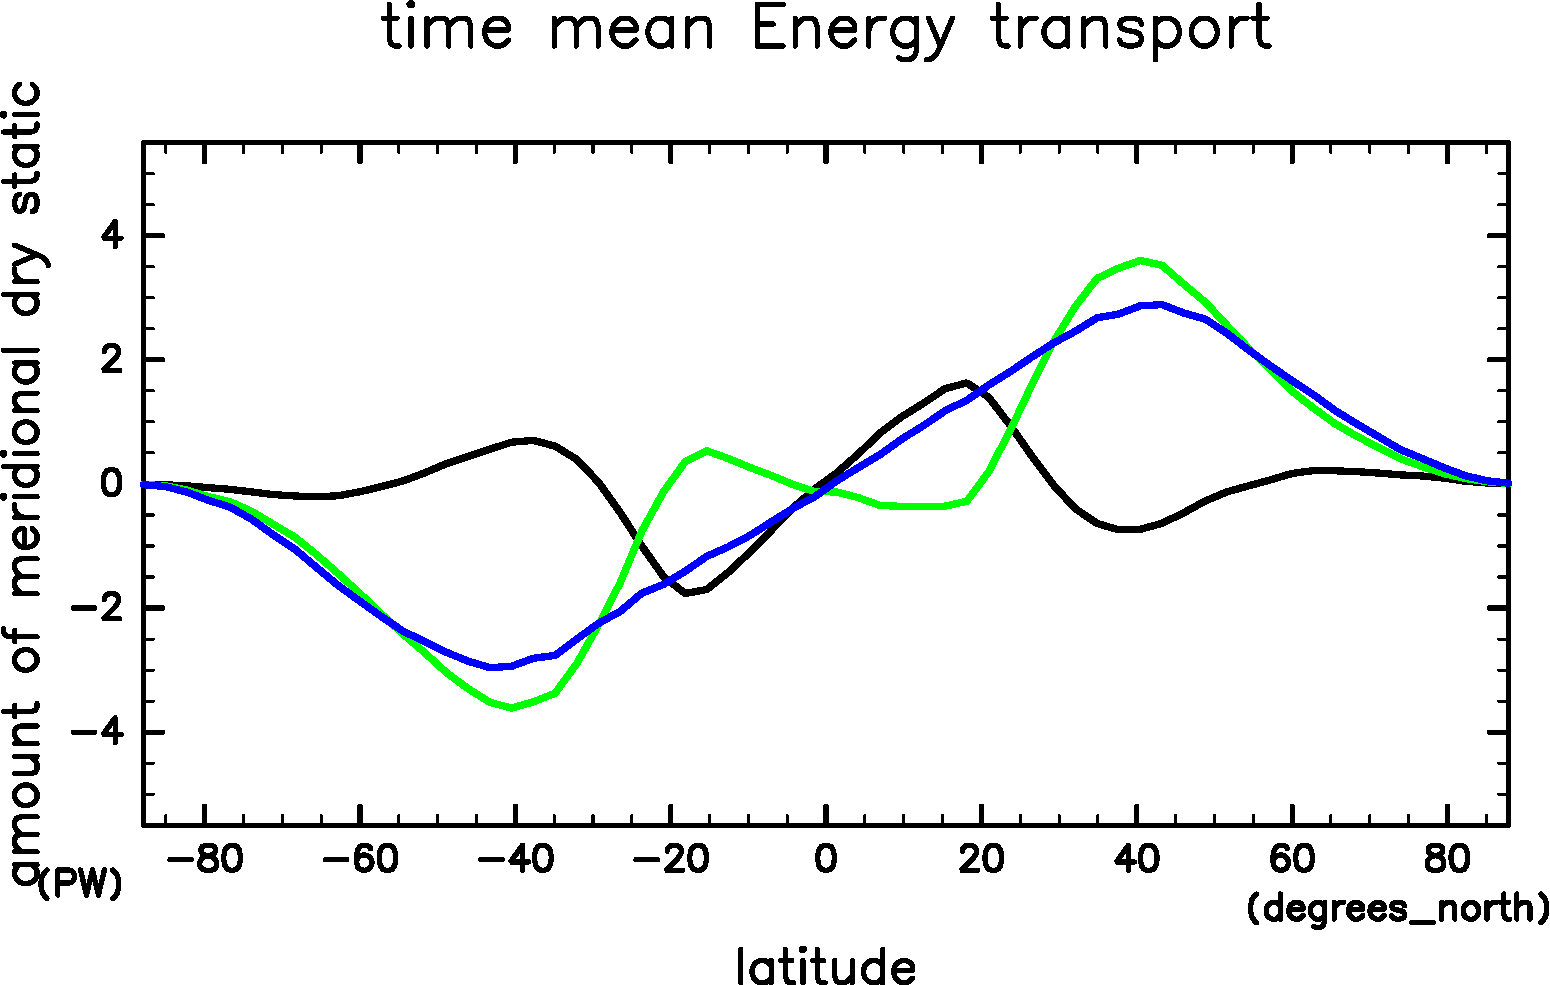
\includegraphics[width=\columnwidth]{S2000/EngyFlx,time=7300:7665-crop-rotate.pdf}
		\caption{\(S=2000\hmu{W/m^2}\)}
	\end{subfigure}
	\caption[各実験での時間平均・東西平均された南北熱輸送量]{
		各実験での時間平均・東西平均された南北熱輸送量。
		緑線が潜熱輸送、黒線が乾燥静的エネルギーの輸送、青線が全熱輸送量。
	}\label{EnFlx}
\end{figure}

\begin{figure}[t]
	\centering
	\begin{subfigure}{.4\textwidth}
		\centering
		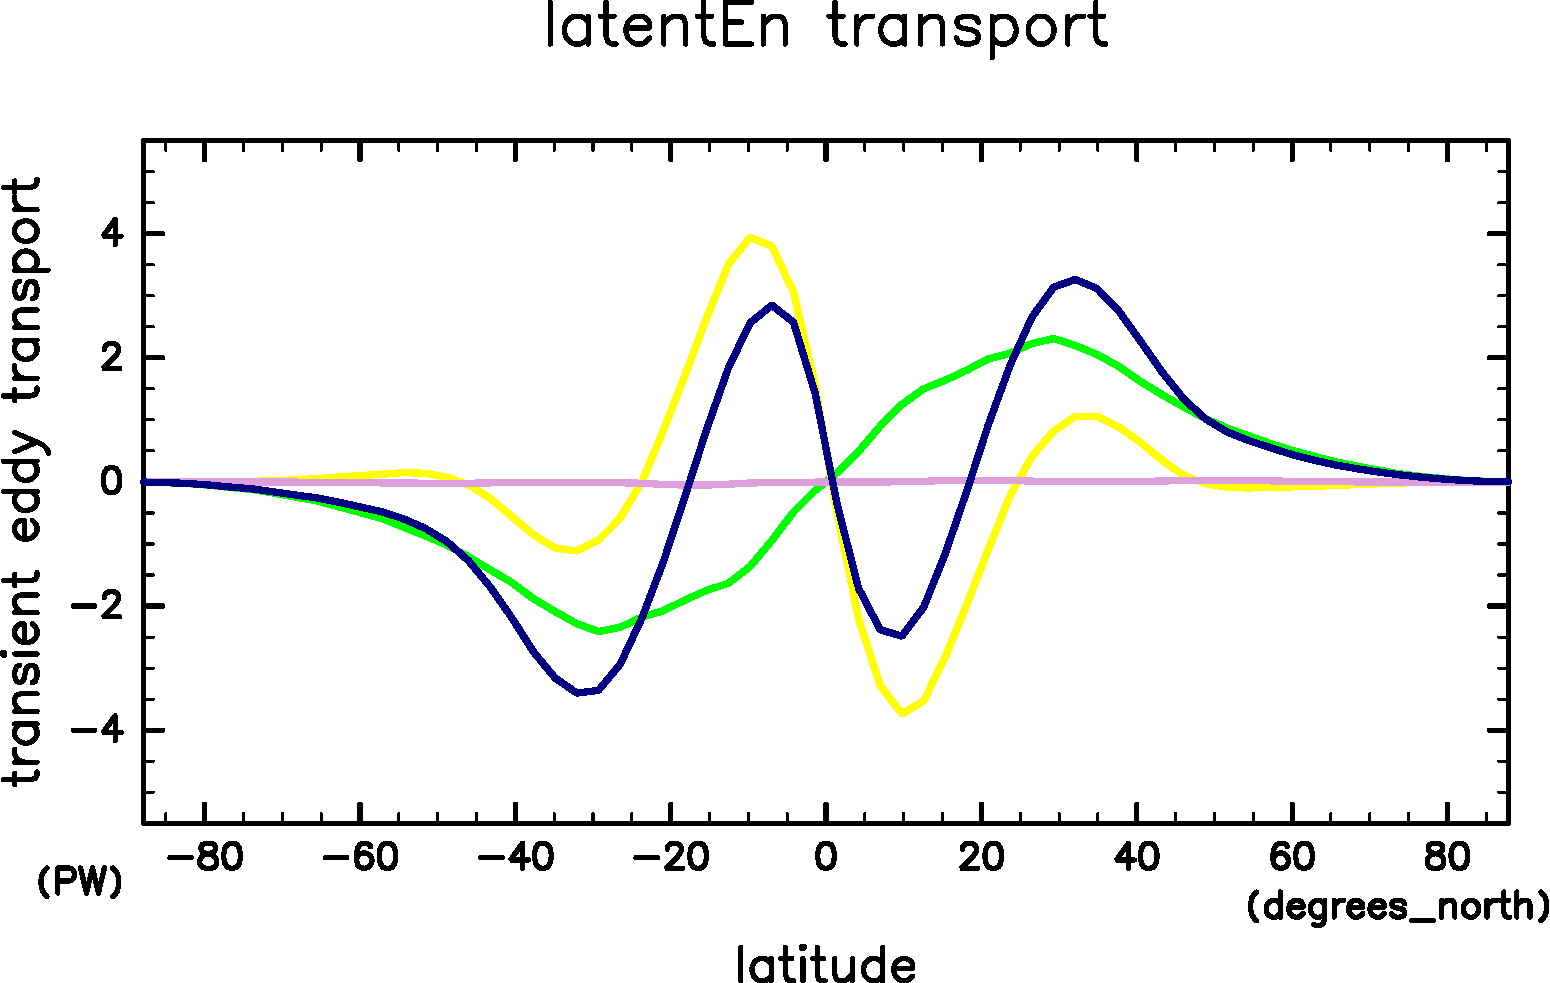
\includegraphics[width=\columnwidth]{S1366/MeriHeatTrans@latentEn,time=14600:14965-crop-rotate.pdf}
		\caption{\(S=1366\hmu{W/m^2}\)}
	\end{subfigure}
	\begin{subfigure}{.4\textwidth}
		\centering
		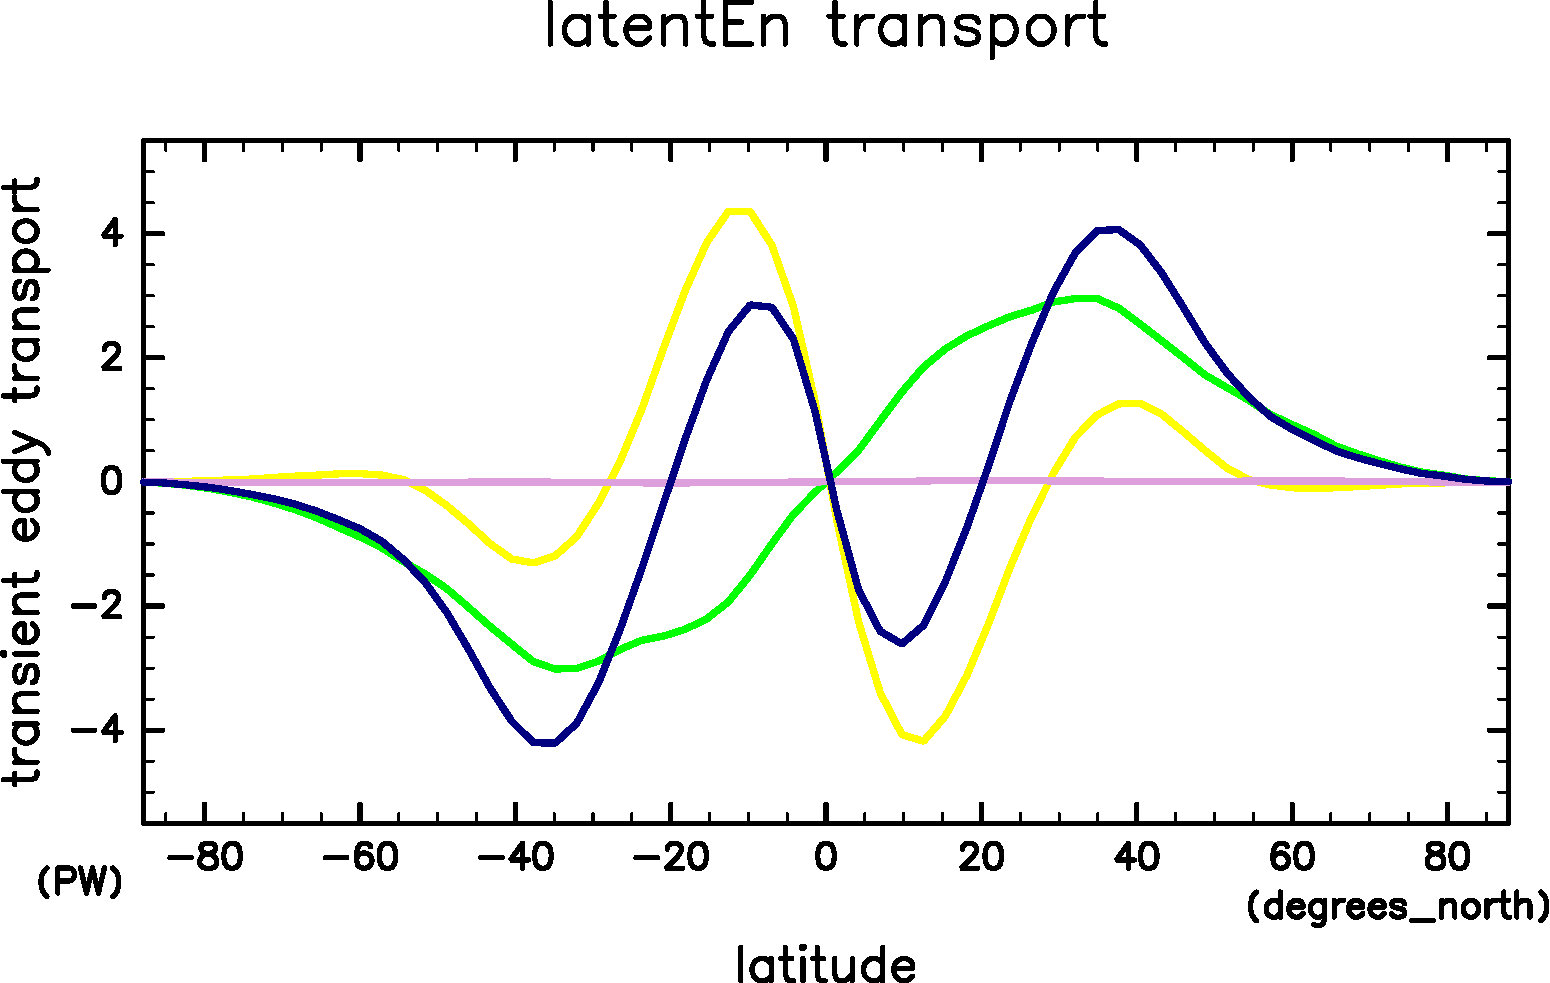
\includegraphics[width=\columnwidth]{S1500/MeriHeatTrans@latentEn,time=3650:4015-crop-rotate.pdf}
		\caption{\(S=1500\hmu{W/m^2}\)}
	\end{subfigure}
	\begin{subfigure}{.4\textwidth}
		\centering
		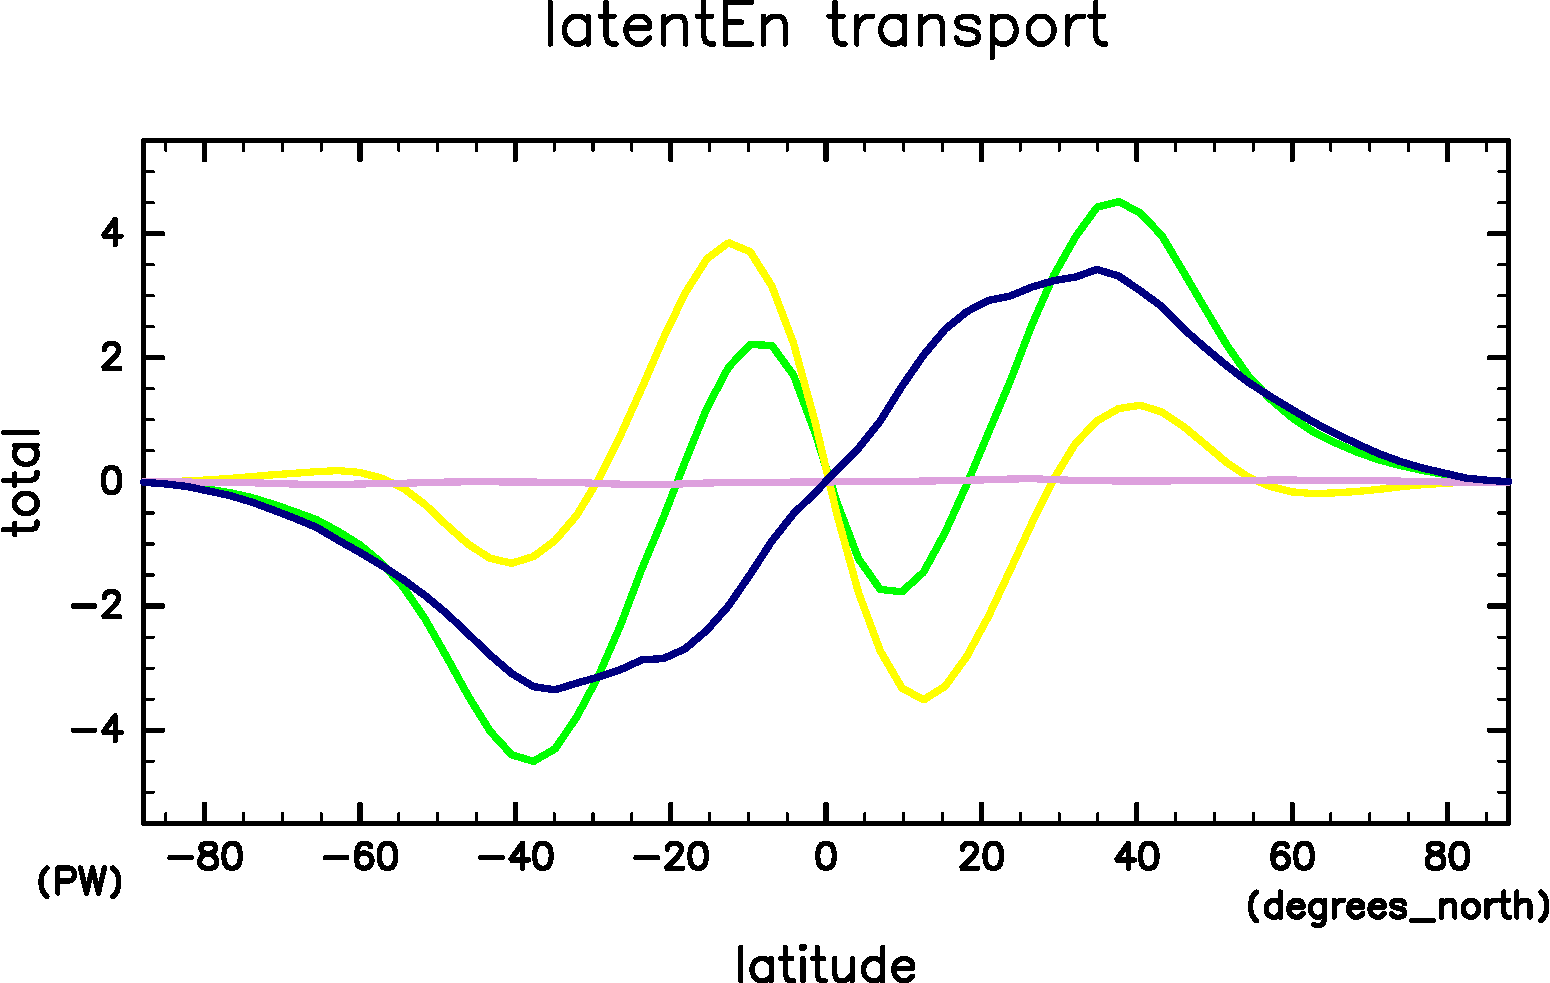
\includegraphics[width=\columnwidth]{S1600/MeriHeatTrans@latentEn,time=3650:4015-crop-rotate.pdf}
		\caption{\(S=1600\hmu{W/m^2}\)}
	\end{subfigure}
	\begin{subfigure}{.4\textwidth}
		\centering
		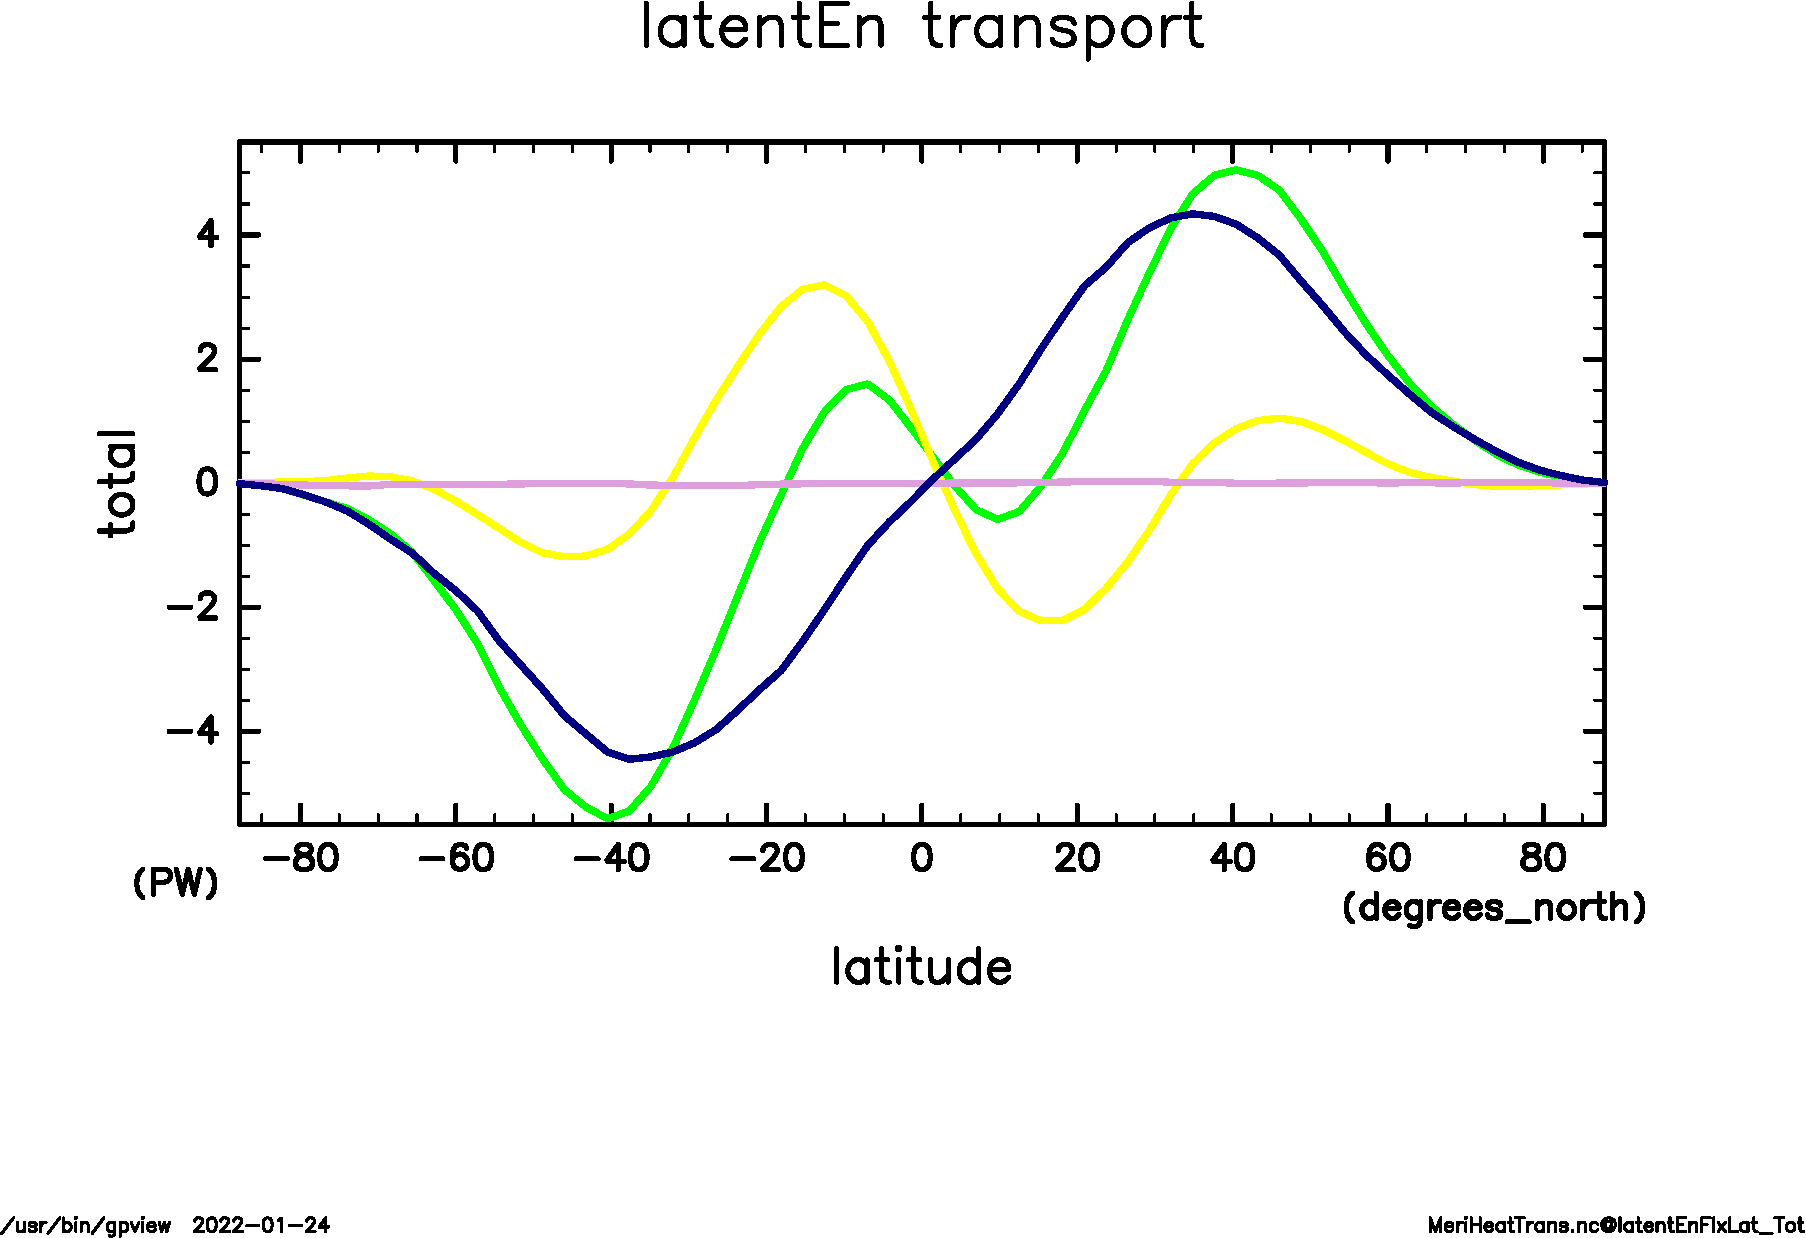
\includegraphics[width=\columnwidth]{S1800/MeriHeatTrans@latentEn,time=3650:4015-crop-rotate.pdf}
		\caption{\(S=1800\hmu{W/m^2}\)}
	\end{subfigure}
	\begin{subfigure}{.4\textwidth}
		\centering
		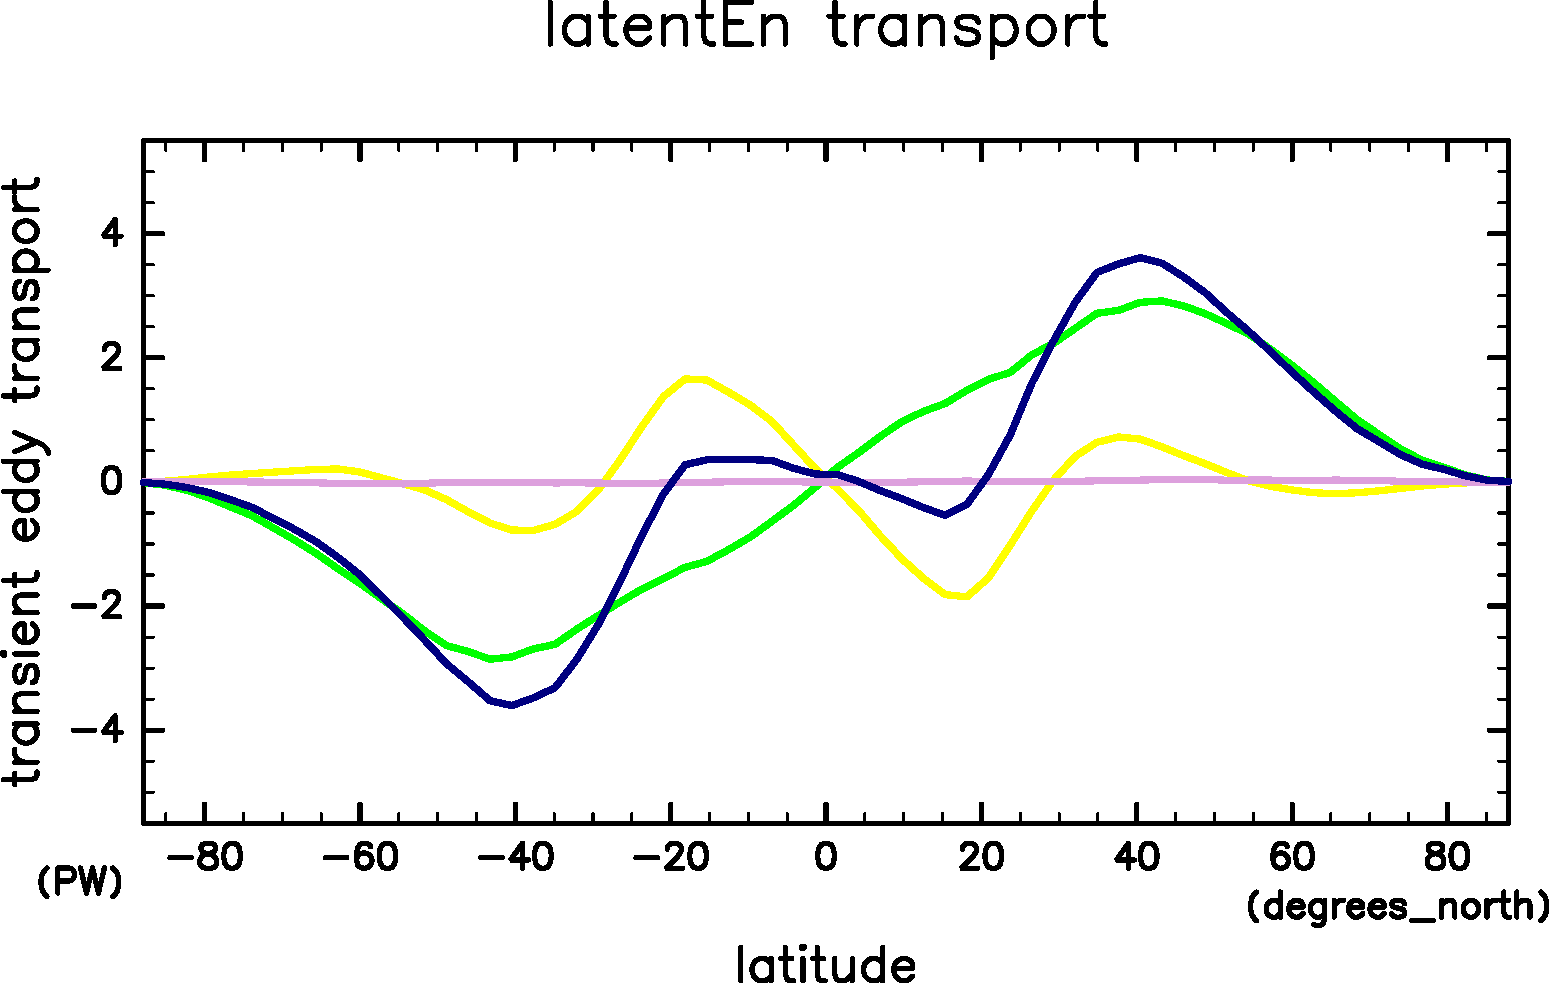
\includegraphics[width=\columnwidth]{S2000/MeriHeatTrans@latentEn,time=7300:7665-crop-rotate.pdf}
		\caption{\(S=2000\hmu{W/m^2}\)}
	\end{subfigure}
	\caption[各実験での潜熱輸送]{
		各実験での潜熱輸送。青線が全輸送量、黄線が平均子午面循環による輸送量、
		桃線が停滞性擾乱による輸送量、緑線が移動性擾乱による輸送量。
	}\label{潜熱}
\end{figure}

\begin{figure}[t]
	\centering
	\begin{subfigure}{.4\textwidth}
		\centering
		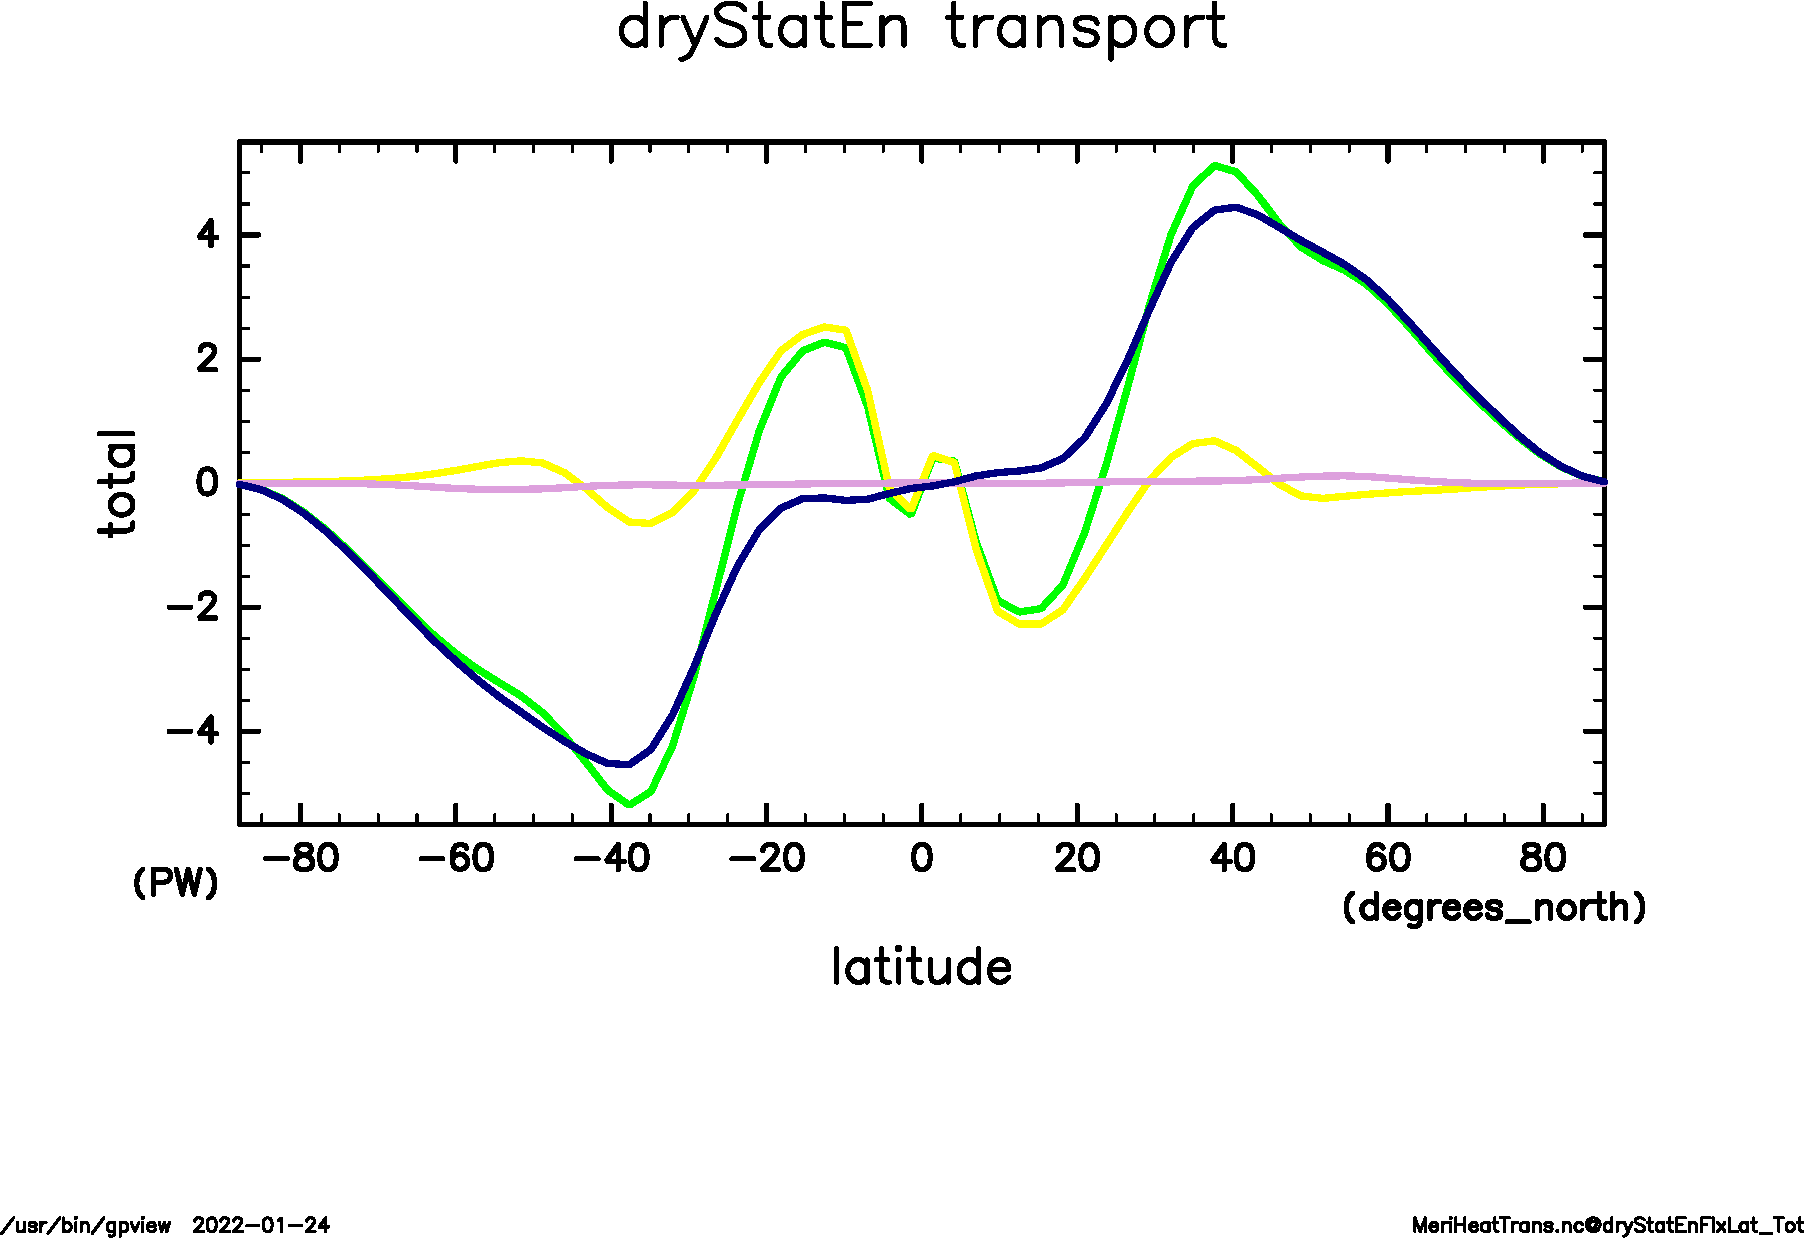
\includegraphics[width=\columnwidth]{S1366/MeriHeatTrans@dryStatEn,time=14600:14965-crop-rotate.pdf}
		\caption{\(S=1366\hmu{W/m^2}\)}
	\end{subfigure}
	\begin{subfigure}{.4\textwidth}
		\centering
		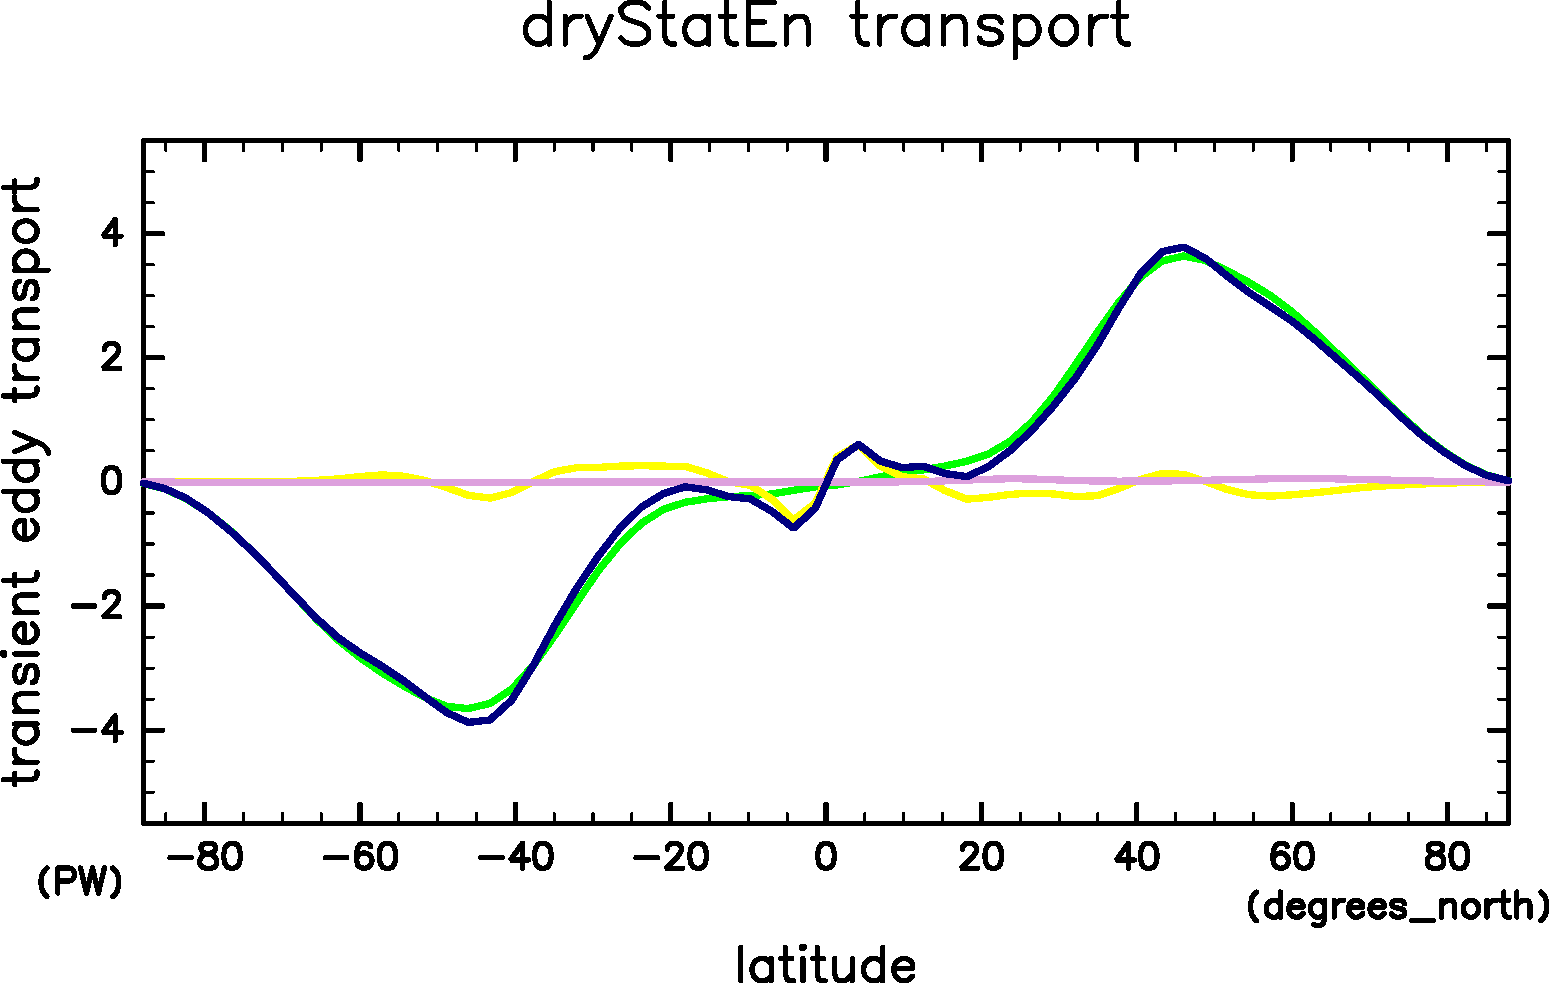
\includegraphics[width=\columnwidth]{S1500/MeriHeatTrans@dryStatEn,time=3650:4015-crop-rotate.pdf}
		\caption{\(S=1500\hmu{W/m^2}\)}
	\end{subfigure}
	\begin{subfigure}{.4\textwidth}
		\centering
		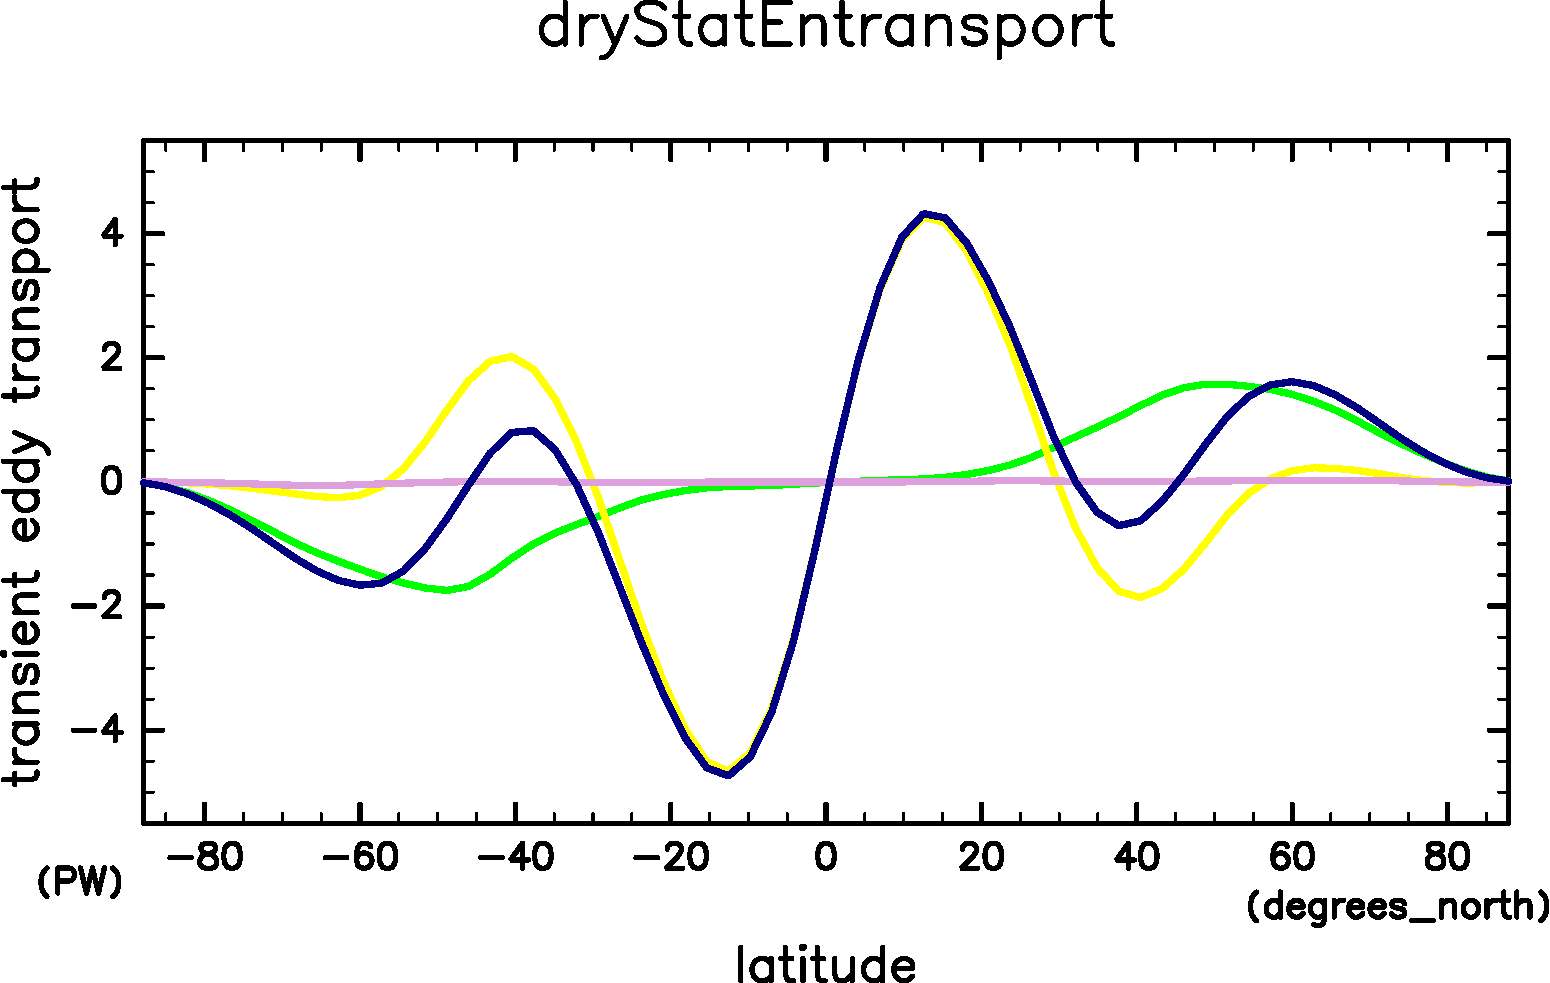
\includegraphics[width=\columnwidth]{S1600/MeriHeatTrans@dryStatEn,time=3650:4015-crop-rotate.pdf}
		\caption{\(S=1600\hmu{W/m^2}\)}
	\end{subfigure}
	\begin{subfigure}{.4\textwidth}
		\centering
		\includegraphics[width=\columnwidth]{S1800/MeriHeatTrans@dryStatEn,time=3650:4015-crop-rotate.pdf}
		\caption{\(S=1800\hmu{W/m^2}\)}
	\end{subfigure}
	\begin{subfigure}{.4\textwidth}
		\centering
		\includegraphics[width=\columnwidth]{S2000/MeriHeatTrans@dryStatEn,time=7300:7665-crop-rotate.pdf}
		\caption{\(S=2000\hmu{W/m^2}\)}
	\end{subfigure}
	\caption[各実験での乾燥静的エネルギー輸送]{
		各実験での乾燥静的エネルギー輸送。青線が全輸送量、黄線が平均子午面循環による輸送量、
		桃線が停滞性擾乱による輸送量、緑線が移動性擾乱による輸送量。
	}\label{乾燥静的エネルギー}
\end{figure}


図 \ref{EnFlx} を詳しく見ると、潜熱輸送は低緯度と高緯度にピークを持っており、
乾燥静的エネルギー輸送は中緯度にピークを持っている。
潜熱輸送の低緯度のピークに対応する部分では、大気下層で低緯度向きの平均南北風
が卓越している。そして、比湿は低緯度で大きく、大気下層で大きくなっているので、
低緯度側のピークのほうが大きくなる。

\begin{itemize}
	\item S1800 までは、比湿が大きくなるので潜熱輸送が大きくなる。
	\item 太陽定数が大きくなると、上空の南北風が小さくなるので \(gzv\) が小さくなり、
		乾燥静的エネルギーの輸送が小さくなる。
	\item S2000 は南北風が小さいので南北熱輸送が少ない。
	\item 地形がないので停滞性擾乱による輸送は小さい。
	\item 移動性擾乱による潜熱輸送は、どの太陽定数でも中緯度で大きくなり、
		中緯度での潜熱輸送の大部分を占める。
	\item 乾燥静的エネルギーの輸送は、低緯度では平均子午面循環によるものが大きく、
		中緯度・高緯度では移動性擾乱によるものが大きい。
\end{itemize}

\begin{itemize}
	\item 
\end{itemize}

\end{document}
